\documentclass[sigchi]{acmart}

\usepackage{booktabs} % For formal tables
\usepackage[normalem]{ulem} % strikethrough
% \usepackage{cancel}% strikethrough
\usepackage{soul}% strikethrough

\newcommand{\rev}[1]{\textcolor{black}{#1}}
\newcommand{\toolname}{DataToon}
\newcommand{\bstart}[1]{\vspace{1mm} 
\noindent{\textbf{#1}}}
\newcommand{\bcstart}[1]{\vspace{1mm} \noindent{\textbf{#1:}}}
\newcommand{\bpstart}[1]{\vspace{1mm} \noindent{\textbf{#1.}}}
\long\def\ignore#1{}

% show TODO and author comments:
\definecolor{nam}{RGB}{31,119,180}
\definecolor{matt}{RGB}{255,127,14}
\definecolor{benjamin}{RGB}{44,160,44}
\definecolor{nathalie}{RGB}{214,39,40}
\definecolor{haijun}{RGB}{148,103,189}
\definecolor{michael}{RGB}{140,86,75}
\definecolor{ken}{RGB}{27,119,194}
\definecolor{michel}{RGB}{23,190,207}
\definecolor{hanspeter}{RGB}{188,189,34}

\definecolor{add}{HTML}{009688}
\definecolor{delete}{HTML}{F44336}



\newcommand{\cf}{cf.}
\newcommand{\etal}{et al.}
\newcommand{\eg}{e.g.,}
\newcommand{\ie}{i.e.,}
\newcommand{\todo}[1]{\textbf{\textcolor{magenta}{#1}}}
\newcommand{\added}[1]{\textcolor{add}{#1}}
\newcommand{\deleted}[1]{\textcolor{delete}{\sout{#1}}}

\newcommand{\white}[1]{\textcolor{white}{#1}}

\newcommand{\nam}[1]{\textbf{\textcolor{nam}{\{NWK: #1\}}}}
\newcommand{\matt}[1]{\textcolor{matt}{\textbf{\{MB: #1\}}}}
\newcommand{\ben}[1]{\textcolor{benjamin}{\textbf{\{BB: #1\}}}}
\newcommand{\nat}[1]{\textcolor{nathalie}{\textbf{\{NHR: #1\}}}}
\newcommand{\haijun}[1]{\textbf{\textcolor{haijun}{\{HX: #1\}}}}
\newcommand{\michael}[1]{\textcolor{michael}{\textbf{\{MM: #1\}}}}
\newcommand{\ken}[1]{\textcolor{ken}{\textbf{\{KH: #1\}}}}
\newcommand{\michel}[1]{\textcolor{michel}{\textbf{\{MP: #1\}}}}
\newcommand{\hanspeter}[1]{\textcolor{hanspeter}{\textbf{\{HP: #1\}}}}

% \newcommand{\matt}[1]{}

% Copyright
% \setcopyright{none}
% \setcopyright{acmcopyright}
\setcopyright{acmlicensed}
%\setcopyright{rightsretained}
%\setcopyright{usgov}
%\setcopyright{usgovmixed}
%\setcopyright{cagov}
% \setcopyright{licensedcagov}
%\setcopyright{cagovmixed}
%\setcopyright{licensedothergov}


\copyrightyear{2019} 
\acmYear{2019} 
% \setcopyright{acmlicensed}
\acmConference[CHI 2019]{CHI Conference on Human Factors in Computing Systems Proceedings}{May 4--9, 2019}{Glasgow, Scotland UK}
\acmBooktitle{CHI Conference on Human Factors in Computing Systems Proceedings (CHI 2019), May 4--9, 2019, Glasgow, Scotland UK}
\acmPrice{15.00}
\acmDOI{10.1145/3290605.3300335}
\acmISBN{978-1-4503-5970-2/19/05}

% Authors, replace the red X's with your assigned DOI string during the rightsreview eform process.

\settopmatter{printacmref=true}
\fancyhead{}


\begin{document}
\title[\toolname{}]{\toolname{}: Drawing Data Comics About Dynamic Networks with Pen + Touch Interaction}
% \titlenote{Produces the permission block, and
%   copyright information}
% \subtitle{Extended Abstract}
% \subtitlenote{The full version of the author's guide is available as
%   \texttt{acmart.pdf} document}

\author{
Nam Wook Kim\textsuperscript{1,2} \space\space\space
Nathalie Henry Riche\textsuperscript{2} \space\space\space
Benjamin Bach\textsuperscript{3} \space\space\space
Guanpeng Xu\textsuperscript{4} \space\space\space
Matthew Brehmer\textsuperscript{2} \\
Ken Hinckley\textsuperscript{2} \space\space\space
Michel Pahud\textsuperscript{2} \space\space\space
Haijun Xia\textsuperscript{5} \space\space\space
Michael J. McGuffin\textsuperscript{6} \space\space\space
Hanspeter Pfister\textsuperscript{1}
}


\affiliation{
\textsuperscript{1} Harvard University \space\space\space
\textsuperscript{2} Microsoft Research \\
\textsuperscript{3} University of Edinburgh \space\space\space 
\textsuperscript{4} Philips Academy \space\space\space
\textsuperscript{5} University of Toronto \space\space\space
\textsuperscript{6} \'Ecole de technologie sup\'erieure \\
\{namwkim, pfister\}@g.harvard.edu \space\space\space 
\{nath, mabrehme, kenh, mpahud\}@microsoft.com \\
bbach@inf.ed.ac.uk \space\space\space
gxu19@andover.edu \space\space\space
haijunxiadgp.toronto.edu \space\space\space
michael.mcguffin@etsmtl.ca
}

% \author{Nam Wook Kim}
% \affiliation{Harvard University}
% \email{namwkim@seas.harvard.edu}

% \author{Nathalie Henry Riche}
% \affiliation{Microsoft Research}
% \email{Nathalie.Henry@microsoft.com}

% \author{Benjamin Bach}
% \affiliation{University of Edinburgh}
% \email{bbach@inf.ed.ac.uk}

% \author{Guanpeng Xu}
% \affiliation{Philips Academy}
% \email{giftedbee@gmail.com}

% \author{Matthew Brehmer}
% \affiliation{Microsoft Research}
% \email{mabrehme@microsoft.com}

% \author{Ken Hinckley}
% \affiliation{Microsoft Research}
% \email{kenh@microsoft.com}

% \author{Michel Pahud}
% \affiliation{Microsoft Research}
% \email{mpahud@microsoft.com}

% \author{Haijun Xia}
% \affiliation{University of Toronto}
% \email{haijunxiadgp.toronto.edu}


% \author{Michael McGuffin}
% \affiliation{École de technologie supérieure}
% \email{michael.mcguffin@etsmtl.ca}

% \author{Hanspeter Pfister}
% \affiliation{Harvard University}
% \email{pfister@g.harvard.edu}




% The default list of authors is too long for headers.
\renewcommand{\shortauthors}{N. Kim et al.}


\begin{abstract}
Comics are an entertaining and familiar medium for presenting compelling stories about data. However, existing visualization authoring tools do not leverage this expressive medium. In this paper, we seek to incorporate elements of comics into the construction of data-driven stories about dynamic networks. We contribute \toolname{}, \rev{a flexible data comic storyboarding tool that blends analysis and presentation with pen and touch interactions.} A storyteller can use \toolname{} to rapidly generate visualization panels, annotate them, and position them within a canvas to produce a visual narrative. \rev{In a user study, participants quickly learned to use \toolname{} for producing data comics}.
 

% \added{\toolname{} bridges the current gap between exploration and storytelling in existing tools by enabling a storyteller to rapidly generate visualization panels, as well as to annotate them and arrange them within a canvas to }

% Comics is an entertaining and familiar storytelling medium. Despite its great potential for understanding and communicating complex data, there are few existing tools that leverage the unique form of comics in constructing data-driven stories.  medium in . 

% In this paper, we investigate ways to incorporate the unique form of comics to construct data-driven stories.


% This paper  presents \toolname{}, a browser-based tool for creating highly expressive data comics about dynamic networks via pen and touch interactions. 

% The need to craft expressive visuals from data, maintain consistency accross panels and compose them in space to create a compelling narrative are unique challenges of data comics that are not well supported by current authoring tools. 

% \toolname{} provides a direct manipulation pen + touch interface along with expressive annotation options, allowing storytellers to sketch with data and experiment with different designs to produce dynamic network comics. 

% \toolname{} smoothly integrates data binding, visual encoding, story authoring, and annotation, activities which would have previously required use of multiple tools with little or no connection to the underlying data. We conducted a qualitative study to evaluate the usability and demonstrate the expressiveness of our tool through examples.
\end{abstract}


\begin{CCSXML}
<ccs2012>
<concept>
<concept_id>10003120.10003145.10003151</concept_id>
<concept_desc>Human-centered computing~Visualization systems and tools</concept_desc>
<concept_significance>300</concept_significance>
</concept>
</ccs2012>
\end{CCSXML}

\ccsdesc[300]{Human-centered computing~Visualization systems and tools}

\keywords{Data comics, pen + touch interfaces, direct manipulation, storytelling, dynamic networks, data visualization.}

\begin{teaserfigure}
  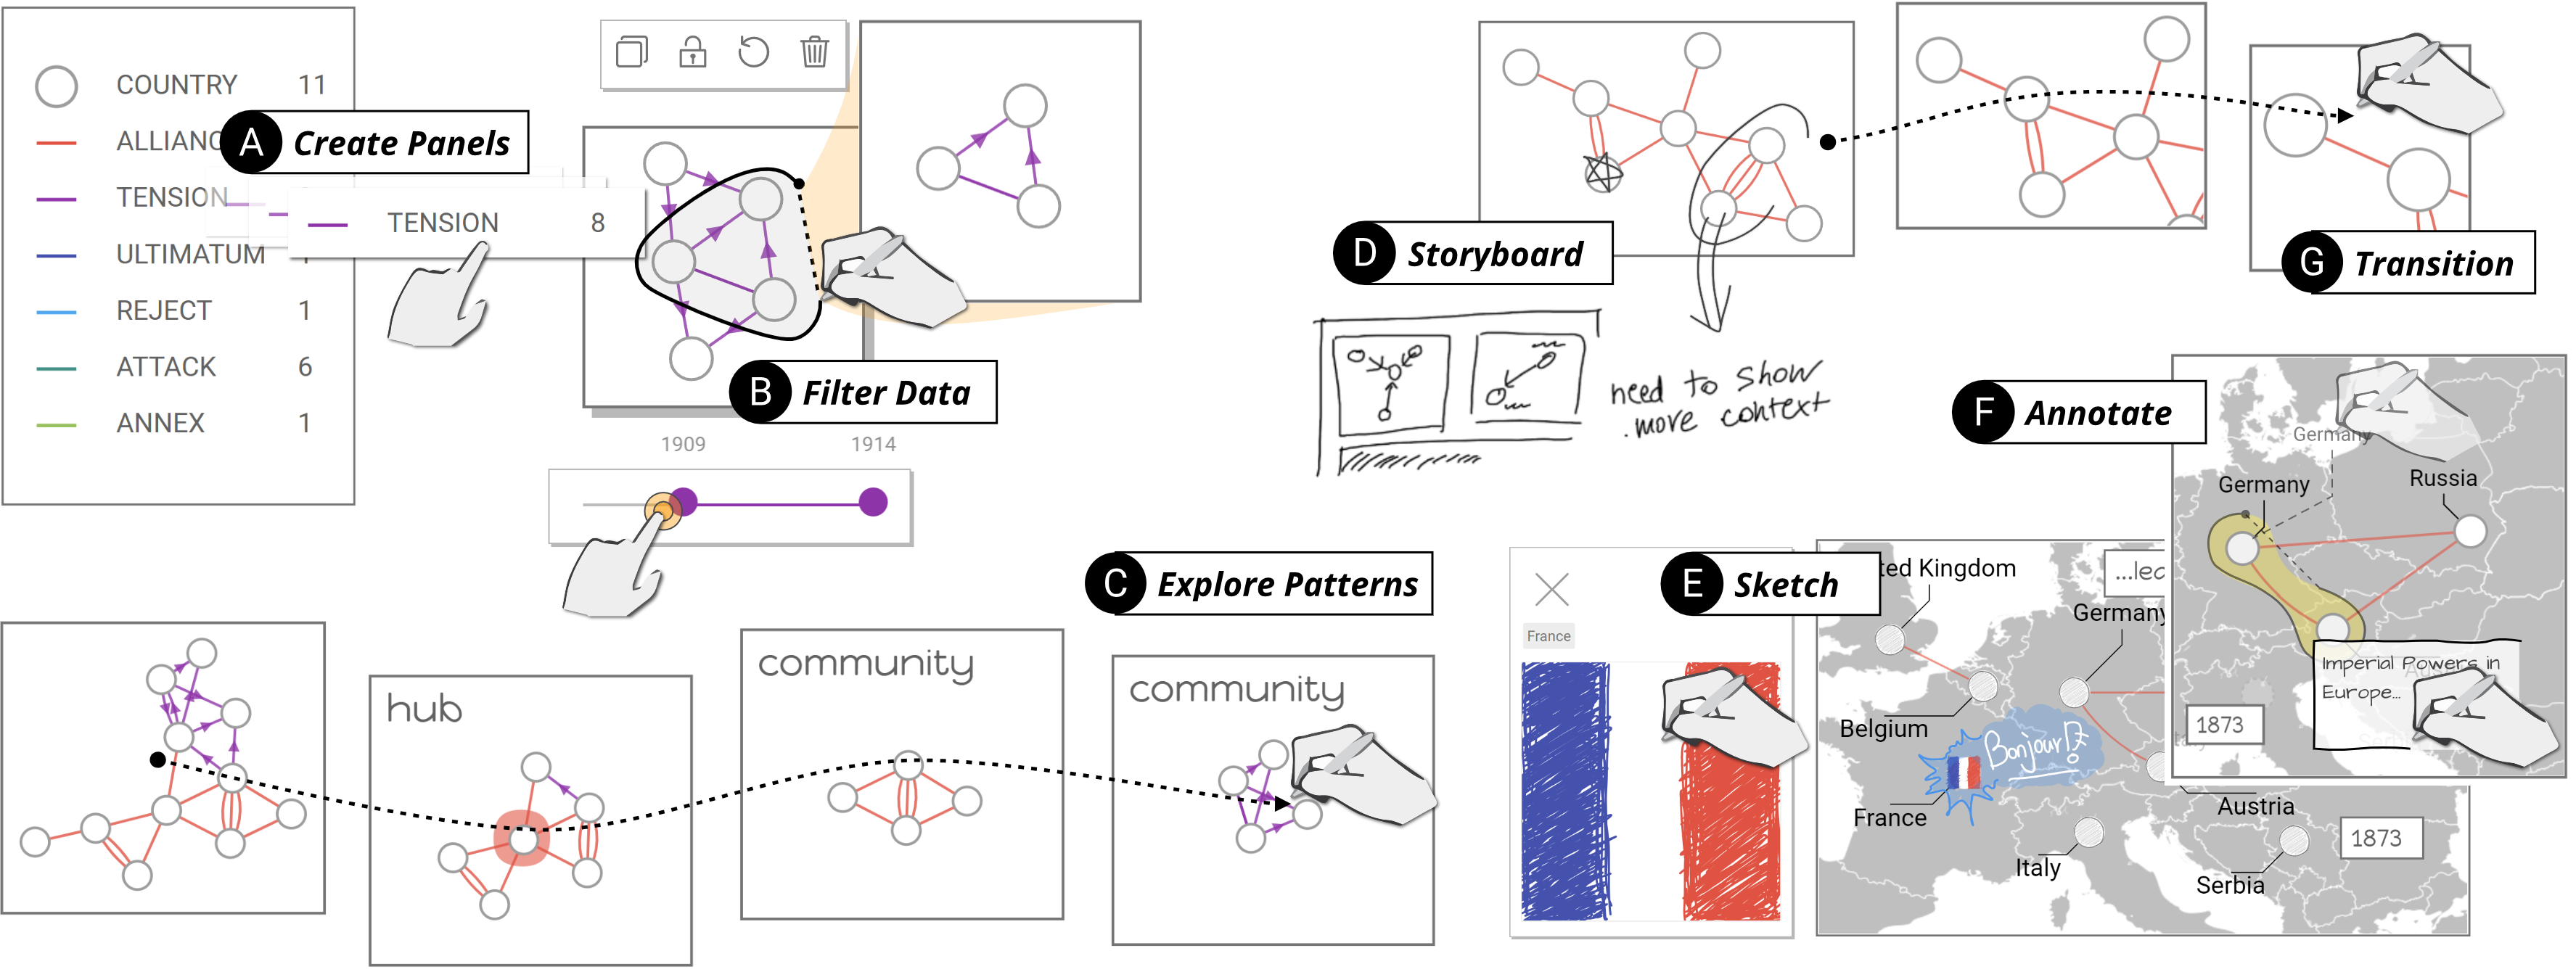
\includegraphics[width=1.0\textwidth]{figures/teaser.png}
  \caption{\toolname{} is a pen \& touch environment for producing data comics. A storyteller can rapidly isolate aspects of their data via filtering and pattern detection, as well as assemble a rich narrative via annotation and automatic panel transitions.}
  \centering
  \label{fig:teaser}
\end{teaserfigure} 

\maketitle
\renewcommand{\shortauthors}{Nam et al.}
% \input{paper-body}

\section{Introduction}
% \nat{Try to make intro fit in one page with teaser}

Visualization is a pivotal component in data-driven storytelling, providing an audience with the means to understand patterns in data without requiring advanced statistical literacy~\cite{ddsbook}. One genre of data-driven storytelling~\cite{segel2010narrative} is the {\it data comic}~\cite{bach2017emerging}, in which a narrative grounded in data is conveyed by leveraging the well-established visual language of comics~\cite{mccloud1993understanding}. Data comics integrate captions and annotations with visualization, suppressing the complexity of data by incrementally revealing aspects of the data across multiple panels, arranged thoughtfully on one or more pages~\cite{bachdesign,wang2019study}. 

A recently curated collection of manually-created data comics~\cite{datacomicsnet} demonstrates the richness of this genre and its applicability to telling stories about datasets of different natures.
%\matt{We need to answer the of {\it why dynamic networks?} up front}
From a storytelling standpoint, one of the most challenging forms of data is a dynamic network. Dynamic networks appear in many contexts, from analyzing social networks to modeling neural connections in the brain. In addition to evolving in time, such networks may contain multiple types of nodes and links exhibiting different connectivity patterns. Due to this complexity, it is notoriously difficult to communicate insights about dynamic networks to a general audience with a single large visual representation. Since conventional comics often illustrate the dynamic nature of characters and the interactions that occur between them over time by identifying and sequencing salient moments, dynamic networks are ideally suited for a comic treatment~\cite{bach2016telling}. 


However, producing a data comic is a difficult and laborious process, one that involves switching between visualization and graphic design tools~\cite{bigelow2017iterating}, the former being ideal for generating accurate data representations, and the latter being ideal for stylizing visual elements and arrange panels in space. 
While several recent tools support the construction of visual data stories~\cite{kim2017data,satyanarayan2014lyra,xia2018dataink,ren2014ivisdesigner}, they do not take advantage of the comic form as a storytelling medium. Thus authors have to resort to illustration and design tools such as Adobe Illustrator and Photoshop.

%Instead, many tools address the creation of a single visualization, illustrating an individual message as opposed to conveying a holistic narrative~\cite{kim2017data,satyanarayan2014lyra,xia2018dataink,ren2014ivisdesigner}. While other tools offer support for sequencing multiple visualizations to produce a narrative structure, they are limited to a linear slideshow or scrolling format and thus do not support the spatial arrangements that are central to the design of comics~\cite{storypoints,amini2017authoring,conlen2018,gratzl2016visual,mckenna2017visual}. Moreover, existing tools focus on realizing a preconceived story rather than on the process of identifying and refining a narrative, and thus they enforce a rigid workflow in which data exploration is disjoint from designing the audience's experience. This separation hinders rapid experimentation with story ideas, an issue that we address with \toolname{}.


We contribute \toolname{} as a storytelling tool for producing data comics \rev{with a focus on dynamic networks.
\toolname{} offers fluid storyboarding by blending analysis and presentation in a unified environment supported by pen and touch interactions. A storyteller can use \toolname{} to rapidly explore their data and generate visualization panels via interactive filtering and from recommendations of interesting data patterns, resulting in a visual story with custom annotations, automatic panel transitions, and layout templates.}

\rev{The direct manipulation of panels and their data contents further facilitates the storytelling process. Natural touch interaction supports the iteration of story ideas by experimenting with different ways to compose panels and lay them out on a page. The use of a digital pen also allows storytellers to annotate panels with drawings and handwriting, or to draw custom glyphs for data entities. \toolname{} leverages the underlying data to eliminate the tedious duplication of actions necessary in conventional illustration software, such as propagating visual designs to other panels.}


\rev{To demonstrate the expressivity of \toolname{}, we created a set of comics showing different rendering styles, panel layouts, visualization types, and narrative structures.} Results from a reproduction study suggest that novice participants can successfully learn to use \toolname{} with minimal guidance to produce comics about dynamic networks. \rev{Insights about usability that led to improvements of \toolname{} included difficulties in discovering features, the inconsistency of interactions, and the complexity of visualization contents.}

%Storytellers can use \toolname{} to rapidly explore data and generate visualization panels through interactive filtering and recommendations of interesting data patterns. They can author a visually compelling story through custom annotations, automatic panel transitions, and layout templates. Direct manipulation of panels and their data contents with pen and touch interactions facilitates the authoring process. 

%\matt{We need to answer the of {\it why pen + touch?} up front}
%Another distinguishing aspect of many comics is the unique style of the individual illustrators who draw them. 
%We attempt to retain this aspect of comics by leveraging pen-based interactions in \toolname{}, allowing storytellers to stylize nodes and annotate panels to reflect their own custom visual style.
%Beyond styling, \toolname{} features a palette of pen and touch interactions that allow storytellers to directly manipulate panels and their contents.

%With \toolname{}, a storyteller can quickly generate visualization panels to iterate through story ideas by experimenting with different ways to compose panels and lay them out in space. 
%It also provides scaffolding for narrative structures by integrating suggestions, automatic generation of transition panels, and a set of common comic page layouts. 
%Ultimately, the environment is designed to support a flexible workflow integrating data exploration, story authoring, and presentation within in a single tool. 


% A user study with novice users with  designers and data analysts demonstrate its usability (Section 6).
 
%, relying on data binding to ensure visual consistency between the panels
% . To better convey the semantics of the data, 

% We opted to target DataToon to the creation of comics from dynamic multivariate networks. This scope allowed us to build upon previous work~\cite{bach2016telling} which demonstrated the power of the genre for this type of data. 



% \nat{why: creating these things is hard}

% While several recently proposed tools from the research community have aspired to unify this process for infographics~\cite{kim2017data,bigelow2017iterating,liu2018data,Wang2018}, data comics pose unique design challenges. 
% In a data comic, we visualize aspects of the data across multiple panels, and thus the design challenges we face include a need to maintain visual consistency between them~\cite{qu2018keeping} and to provide appropriate transitions from one panel to the next in an effort to convey a coherent narrative. %Another challenge is to remain true to the genre, in the sense that comics are traditionally drawn by hand, allowing each comic artist to develop their own authentic style. 
% They also require crafting expressive visual designs that align well with the semantics of the data and experimenting with different ways to break down the story into panels and arrange them in space. Addressing these challenges with existing tools is extremely tedious and time-consuming.

%One explanation for this lack of examples might be the effort involved in creating compelling comics that  include real-world data and exhibit an appealing visual style. While high-level design patterns for designing data comics have been proposed~\cite{bachdesign}, technically implementing data comics is mostly manual labor, typically involving two distinct families of tools: visualization authoring environments and a graphic design applications. While visualization tools mostly lacks flexible support for adding annotations and customizing graphical elements, graph environments often lack data-driven abstractions and require time-consuming and error-prone manual encoding~\cite{bigelow2014reflections,satyanarayan2014lyra}. 
% Thus, designing the new generation of authoring tools for data-driven storytelling and bridging the gap between two ends of the spectrum, has been an active research area in recent years. 
%While several recently proposed tools from the research community have aspired to unify this process for infographic design~\cite{kim2017data,bigelow2017iterating,liu2018data,Wang2018}, 
%Moreover, data comics pose unique design challenges such as laying out panels, assure consistency between panels and visualizations.

%and we are unaware of previous work that proposes an authoring approach for this genre. 
%In a data comic, we visualize aspects of the data across multiple panels, and thus the design challenges we face include a need to maintain visual consistency between them~\cite{qu2018keeping} and to provide appropriate transitions from one panel to the next in an effort to convey a coherent narrative. 
%Another challenge is to remain true to the genre, in the sense that comics are traditionally drawn by hand, allowing each comic artist to develop their own authentic style.
%Addressing these challenges with existing tools would be extremely tedious and time-consuming. 

% Composing the spatial layout of panels, styling visual elements while ensuring correct data representation make data comics extremely time-consuming to create even for data visualization and graphic design professionals.

 %Data comics involving multiple panels still requires to iterate between visualization creation tools and graphic design tools. In addition, the specificity of data comics poses further challenges such as managing multiple panels of visualizations (a data story usually has more than one visualization as supporting evidence) and maintaining consistency across them. Altogether, using existing tools to create compelling-looking and attractive examples of data comics requires significant expertise and tool skills. 

% \ben{\textit{start with data comics and talk about necessity and difficulty in creating comics: 
% }Comics are emerging as a story-telling medium for data through their unique combination of narration and visual content, as well as their familiarity and accessibility (web, paper, other offline media, etc.)~\cite{bach2017emerging}. Data comics have been presented for networks~\cite{bach2016telling} and many other domains\footnote{\url{http://datacomics.net}}. While generally being perceived as rather 'simple' to create, significant expertise and tool skills (e.g. Photoshop, Illustrator) are required to create compelling-looking and attractive examples of data comics. Moreover, data comics visualize data.
% }

% \nat{what we did} 

% This paper introduces DataToon, an editor for authoring data-driven data comics via direct pen + touch interactions. 
% \matt{explain why dynamic networks}
%We target dynamic and geographic networks as they are a form of data having a complexity that is often best communicated via multiple views. 
%Furthermore, our focus on dynamic networks allows us to realize a speculative design space proposed for depicting this form of data in comic form~\cite{bach2016telling,bach2017emerging,bachdesign}.  
% DataToon enables authors to quickly generate panels from data, relying on data binding to ensure consistency of the visuals. It also provides direct and fluid interactions to explore different expressive visual designs by sketching, and to experiment with different ways to break down panels and lay them out in space by touch interactions. DataToon also features mechanisms to assist in data comic creation, such as the automatic generation of transitions between two panels. We opted to target DataToon to the creation of comics from dynamic multivariate networks. This scope allowed us to build upon previous work~\cite{bach2016telling} which demonstrated the power of the genre for this type of data. 
%rovides data binding data comics and provides features to integrate the data into the design process, e.g., combine exploration and presentation, propagate styles, and automatically create transitions between panels. \ben{are these the most important ones?}.

%In this paper, we describe how the design decisions leading to \toolname{} are rooted in the analysis of the comic form, as well as how we overcame the aforementioned challenges with respect to comic authoring. 
% \matt{the following repeats much of the preceding paragraph}
% The design of our tool is deeply , meaning that the core elements of comics (words, pictures, and panels) are synthesized with the design elements of data stories (visualizations, annotations, and story pieces). 
% \toolname{} offers intuitive, direct manipulation through pen and touch in order to create, manipulate, and customize the elements of data comics. 
% \toolname{} smoothly integrates visual encoding, story authoring, and annotation, activities which would have previously required use of multiple tools with little or no connection to the underlying data. 
% This enables flexible and iterative design and ensures the visual consistency~\cite{qu2018keeping} across multiple panels. 
% We start with a reflection on design challenges for creating data comics (Section 2). With these in mind, we review current authoring tools (Section 3) and introduce the key concepts and interaction paradigms for DataToon (Section 4). A gallery of examples available in supplemental material demonstrates the expressiveness of the tool (Section 5). Findings from a study with eight designers and data analysts demonstrate its usability (Section 6).
% Specifically this paper contributes:
% \begin{itemize}[noitemsep, topsep=0pt]
% \item Synthesis of unique challenges pertaining to the creation of data comics;
% \item Design rationale and interface concepts of DataToon, a pen+touch authoring interface for crafting comics from dynamic multivariate networks;
% \item Gallery of examples of data comics created with DataToon demonstrating the expressiveness of the tool; 
% \item Findings from a study with eight participants demonstrating that data analysts can use DataToon to replicate data comics, as well as insights from experienced graphics designers on how DataToon supports designing information for communication  \nat{I dont like the last part but not sure what to say}
% \end{itemize}


%We conducted a study with \rev{eight} participants in which we asked them to replicate and modify two data comics. Based on participants' performance and the feedback we show that it is possible to learn \toolname{} with minimal training and that it enables the expressive authoring of data comics \nam{Or ``we also demonstrate the expressiveness of our tool through examples'', since the user study does not involve creating a new data comic. }. 
%\ben{update that section once I have been through the other sections.}
%\ben{something is missing here, perhaps outline, as this paper follows a non-standard structure?: 
%In the following, we start with a reflection on design challenges on generating data comics, based on our own experience (Section 2). With these criteria in mind, we review current authoring tools and introduce the high-level concepts of our authoring tool (\toolname). We then show how our tool supports the creation of comics (Section X) and which interface concepts are necessary (Section x). A gallary of data comics created with DataToon demonstrates the expressiveness of the tool. Findings from a study with eight designers and data analysts demonstrates usability of DataToon.
%\nam{is this a good section title?}
\section{Related Work}
\label{sec:related_work}



\toolname{} draws from and extends previous research and tool development relating to communicative visualization, data-driven storytelling, and pen and touch interaction. 


\subsection{Communicative Visualization}

Although the visualization research community has been primarily devoted to the study of visualization in support of data analysis tasks, visualization has throughout history been used to communicate insight to an audience. 
Recent research has examined the aspects of memorability~\cite{borkin2013makes,borkin2016beyond}, visual embellishment~\cite{bateman2010useful}, and annotation~\cite{ren2017chartaccent} in the context of communicative visualization, which has in turn informed the design of increasingly expressive interactive visualization authoring tools.
For example, tools like Lyra~\cite{satyanarayan2014lyra} or iVisDesigner~\cite{ren2014ivisdesigner} both provide a palette of graphical styling options that can be applied to a visualization. 
More recently, Data-Driven Guides~\cite{kim2017data}, Data Illustrator~\cite{liu2018data}, DataInk~\cite{xia2018dataink}, and Charticulator~\cite{ren2018chart} allow further expressivity in terms of custom visual marks and custom layouts, while tools like ChartAccent~\cite{ren2017chartaccent} or DataWrapper~\cite{datawrapper} provide rich annotation options. 
It is important to note that most of these tools are devoted to visualizing tabular data;
Graph Coiffure~\cite{spritzer2015towards} is an exception in that it provides an interface for visualizing, styling, and laying out static node-link diagrams.
However, to our knowledge, there exists no interactive authoring tool for producing communicative visualization about dynamic networks, this being the purpose of \toolname{}.



% However, to create comics using these systems, many steps need to be repeated (i.e. for each panel) and assuring consistency (C2), creating manual transitions (C3), and elaborate the final layout (C4) require to be done manually via additional software. 




\subsection{Data-Driven Storytelling}

Most communicative visualization tools allow for the production of one visualization at a time. While these tools may be sufficient for conveying simple messages about the data, they cannot support the design of a fuller narrative and thus their ability to produce a comprehensive story is limited.

Recent research has examined the integration of communicative visualization within a linear narrative sequence~\cite{hullman2013deeper}.  
%address C1, and help design individual data comics panels, they do not solve challenges tied to working with multiple panels (C2-C4). 
%, DataWrapper, DataIllustrator~\cite{liu2018data}, etc) and afford some level of annotating and highlighting to add a simple narrative. However, these tools are limited for creating a complex data story which often requires more than one visualization. 
% wang2018infonice
%\nam{I expanded the description of the tools} 
This research is reflected in another category of tools that focus on sequence and narration. 
These include commercial tools including Tableau's Story Points~\cite{storypoints} and Bookmarks for Microsoft's Power BI~\cite{PowerBI}, which provide interfaces for composing a sequence of story points with embedded visualizations. 
Meanwhile, tools emerging from the research community aim for greater expressivity. These include: Ellipsis~\cite{satyanarayan2014authoring} and Timeline Storyteller~\cite{TimelineStoryteller}, which augment a sequence of visualizations with annotations and state-based scene transitions; DataClips~\cite{amini2017authoring}, which focuses on sequencing data-driven video clips; and Vistories~\cite{gratzl2016visual}, which leverages the interaction history produced during data exploration to automatically generate a sequence that can be curated and annotated into a presentable story. 
% (e.g., Tableau Story Points~\cite{storypoints}, Ellipsis~\cite{satyanarayan2014authoring}, DataClips~\cite{amini2017authoring}, VisStories~\cite{gratzl2016visual}, etc). 
% Some of these tools focus on specific storytelling formats such as timelines~\cite{brehmer2017timelines} and videos~\cite{amini2017authoring} while others are agnostic to visualization types at the expense of expressiveness~\cite{storypoints}. \matt{Timeline Storyteller doesn't have a paper (\cite{brehmer2017timelines} is the survey + design space paper), and a timeline is not a storytelling format, it's a data type.}
In each of these tools, a set of annotated visualizations are arranged in a linear narrative sequence, revealed one at a time via stepping or scrolling interactions~\cite{mckenna2017visual}.

% Although the recent tools attempt to address the lack of storytelling support in visualization construction tools, they are limited to a simple linear format (e.g., reordering story pieces) and thus lack support for a flexible spatial juxtaposition of story pieces which is essential for comics.
Unlike linear slideshows and scroll-based stories, the layout and juxtaposition of panels in a comic allows for non-linear narrative structures, in which a reader can consume narrative points in various orders in a glanceable format that affords both skimming and revisitation.
Unfortunately, no single existing data-driven tool can produce such narrative structures. 
% On the other hand, tools for creating conventional comics are mostly illustration software and are not tailored to data visualization. Using these tool requires importing images of data visualizations created by other software. 
The sole existing data comics editor by Zhao and Elmqvist~\cite{zhao2015data} allows for the composition of linear slideshow comics and the embellishment of visualization with speech bubbles and a narrator character. However, like illustration software, this tool requires the importation of preexisting visualization generated by other tools. 
In contrast, we provide the first all-in-one visualization and narrative design tool where multiple panels can be arranged freely on a page.

% featuring several comic-specific features such as comic-styled brushes and 3D character modeling~\cite{clipstudio}. Comic editors offer convenient features for ease-of-use, including pre-drawn characters, text effects, and page templates~\cite{comipo,comiccreator} but are not tailored to data visualization. Using these tool requires importing images of data visualizations created from other software. 

% Previous work by Zhao and Elmqvist presented an editor for data comics~\cite{zhao2015data}, allowing to create sequences, linear layouts, and embellish them with comic elements such as speech bubbles and a narrator character.  However, this tool is in the same vein of conventional comics authoring ones, based on importing images created from other data visualization tools. 

Another assumption inherent to many existing data-driven storytelling tools is that the storyteller already has a preconceived story, perhaps developed in the course of data analysis performed with other tools, in consultation with data analysts and subject matter experts, or in some combination thereof.
However, this separation of analysis and storytelling hampers rapid experimentation of alternative  narrative structures and the process of refining a story. 
In other words, dedicated analysis tools often do not have flexible storytelling features while dedicated storytelling tools lack data exploration capabilities such as ways to collect and organize insights.
% In these tools, not much attention has been given to enhance the process of making a story, mostly focusing on the outcomes they produce. Their interfaces mostly require a specific order of operations to construct a story (e.g., separate interfaces for data exploration and story authoring), which hampers rapid experimentation of different story ideas. Moreover, storytelling is usually considered as an afterthought, meaning that they often do not have data exploration capability or fall short in support of collecting and organizing findings. 
% No tools currently provide automatic assistance in structuring and sequencing a story.
% \matt{would argue that Vistories is providing automatic assistance}
One of the benefits of an interface that allows for the flexible arrangement of comic panels is that storytellers can rapidly iterate with alternative narrative structures.
Furthermore, they can quickly generate and discard panels the process of data exploration without disrupting completed parts of the comic.
Finally, \toolname{} integrates automatic suggestions and transitions between panels as a way to scaffold a story, eliminating the tedium of alternating between a dedicated visualization tool and a  
dedicated storytelling tool.

%They also usually offer numerous parameter configurations via windows, menus and buttons which may induce a specific order of operations, limiting the flexibility and experimentation we are seeking for authoring comics. 


% Editing and iterating over the visualization design to create labels or deemphasize parts of the visualization (C1) requires much back and forth with other data visualization tools.  In contrast to these tools, DataToon aims at providing data binding to enable authors to experiment with visual designs by minimizing laborious effort required to maintain consistency across panels (C2). 

%It is also informed by the results of the qualitative studies on data comics~\cite{bach2017emerging,bachdesign,bach2016telling}.  

\subsection{Pen + Touch Interaction for Creativity Support}
% To facilitate rapid and flexible storyboarding, we adopt direct manipulation using pen and touch.
Historically, comics have been drawn by hand, and thus we gravitated to interfaces that could leverage expressive pen-based input for drawing and styling comic elements.
Such interfaces have become increasingly popular in recent years, and along with them we have seen an emerging body of research that focuses on the combination of pen and touch interaction for content creation and manipulation. 
By combining these forms of interaction, users report feeling more directly engaged as compared to manipulating elements via a WIMP interface~\cite{xia2018dataink}. 
Hinckley \etal~introduced a rich palette of compelling interaction techniques for manipulating content, all following the principle that the pen writes and touch manipulates~\cite{hinckley2010pen,pfeuffer2017thumb}. 
Other research has sought to identify and evaluate pen and touch gestures for common operations on interactive surfaces, including selection, deletion, and copy / paste~\cite{morris2010understanding}, and these gestures have applied such gestures in various applications including diagram editing~\cite{frisch2009investigating}, digital drawing~\cite{xia2016object,xia2017collection}, early-stage ideation~\cite{xia2017writlarge}, and active reading ~\cite{hinckley2012informal}. 
Visualization researchers are also beginning to take advantage of touch and pen interaction in various contexts~\cite{lee2012beyond}, including visualization authoring~\cite{xia2018dataink}, storytelling~\cite{lee2013sketchstory}, and data exploration~\cite{zgraggen2014panoramicdata,jo2017touchpivot}, though until \toolname{}, they have yet to apply such interaction to the creation of data comics.


% Storytelling is a creative and iterative process so as making comics. To facilitate rapid and flexible storyboarding


% To providing a flexible environment, facilitating storyboarding, experimentations with visual designs and  rapid iteration, we propose to leverage direct manipulation using pen and touch.

% By leveraging natural human sketching and manipulation skills, pen and touch interaction brings enhanced the feeling of direct engagement compared to manipulating configurations and parameters through WIMP UIs.

% which in turn reducing semantic and articulatory distance~\cite{hutchins1985direct}. 


% To facilitate creative exploration of the design space of data comics in a fluid workflow, we take a direct manipulation approach to leverage natural human sketching and physical manipulation skills~\cite{xia2018dataink,hinckley2010pen}. 




% A number of recent visualization tools take advantage of multi-touch and pen gestures in various contexts. DataInk~\cite{xia2018dataink} enables the expressive design of personal data visualizations by integrating data binding with freeform sketching. SketchStory~\cite{lee2013sketchstory} also leverages freeform sketching to create charts to communicate data on a whiteboard. Other tools focus on supporting interactive data manipulation and exploration~\cite{zgraggen2014panoramicdata,jo2017touchpivot}.


% Our work builds on these prior work and enables the creation of data comics with direct pen and touch input. 

%  Hinckley et al introduced a slew of compelling interaction techniques for metaphorical manipulation of content, following the principle that pen writes and touch manipulates~\cite{hinckley2010pen,pfeuffer2017thumb}. Previous studies illustrated a set of pen and touch gestures for common operations on interactive surfaces, including selection, deletion, and copy and paste~\cite{morris2010understanding}, as well as diagram editing~\cite{frisch2009investigating}. A number of direct pen and touch systems have been proposed in various application domains, such digital drawing~\cite{xia2016object,xia2017collection}, early-stage ideation~\cite{xia2017writlarge}, and active reading ~\cite{hinckley2012informal}. We employ a set of gestures used in these tools to inform the interaction design of our tool.



% \nat{remove this paragraph?}
% Pen and touch interaction has been gradually adopted to visualization tools as well. Lee at al discuss potential benefits of Post-WIMP (Windows,  Icons,  Menus, and a Pointer) interfaces for visualization interactions. Many previous research investigated various selection and exploration techniques for visualization, including data transformation and analysis~\cite{zgraggen2014panoramicdata,walny2012understanding,jo2017touchpivot,sadana2016expanding}, and the manipulation of node-link diagrams~\cite{kister2016multilens,mcguffin2009interaction,frisch2009investigating}. 



%\subsection{Data-Driven Storytelling}

%Storytelling can enrich visualization with a compelling narrative to communicate data more effectively and intuitively~\cite{gershon2001storytelling}. Segal and Heer~\cite{segel2010narrative} used \textit{narrative visualization} to refer to the specific form of storytelling which combines both exploratory and communicative features of visualization to convey an intended story~\cite{hullman2011visualization}. Lee et al. further refine the definition by illustrating what constitutes \textit{visual data stories} and the process of creating them, which ranges from generating story pieces (visualization and annotations) and arranging them in a meaningful order to construct a visual narrative. 

%Previous studies looked at specific formats for data-driven storytelling, including animation~\cite{robertson2008effectiveness}, data videos~\cite{amini2015understanding,choe2015characterizing}, annotation~\cite{ren2017chartaccent}, and data comics~\cite{bach2016telling,bach2017emerging,bachdesign}. Each form offers different ways to integrate visualizations into data stories, and as a result, has different advantages and limitations for communicating data. For instance, a single annotated chart may lack the capacity to incorporate a complex narrative, while it is effective in conveying a concise message in a limited space. In general, the choice of storytelling form mostly depends on various factors such as the context of data, the intended audience, the content of the story, and the intended medium~\cite{segel2010narrative}. 

%In addition to the forms, mechanisms, and operations of crafting data stories, many studies also investigated cognitive aspects of data-driven storytelling. Unlike early research in visualization that focused on the low-level perception of visual encodings, these studies focus on higher level cognitive processes of visualization including memorability~\cite{borkin2016beyond,borkin2013makes,bateman2010useful,borgo2012empirical}, persuasiveness~\cite{pandey2014persuasive}, aesthetics~\cite{harrison2015infographic}, engagement~\cite{hullman2011benefitting,diakopoulos2011playable,boy2015storytelling}, as well as the role of rhetoric~\cite{hullman2011visualization,kong2018frames}, narration~\cite{dimara2017narratives}, and narrative flow~\cite{mckenna2017visual,hullman2013deeper}.


% The most common approach is to use visualization creation tools to generation charts and graphs, and annotate them with textual and graphical elements using external design tools.

% They used \textit{narrative visualization} to refer to the specific form of storytelling, but no clear definition was provided. Hullman and Diakopoulos~\cite{hullman2011visualization} later defined narrative visualization as a style of visualization that combines both exploratory and communicative features of visualization to convey an intended story. On the other hand, Lee et al.~\cite{lee2015more} proposed the term \textit{visual data stories} to take into account a holistic process of transforming data into visual stories, ranging from generating story pieces backed up by data, converting the pieces to visualizations with annotations and highlighting, and arranging them to construct a whole narrative. In their definition, they exclude completely reader-driven stories without any guidance. 



% Segal and Heer~\cite{segel2010narrative} classified different ways of how visualization is integrated into data stories, such as magazine style, annotated chart, slide show, video, animation, and comics. 

% They further discussed different narrative structures that balance author-driven (communication-focused) and reader driven (exploration-focused) stories, which include the martini glass, interactive slideshow, and
% drill-down story~\cite{segel2010narrative}. 


%Robertson et al.~\cite{robertson2008effectiveness} studied the effect of different animation techniques on presentation and analysis. Amini et al.~\cite{amini2015understanding} provide a qualitative analysis of data videos to identify design elements and processes used to create them. Choe et al.~\cite{choe2015characterizing} analyzed  visualization usages in presentation videos featuring personal data. Ren et al.~\cite{ren2017chartaccent} looked at the design space of annotation and highlighting techniques that are essential to communicative visualization. Recently, Bach et al.~\cite{bach2016telling,bach2017emerging,bachdesign} investigated the benefit of using comics to tell data stories and proposed different design patterns for data comics. 


% Explorable Explanations, Personal Visualization

%Stolper et al.~\cite{stolper2017emerging} similarly analyzed examples of visual data stories in the wild with a specific focus on author-driven examples. 

% There are various narrative genres of using visualization for telling stories with data~\cite{segel2010narrative}. Magazine styles (e.g., FiveThirtyEight, The Upshot - The New York Times) and infographics (e.g., Visual.ly) are popularly used in news media, while other narrative visualizations often take forms of videos, animations, slideshow, and interactive graphics~\cite{segel2010narrative,kosara2013storytelling}. Unlike exploratory visualization systems, visualizations for storytelling are tightly coupled with the narrative structure of data stories, provide supporting evidence and details through annotations and highlights, and also invite readers through engaging interactions~\cite{lee2015more,stolper2017emerging,segel2010narrative,kosara2013storytelling}.

% Many existing visualization construction tools still lack support for crafting data stories, such as collecting and organizing story pieces from data exploration~\cite{lee2015more}. Likewise, most sophisticated narrative visualizations are manually crafted, often requiring design and programming skills (e.g., Earth Temperature Timeline~\cite{xkcd}, The Fallen of World War II~\cite{fallen}, Visualizing MBTA Data~\cite{mbta}). It was only recently that visualization tools have begun to support authoring data stories in different forms and styles such as motion graphics~\cite{amini2017authoring}, annotated charts~\cite{ren2017chartaccent}, custom infographics~\cite{kim2017data}, and slideshows~\cite{storypoints,powerbi}.


%\subsection{Comics for Data-Driven Storytelling}






%Xia et al. proposed object-oriented interaction which further expands direct physical manipulation to abstract user interface elements such as attributes~\cite{xia2016object} and selections~\cite{xia2017collection}.  


% WriteLarge https://dl.acm.org/citation.cfm?id=3025664
% Tivoli  http://doi.acm.org/10.1145/263407.263508
% Gather read https://dl.acm.org/citation.cfm?doid=2207676.2208327
% Sketchpad https://dl.acm.org/citation.cfm?id=281031
% Toolgass https://dl.acm.org/citation.cfm?id=260447
% Put-that-there https://dl.acm.org/citation.cfm?id=807503
% DataInk : to appear


%Unleashing users’ creativity via their commonly held skills is a lasting theme in the area of human computer interaction [sketchpad, toolglass, put-that-there]. Recently research on direct pen and touch input has show promises.


% \section{Comics for Communicating Data}
Our aim is to leverage the unique form of comics to construct a data story. We briefly examine essential elements in comics to inform the user interface of \toolname{}. 

Comics is a well-established storytelling medium~\cite{mccloud1993understanding,eisner2008comics}, used in many contexts such as storyboarding~\cite{haesen2010draw,moraveji2007comicboarding}, science education~\cite{green2010graphic,tatalovic2009science}, or information communication~\cite{caldwell2012information}. 
McCloud, a comics theorist, describe comics as \textit{juxtaposed pictorial and other images in deliberate sequence, intended to convey information to the viewer}~\cite{mccloud1993understanding} or, to put it simply, \textit{sequential art}. It is different from a movie or animation in which images are sequential in time not spatially juxtaposed. Recently, Bach et al investigated the potential of this genre in communicating data and discussed how data and visualizations are integrated into the comic form to create \textit{data comics}~\cite{bach2017emerging}.


\paragraph{Words and Pictures}


\paragraph{Panel}

\paragraph{Transitions}




\subsection{Comics Essentials}
It's a related work section that deserves attention on  its own. Some contents from the section 4 and some from Nathalie's work with Benjamin.

\subsection{Data Comics}


%\section{Design Considerations}
\label{sec:data_comics}
To preface a discussion of \toolname{}'s architecture and interaction design, we summarize four design considerations motivated by related work and the visual language of comics.
% to create stories about dynamic network data; and (2) support storyboarding and rapid iteration for data-driven storytelling. 
% These considerations were informed by principles for comics~\cite{mccloud2011making,eisner2008comics} and data comics~\cite{bach2017emerging,bachdesign} and pen and touch interactions~\cite{hinckley2012informal,hinckley2010pen}.

% \bpstart{D1.1 - Enable easy creation of panels } 

%  A panel is a basic communication unit in comics. Reading panels in sequence enables the reader to gain multiple insights and comprehend a higher-level and a more complex story about the data. \toolname{} allows users to rapidly generate multiple panels of visualizations through simple drag and drop or drawing a rectangle. Users can easily duplicate or filter data within one panel to build the next panel.
 
 
 
%  in various ways through drag and drop or simply drawing a rectangle. 


% , serving as a window of information. Each panel represents a delimited space and time in the narrative and controls the duration of attention and affects the pacing of the narration~\cite{caldwell2012comic,duncan2000toward,duncan2015power}. 


% In data comics, reading panels in sequence enables the reader to gain multiple insights and comprehend a higher-level and a more complex story about the data.



% What is the panel.and why panels?




% \bpstart{D1.2 - Assist with creating transitions between panels} 


% \bpstart{D1.3 - Support data-driven, textual, and visual annotations}

% \bpstart{D2.1 - Support rapid spatial manipulation of panels} 

% \bpstart{D2.2 -uggest data pattern panels for story discovery} 


% \bpstart{D2.3 - Suggest data pattern panels for story discovery}




\bpstart{C1 - Use panels to encapsulate facets of data} 
A panel represents is a discrete communication unit in a comic. 
Each panel represents a delimited space and time in the narrative; its size and information density dictates the duration of the reader's attention and affects the pacing of the narration~\cite{caldwell2012comic,duncan2000toward,duncan2015power}. 
% In data comics, reading panels in sequence enables the reader to gain a series of insights and comprehend a higher-level and a more complex story about the data.
We therefore need to reduce the complexity of dynamic network data into multiple panels, where each panel may integrate visualization and explanatory text to convey an insight about the data. 
However, with multiple panels comes a need for consistency in visualization design choices across them~\cite{qu2018keeping}, akin to how characters remain identifiable throughout a comic book.
% To avoid confusing the reader and leading to incorrect decoding of the information, \toolname{} uses underlying data to maintain consistent visual representations across panels (e.g. same shapes for each data point or same color for a specific data dimension) ~\cite{qu2018keeping}.

% Leveraging data bindings, it maintains consistent visual representations (e.g. same shapes for each data point or same color for a specific data dimension) across panels to avoid confusing the reader and leading to incorrect decoding of the information~\cite{qu2018keeping}


\bpstart{C2 - Establish flow with transitions and layouts}
As important as determining the content of each comic panel may be, their sequence and arrangement in space is equally important, altogether forming what McCloud describes as a \textit{sequential art}~\cite{mccloud1993understanding}. 
Panels in comics are sized and juxtaposed in creative ways to place varying emphasis on a set of isolated moments~\cite{mccloud1993understanding,eisner2008comics}. 
Readers use their imagination to fill the gap between these moments, a process of reading called \textit{closure}~\cite{mccloud1993understanding, duncan2015power}. 
This is often accomplished with panels that serve as intermediary transitions between two panels conveying successive narrative points~\cite{caldwell2012comic}, which in turn affects the number and size of other panels on the page. 
% do not take into account the global layout of the panels on a page but focus mainly on the content of adjacent panels
Given this characteristic, we need to provide storytellers with flexible ways to generate, populate, resize, and rearrange panels so as to advance a narrative and provide the reader with closure.
% Achieving a compelling narrative in an optimal layout requires a delicate balance between the number of panels, their size, and ratio in addition to their arrangement in space, which in turn might require adjusting their content and order. 
% \toolname{} provide templates for common layouts to assist with scaffolding narrative structures.

%\matt{leave descriptions of our solution out of the design considerations}
% In \toolname{}, users can easily duplicate or filter data within one panel to build the next panel, and manually arrange panels to progressively advance the narrative in sequence. To facilitate closure, \toolname{} offers an automatic generation of transitions between panels, and also suggest potentially interesting panels for story discovery. 





% The essence of comics lies in the sequence of panels as it is often as \textit{sequential art}.

% anels in comicsare spatially juxtaposed to convey a story

% The panels are spatially juxtaposed to convey a story as a collection of unconnected moments. 

% both time and space (e.g., two consecutive panels may represent dif a story as a collection of moments

% both time and space, offering a jagged, staccato rhythm of unconnected moments~\cite{mccloud1993understanding,eisner2008comics}. The author creates the white space between panels, the \textit{gutter}, while readers use their imagination to fill the gap between the isolated moments, \textit{closure}~\cite{mccloud1993understanding}. 

% In data comics, reading panels in sequence enables the reader to gain multiple insights and comprehend a higher-level and more complex story about the data. \toolname{} assist authors with not only deciding on the content of each panel but also arrange multiple panels in space to construct a narrative. Users can easily copy one panel or filter data within to build the next panel. \toolname{} also automatically suggest starting or transition panels.

%the phenomenon of observing the parts but perceiving the whole~\cite{mccloud1993understanding,duncan2015power}.



\bpstart{C3- Allow narration with rich annotation options}
The highly custom combination of words and pictures is another characteristic that makes comics distinct from other narrative mediums~\cite{saraceni2003language}. 
They are coordinated to create different narration styles, including word-specific, picture-specific, and inter-dependent combinations~\cite{mccloud1993understanding}. 
Analogously in data-driven storytelling, visual and textual annotations play an essential role in helping readers grasp the insight and its context, which visualization cannot often accomplish alone. Thus we require both explanatory captions as well as expressive data-aware annotations for labeling and highlight elements of a dynamic network. 
% \matt{what, not how in this section}
% Users can also perform freeform sketching to customize visual marks in line with the semantics of the data or add graphical embellishments emphasizing important aspects of the data.



% he perception of the narrative to readers (e.g., pacing, reading order) can be different depending on the physical layout of panels~\cite{cohn2014architecture}. 









% cognitive costs in traisitions

% crafting a narrative structure


\bpstart{C4 - Enable rapid and iterative storyboarding}
Like any storytelling medium, the production of a comic is a creative and iterative process. Thus it is crucial to provide a flexible design environment facilitating the rapid prototyping of story ideas. Having control in the design process is also important to support those with different workflows.
For instance, one person may want to begin by exploring their data, while another person may begin with a preconceived narrative, thereby necessitating both space to experiment and space to collect and arrange panels into a narrative order.
% \toolname{} uses a canvas metaphor to provide a flexible storyboarding environment in which users can freely collect, annotate, and organize panels generated from data to experiment with different stories quickly. It uses pen and touch interactions as a primary interaction modality to further amplify the expressivity and fluidity of the environment. 
% \matt{what, not how in this section}

% For example, one may take a bottom-up approach by starting with exploring data to generate story pieces and iteratively constructing a narrative. On the other hand, a different individual may prefer to begin with a specific story in mind and find relevant visualizations that fit the story~\cite{bachdesign}. In most cases, a design process may interleave both top-down and bottom up approaches~\cite{bigelow2014reflections}. 


% ---
% Our goal is two-fold: 1) leverage the form of comics to create data stories, 2) support storyboarding and rapid iteration for data-driven storytelling.

% 1.1) Enabling easy creation and styling of coordinated data panels
% 1.2) Assisting in the creation of transitions between data panels 
% 1.3) Supporting graphical, textual and data-driven annotations and captions

% 2.1) Enabling free-form sketching and storyboarding
% 2.2) Supporting fast browsing, selection and spatial arrangement of data panels
% 2.3) Generating data panels from data patterns to fuel the story-making process





% To facilitate rapid and flexible storyboarding

% In data storytelling, 


%  by starting with exploring data to generate story pieces and iteratively constructing and refining a narrative.
 
 


% By leveraging natural human sketching and manipulation skills, pen and touch interaction brings enhanced the feeling of direct engagement compared to manipulating configurations and parameters through WIMP UIs.



% Story
% Support flexible sequencing and juxtaposition of panels

% suggest starting panels suggest story pieces

%It is distinct from animation or video in that images in such form are sequential in time not spatially juxtaposed as comics are~\cite{mccloud1993understanding,groensteen2007system}.

%To motivate our design for \toolname, we first reflect on the challenges in creating data comics, based on our own experience in crafting them and research to guide their creation~\cite{bachdesign}. 
% Comics is a well-established storytelling medium~\cite{mccloud1993understanding,eisner2008comics}, used in many contexts such as storyboarding~\cite{haesen2010draw,moraveji2007comicboarding}, science education~\cite{green2010graphic,tatalovic2009science}, or information communication~\cite{caldwell2012information}. 
% McCloud, a comics theorist, describe comics as \textit{juxtaposed pictorial and other images in deliberate sequence, intended to convey information to the viewer}~\cite{mccloud1993understanding} or, to put it simply, \textit{sequential art}. It is different from a movie or animation in which images are sequential in time not spatially juxtaposed. Recently, Bach et al investigated the potential of this genre in communicating data and discussed how data and visualizations are integrated into the comic form to create \textit{data comics}~\cite{bach2017emerging}.


% Comics is a well-established storytelling medium~\cite{mccloud1993understanding,eisner2008comics}, used in many contexts such as storyboarding~\cite{haesen2010draw,moraveji2007comicboarding}, science education~\cite{green2010graphic,tatalovic2009science}, or information communication~\cite{caldwell2012information}. 
% McCloud, a comics theorist, describe comics as \textit{juxtaposed pictorial and other images in deliberate sequence, intended to convey information to the viewer}~\cite{mccloud1993understanding} or, to put it simply, \textit{sequential art}. \textit{Data comics} employ sequences of annotated visualizations to communicate insights about data to a viewer. Crafting data comics raise unique challenges, which motivated the design of \toolname. This section describes four challenges based on our own experience in crafting data comics and the research we conducted to help others create them~\cite{bach2016telling,bachdesign}. 


% \textbf{C1 - Crafting Expressive Data Visualizations}
% Most characters depicted in comics exhibit some human traits, if caricatured, and generally use words in speech balloons and captions to tell their story. By analogy, data comics seek to visually portray some aspects of the data and may use text to reveal underlying values or dimensions to convey higher-level insights.  Crafting expressive, unique and memorable visuals in line with the semantic of the data and tailoring the level of details of the representation to the message to convey are not well supported by data visualization creation tools and thus require graphics design software support akin to infographics~\cite{bigelow2014reflections}. Creating accurate visual representations of the data may then be tedious and error-prone to achieve. As data comics also closely integrate textual annotations and captions to reveal underlying data values, dimensions and filters also introduces additional efforts and sources of potential inconsistencies.

%However, other considerations play a part when crafting data comics such as , and . These considerations are not well-supported 
% updating these annotations as data is. 


%Words and pictures together make the vocabulary of comics~\cite{mccloud1993understanding}. The way in which words and pictures cooperate is unique in comics (e.g., word-specific, picture-specific, and inter-dependent combinations)~\cite{saraceni2003language,mccloud1993understanding}. Words in comics are mostly represented as \textit{speech balloons} or \textit{captions}, while often integrated into pictures and treated graphically to convey moods or sounds (e.g, onomatopoeia) ~\cite{eisner2008comics}. Pictures can take different levels of representations from realistic to abstract. 

%In data comics, visualization and annotation are special forms of words and pictures. The current dichotomy between visualization construction tools and graphic design tools prevent effectively balancing these two, which is critical to data comics. This is akin to the authoring of infographics. Existing visualization tools lack support for generating custom styles and adding freeform graphical elements, forcing designers to go back and forth with graphic design tools~\cite{bigelow2017iterating}.


% (e.g., information visualization is iconic and abstract). 

% \nat{This is akin to infographics. This is why data visualization tools are not enough, they do not help generate the style (e.g. drawing, import shape per data points) and the words (labels, titles captions, etc). So designers have to go back and forth with graphic tools like illustrator~\cite{bigelow2017iterating}.}

% \bstart{C2 - Breaking Down Information into Panels}
%- multiple panels require to have consistency between different content, changing something in one has to be impacted in others. color in two panels cannot mean different things.
%As in comics, data comics break down a narrative into a series of panels arranged in space. 
%, focusing the reader's attention and minimizing misinterpretation. 
% A panel is  a basic communication unit in data comics, ideally conveying a simple single insight about the data. Reading panels in sequence enables the reader to gain multiple insights and comprehend a higher-level and more complex story about the data. Thus, deciding on the content of each panel, their sequence and arrangement in space is the basis of data comics design. This process requires the creation of multiple views of the data that each accurately represent different aspects or subsets of the data (e.g. filtering data), possibly adjusting the level of details (e.g. aggregating data) to best convey a point. 

% In addition to the sheer effort required to generated these multiple views, authors also need to provide consistent visual representations across panels to avoid confusing the reader and leading to incorrect decoding of the information~\cite{qu2018keeping}. Maintaining this consistency (e.g. same shapes for each data point or same color for a specific data dimension) across all panels is particularly costly if changes are made late in the authoring process as it requires updating all relevant panels. Assisting with these post-hoc changes however may prove particularly important for data comics, as existing comics may often need to be updated to include more recent data for example.

%for multiple elements can be extremely tedious and requires manual iterations if no data bindings are leveraged such as in a design tool. For example, updating a visual encoding such as using a different shape or color requires updating all the relevant panels. 


%Panels are mostly represented as framed rectangles and arranged in an orderly fashion. Each panel represents a delimited space and time in the narrative and controls the duration of attention and affects the pacing of the narration~\cite{caldwell2012comic,duncan2000toward,duncan2015power}. It may have a different size, shape, border style (e.g., inset or vignette), which can induce a different reading experience. For example, a long stretched panel creates a feeling of a long time span~\cite{eisner2008comics}). 



%Managing and arranging multiple panels of visualizations is important in data comics but not addressed well in existing tools. For example, a user may want to break down the complexity of data into multiples to focus on one aspect of the data at a time and progressively reveal the narrative. This story authoring aspect requires more thoughtful design than merely supporting the creation of multiple visualizations. 



% \nat{For data comics, the challenge is to accurately represent the underlying data. You have to do it many times. Also you cannot show the exact same data in each panel or it would be busy, so you need to break it down, show some progression. Example of element identify, figure 8 in our graph comics paper, also vary level of details depending on what the insight is Figure 9 graph comics paper}



% \bstart{C3 - Creating Transitions between Panels}
% Panels in comics are spatially juxtaposed to convey a story as a collection of moments (space and time). Readers use their imagination to fill the gap between these moments~\cite{}, a process of reading called \textit{closure}~\cite{mccloud1993understanding, duncan2015power}. Facilitating closure is critical for data comics as leaving the reader to infer the missing parts can 
%relying too much on the reader's imagination and sense of deduction may 
% lead to incorrect %inferences about the data. 
% understanding missing out of information. Introducing intermediary panels to convey the relationship between two panels more explicitly can mitigate this issue. 

% For example Figure 2(c) depicts the transition between an overview panel and a detailed panel. To accompany the reader and convey the zooming operation, the author may create transitional panels. Depending on the type of transition required~\cite{bach2017emerging}, this technique can prove tedious as it may require producing series of panels with similar content but subtle progressive alterations.  


% \nat{Creating transitions introduces a lot of duplication to help people fill the gap between comics. with minor modifications in between.}
%\paragraph{Transitions}
%The composition and arrangement of panels create the \textit{grammar of comics}~\cite{eisner2008comics}. McCloud discusses six transitions that are common in traditional comics: \textit{moment-to-moment, action-to-ction, subject-to-subject, aspect-to-aspect, and non-sequitur}. Others suggested a different taxonomy based on spatio-temporality~\cite{cohn2003syntatic}. If panels in transitions are far apart in time or space, it would require more cognitive efforts to generate closure; in such cases, captions or dialogues can be used to aid understanding.


% \bstart{C4 - Conveying a Linear Narrative in a Spatial Layout}
% Data comics have the power to guide readers through a narrative by providing a sequential reading experience while also offering them to gain an overview of the story and control their reading pace by laying out story pieces in 2D space. However, achieving a compelling narrative in an optimal layout requires a delicate balance between the number of panels, their size and ratio as well as their arrangement in space, which in turn might require adjusting their content and order. 

% In addition, working with data induces a set of constraints as the accurate depiction of data points (C1) impacts panel sizes or ratios for example, and the selection of data aspects and insights to represent (C2) and their transitions (C3) has a direct influence on the number of panels. Juggling with all of these parameters and experimenting with different sets of panels and arrangements can be a daunting, time-consuming and laborious task, especially for an audience aiming at communicating about their data and unlikely versed in comics design.

%The transitions between adjacent panels does not take into account the global layout of the panels on a page~\cite{caldwell2012comic}. 
%The layout does not change the meaning but perception of the narrative (e.g., pacing, reading order)~\cite{cohn2014architecture}. For instance, when two vertically stacked panels are directly adjacent to a long vertical panel spanning the previous two, blockage can occur and confuse readers to deviate from a conventional reading order~\cite{cohn2014architecture}. A canonical grid is most popularly used~\cite{postema2013narrative,abel2008drawing} while other variations are possible such as staggered and overlapping panels~\cite{cohn2014architecture}. 

%Bach et al. identified different design patterns of panel layouts and content relations between panels to further explore the dimensions of flow and narration~\cite{bachdesign}. These patterns suggest the expressive potential of data comics to meet different narrative styles and structures. 








% \paragraph{C5: Consistency of visuals}
% \nat{having consistency for multiple elements is really hard and requires iteration. When dealing with multiple panels, changing visual encodings such as using a different shape or a different color can be really tedious, as it requires to change multiple times}



% There are a number of types of transitions that can occur between consecutive panels. The most influential taxonomy is McCloud's six types of panel-to-panel transitions, including 1) moment-to-moment: a single action depicted in a series of moments, 2) action-to-action: a single subject (person, object, etc.) portrayed in a series of actions , 3) subject-to-subject: a series of changing subjects in a single scene , 4) aspect-to-aspect: transitions between different aspects of a place, idea or mood, and so forth , 5) scene-to-scene: transitions across significant distances of time and space, and 6) non-sequitur: transitions with no immediate logical connections~\cite{mccloud2011making,mccloud1993understanding}. 

% These kinds of transitions can be further categorized based on whether they involve temporal (action-to-action, moment-to-moment), spatial (aspect-to-aspect, scene-to-scene), or spatio-temporal (subject-to-subject, scene-to-scene) shifts between panels~\cite{cohn2003syntatic}. However, some transitions such as scene-to-scene or aspect-to-aspect , often do not clearly show explicit temporal or spatial relations between panels~\cite{cohn2003syntatic}. 

% On the other hand, blockage layouts can confuse readers to deviate from a conventional reading order (left-to-right and down), in which two vertically stacked panels are directly adjacent to a long vertical panel spanning the previous two~\cite{cohn2014architecture}. 
% The layout is independent of the content of comics, meaning that a sequence of panels can be arranged into numerous layouts with no effect on its meaning~\cite{cohn2014architecture}. 

% However, the perception of the narrative to readers (e.g., pacing, reading order) can be different depending on the physical layout of panels~\cite{cohn2014architecture}. 




% BENJAMIN
% - Motivation for using Data Comics.
% - McClSome background information in Comicsoud
% - Why comics
% - how do comics work
% - essential comics: words and pictures, panels, gutter+closure, layouts, transition

% \begin{itemize}
% 	\item Motivation for using Data Comics
% 	\item Elements of Comics
% 	\item Data-Driven Storytelling
% 	\item Narrative Visualization and Genres
% 	\item Narrative Patterns of Visual Storytelling
% 	\item Science of Data-Driven Storytelling 
% 	\item Engagement, Memorability, Rhetoric, Sequencing
% 	\item Explorable Explanations, Personal Visualization
%   \end{itemize}

% 
\begin{figure*}[!tp]
    \centering
    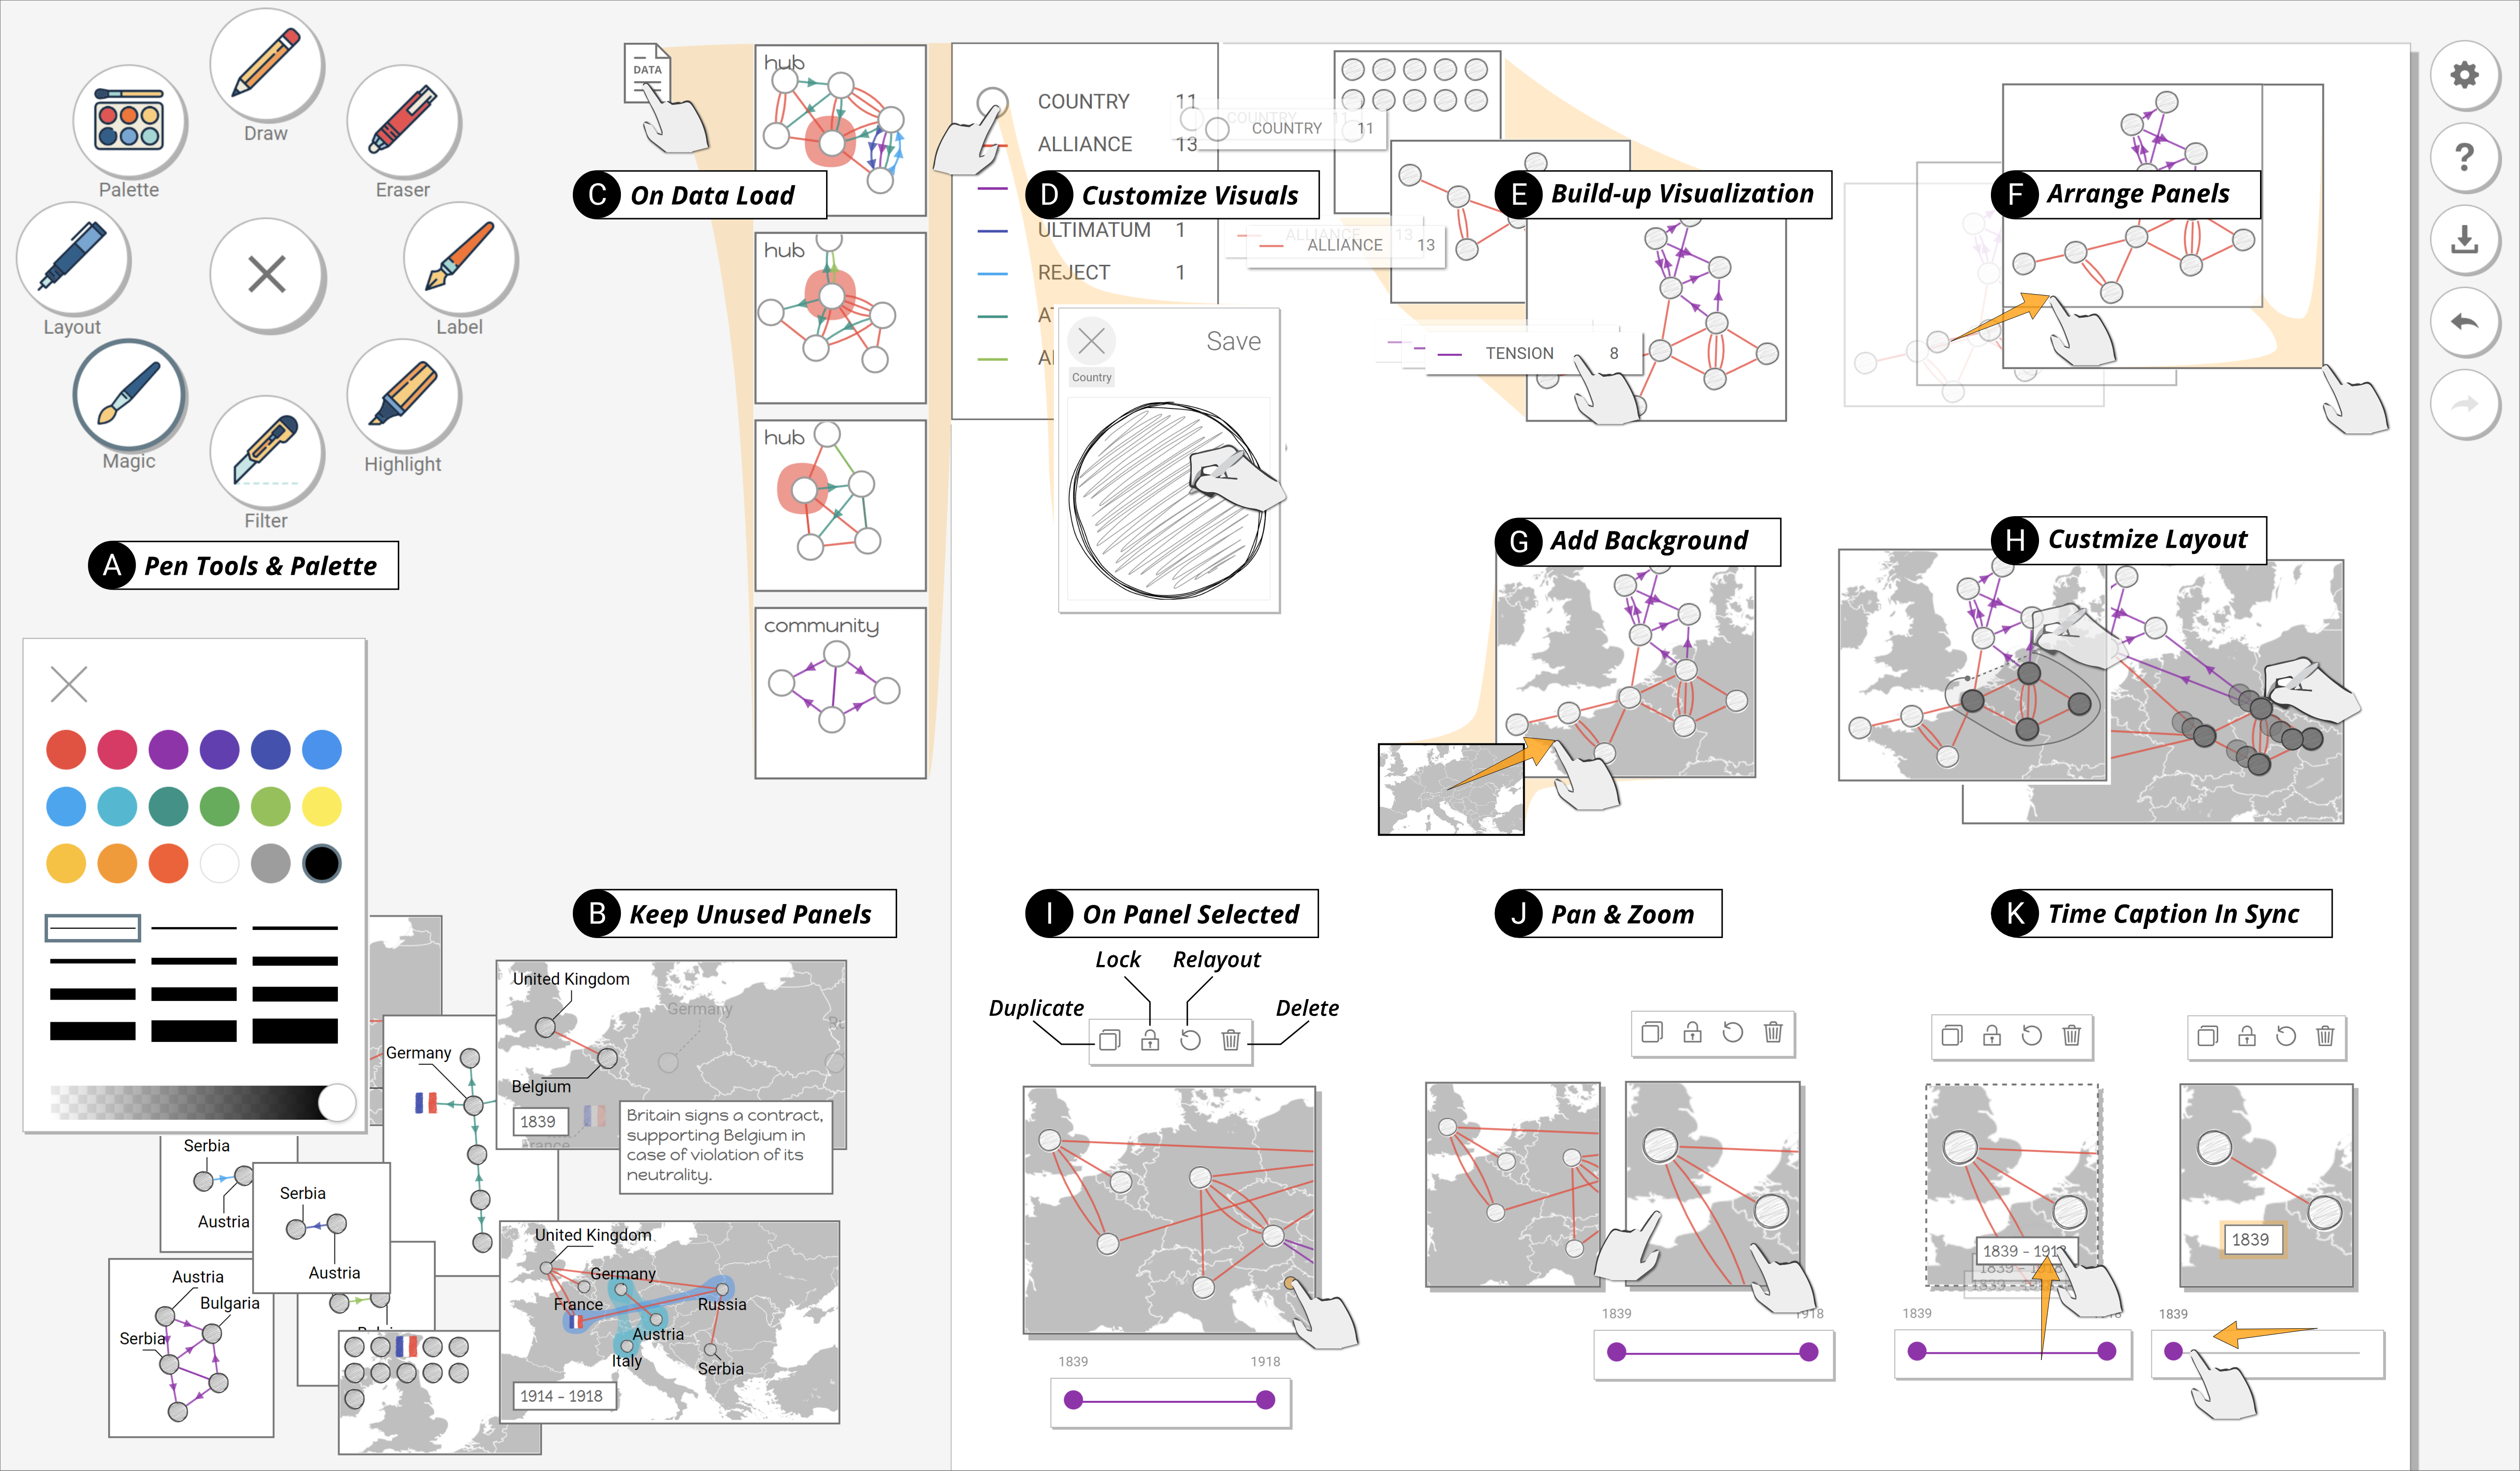
\includegraphics[width=1.0\textwidth]{figures/interface-overview.png} 
    \caption{\toolname{}'s interface: the pen can acquire different functions, such as labelling or filtering. The canvas area provides an infinite space for ideation and exploration, as well as a dedicated page area for presentation.}
    \vspace{-0.2cm}
    \label{fig:interface}
\end{figure*}

\section{Design Goals}
\label{sec:data_comics}


We conceive \toolname{} to accomplish three main goals.

\bpstart{D1. Support the creation of data \textit{comics}}
Data comics have unique characteristics and components~\cite{bach2017emerging,bachdesign}. They expose the story via a juxtaposed and sequenced panels, each containing one (or a few) insight(s). Getting the reader to focus on each insight requires that the author carefully crafts the view of each panel, such as zooming in on an important part of a network. However, identifying different characters of interest (e.g., nodes) and tracking them across panels requires that the author gives each a custom visual style to maintain consistency~\cite{qu2018keeping}. \toolname{} aims to support the crafting of panels and the expressive design of characters by direct manipulation using pen and touch, while ensuring consistency with data-driven propagation.

\bpstart{D2. Enable data-driven design}
Authoring tasks such as propagating visual designs across panels or creating transitions between panels are tedious and time-consuming. \toolname{} leverages the underlying data to automatically propagate visual designs of graphical elements and to generate textual labels and captions from data. \toolname{} also enables an author to generate transitional panels. For example, given two panels containing data at different times, \toolname{} can automatically create a series of panels representing the data at interim time points. 

\bpstart{D3. Support exploration and authoring activities}
Like any storytelling medium, the production of a comic is a creative and iterative process, often requiring the author to smoothly transition from reviewing the data and its patterns to styling them to craft a compelling story. \toolname{} facilitates the data exploration and review process by providing recommendations of interesting patterns in the data, such as a large cluster in the network, while enabling the rapid creation of visualizations using direct pen and touch manipulation. \toolname{} enables flexible workflows by providing a unique platform in which authors can review salient data aspects, rapidly generate and filter data visualizations, craft expressive visual design for data elements, compose a story by leveraging existing data comic templates, create a storyboard, or directly sequence and reorder panels. 

% 
\section{Usage Scenario}
\label{sec:scenario}

% We developed DataToon, a web-based tool for authoring data comics, based our design considerations.
To illustrate how \toolname{} accomplishes our goals and to describe key components of its interface, we describe the process taken by a hypothetical comic author named Aidan to create the comic in Figure~\ref{fig:comicbook}, adapted from Bach et al.~\cite{bach2016telling}. 

%on one appearing in the work of Bach et al. \cite{bach2016telling}.
%dynamic network dataset.
%Aiden is a high-school history teacher who wants to educate his students about the dynamics of European alliances preceding World War I. %He has experience with software like Excel and Tableau but no knowledge of graphic design software. To engage his students, he wants to use a data comic to communicate how the series of intricate alliances and conflicts evolved.
%Aidan, a high-school history teacher,  created a dataset representing a dynamic geographic and multi-faceted network where nodes are nations and links are alliances and oppositions that change over time. 



% It contains a list of European countries as nodes and alliances among the countries as links. Each alliance (i.e., link) has a temporal information about when it started and ended. 

Aidan opens \toolname{} in his web browser on a pen + touch-enabled device. The pen-tools menu (\autoref{fig:interface}A) represents the set of instruments his digital pen can acquire.  Aidan loads a dataset he previously created: a dynamic geographic and multi-faceted network containing countries and their alliances and oppositions over time. Dragging the file into the application instantiates both the legend panel and automatically generates a set of panels depicting notable structural patterns in the data (\autoref{fig:interface}C).  %Browsing legends and panels allows Aidan to recall the general content of his data. 

Aidan recalls that the evolution of alliances was interesting and he decides to explore these. He creates a new content panel by dragging the {\it Country} node type from the legend panel onto the canvas. Using the time slider for these panels (\autoref{fig:teaser}B), he filters 
\includegraphics[scale=0.02]{figures/filter_pen.png} the data back and forth to explore how the alliances changed over time. He duplicates panels as he finds interesting times, jotting down notes on them using the pencil 
\includegraphics[scale=0.02]{figures/draw_pen.png} (\autoref{fig:teaser}D).

%  he refine his ideas about the story to tell to his students. For example,

Continuing this process of exploration, Aidan now has multiple panels with annotated insights. He proceeds to craft a story for his comic by organizing them on the canvas. He wants to start with an overview of the nations involved, so he drops an image file containing a map of Europe (\autoref{fig:interface}G) into a panel, adjusting the location of each node with the \textit{Layout} pen 
\includegraphics[scale=0.02]{figures/layout_pen.png} (\autoref{fig:interface}H). He extracts country names from the data to place them on the map with the \textit{Label} pen 
\includegraphics[scale=0.02]{figures/label_pen.png}. 
%Finally, he adds a caption inside the panel to set the initial tone of the story (\autoref{fig:teaser}F).

% Once he has some idea about the narrative, he begins creating a comic strip. To show the countries in a geographic context, he loads an image showing the map of Europe (\autoref{fig:workflow}b). He wants to start by showing all the countries on the map. He uses the image as a background of the panel and positions each country node in its geographic location using the \textit{Control} pen (
\includegraphics[scale=0.05]{figures/control_pen.png}). He also creates labels to reveal the names of the countries using the \textit{Annotation} pen (
\includegraphics[scale=0.05]{figures/annotation_pen.png}). Finally, he creates a caption inside the panel to set the initial tone of the story (\autoref{fig:workflow}c).


% collecting, arranging, piling panels that may be interesting to include in the comic.

% Load image. and layout nodes in the gegraph


% He realizes the size of the panel is too small to show all the nodes, thus stretches it by dragging its right border to further right. 

After establishing the context of the story, Aidan wants to show the evolution of alliances in Europe. He reuses panels that he created earlier, transforming his rapid handwritten annotations into visual clusters around nodes, captions and labels. While he pans and zooms his first panel to emphasize two nodes (\autoref{fig:interface}J), he realizes that the difference between this panel and the first one may be too great and that his audience may fail to see the connection. He acquires the \textit{Magic} pen 
\includegraphics[scale=0.05]{figures/annotation_pen.png} to interpolate between these panels and generate intermediary ones (\autoref{fig:teaser}G). 

He generates a time caption for the last panel by dragging  the time label from the slider (\autoref{fig:interface}K, left). Duplicating this panel (\autoref{fig:interface}I) and adjusting the time automatically updates the caption (\autoref{fig:interface}K, right). Uncertain about what to show next, Aidan uses the \textit{Magic} pen 
\includegraphics[scale=0.05]{figures/annotation_pen.png} to trigger suggested panels with interesting patterns  (\autoref{fig:teaser}C). 



% He duplicates the first panel and adds the link type of \textit{Alliance} (\autoref{fig:workflow}d). He adjusts the time slider to 1839, to begin with, showing the neutrality contract % neutrality violation contract
% between the United Kingdom and Belgium. He double-taps the slider to create a caption using the current time as its text (\autoref{fig:workflow}e). 

% He lassos the two nodes to highlight, which make the rest of the countries muted into the background (\autoref{fig:workflow}f, 
\includegraphics[scale=0.05]{figures/annotation_pen.png}).

% Switching to the \textit{Control} pen (
\includegraphics[scale=0.05]{figures/control_pen.png}), he pans and zooms to set the focus of the panel to the two nodes.

As his comic nears completion, he customizes the node and link representations. For instance, he  draws a custom sketchy representation for all nodes (\autoref{fig:interface}D). To emphasize France among all countries, he paints its flag (\autoref{fig:teaser}E).
%to emphasizes the isolation of France due to the alliances of surrounding countries, he invokes the secondary canvas for the France node and
 This custom node representation is automatically propagated to all panels.  %\matt{R2's comment on the restrictiveness of data binding addresses this part of the scenario, but here is probably not the best place to discuss it} 
 Satisfied with his comic, he exports the comic as an image that he can share with his students.

% Now he wants to explain the Three Emperors alliance between Germany, Russia and Austria, which began in 1873. He again starts by duplicating the previous panel, which copies everything including the caption as well as underlying data bindings. Once he set the year to 1873 in the new panel, the time caption is automatically updated (\autoref{fig:workflow}g left). He now zooms into the three countries and highlights them into the foreground. To show the significance of the alliance, he adds a colored background to the three nodes, using the \textit{Annotation} pen but now with the pen button pressed (\autoref{fig:workflow}h).



% 
\includegraphics[scale=0.05]{figures/pencil.png}). He likes the freedom of creating his own unique style. He draws a custom, comic-like, sketchy appearance for each node by invoking a contextualized canvas from the legend panel (\autoref{fig:workflow}i). He similarly draws a country flag for France by lassoing its node using \textit{Pencil} (
\includegraphics[scale=0.05]{figures/pencil.png}) with the pen button pressed. These custom visuals are automatically propagated to all other panels. Before finishing, he saves the current comic strip as an image to see if it looks good in print.



% He create a series of panels and jot down a node on each panel on what to show 



% 1. Top-down 

% starting with story boarding. create empty panels, layout them, write down notes, etc.

% 2. Bottom up

% create a detailed panel, copy and paste progressively.





% \begin{figure*}[!t]
%     \centering
% 	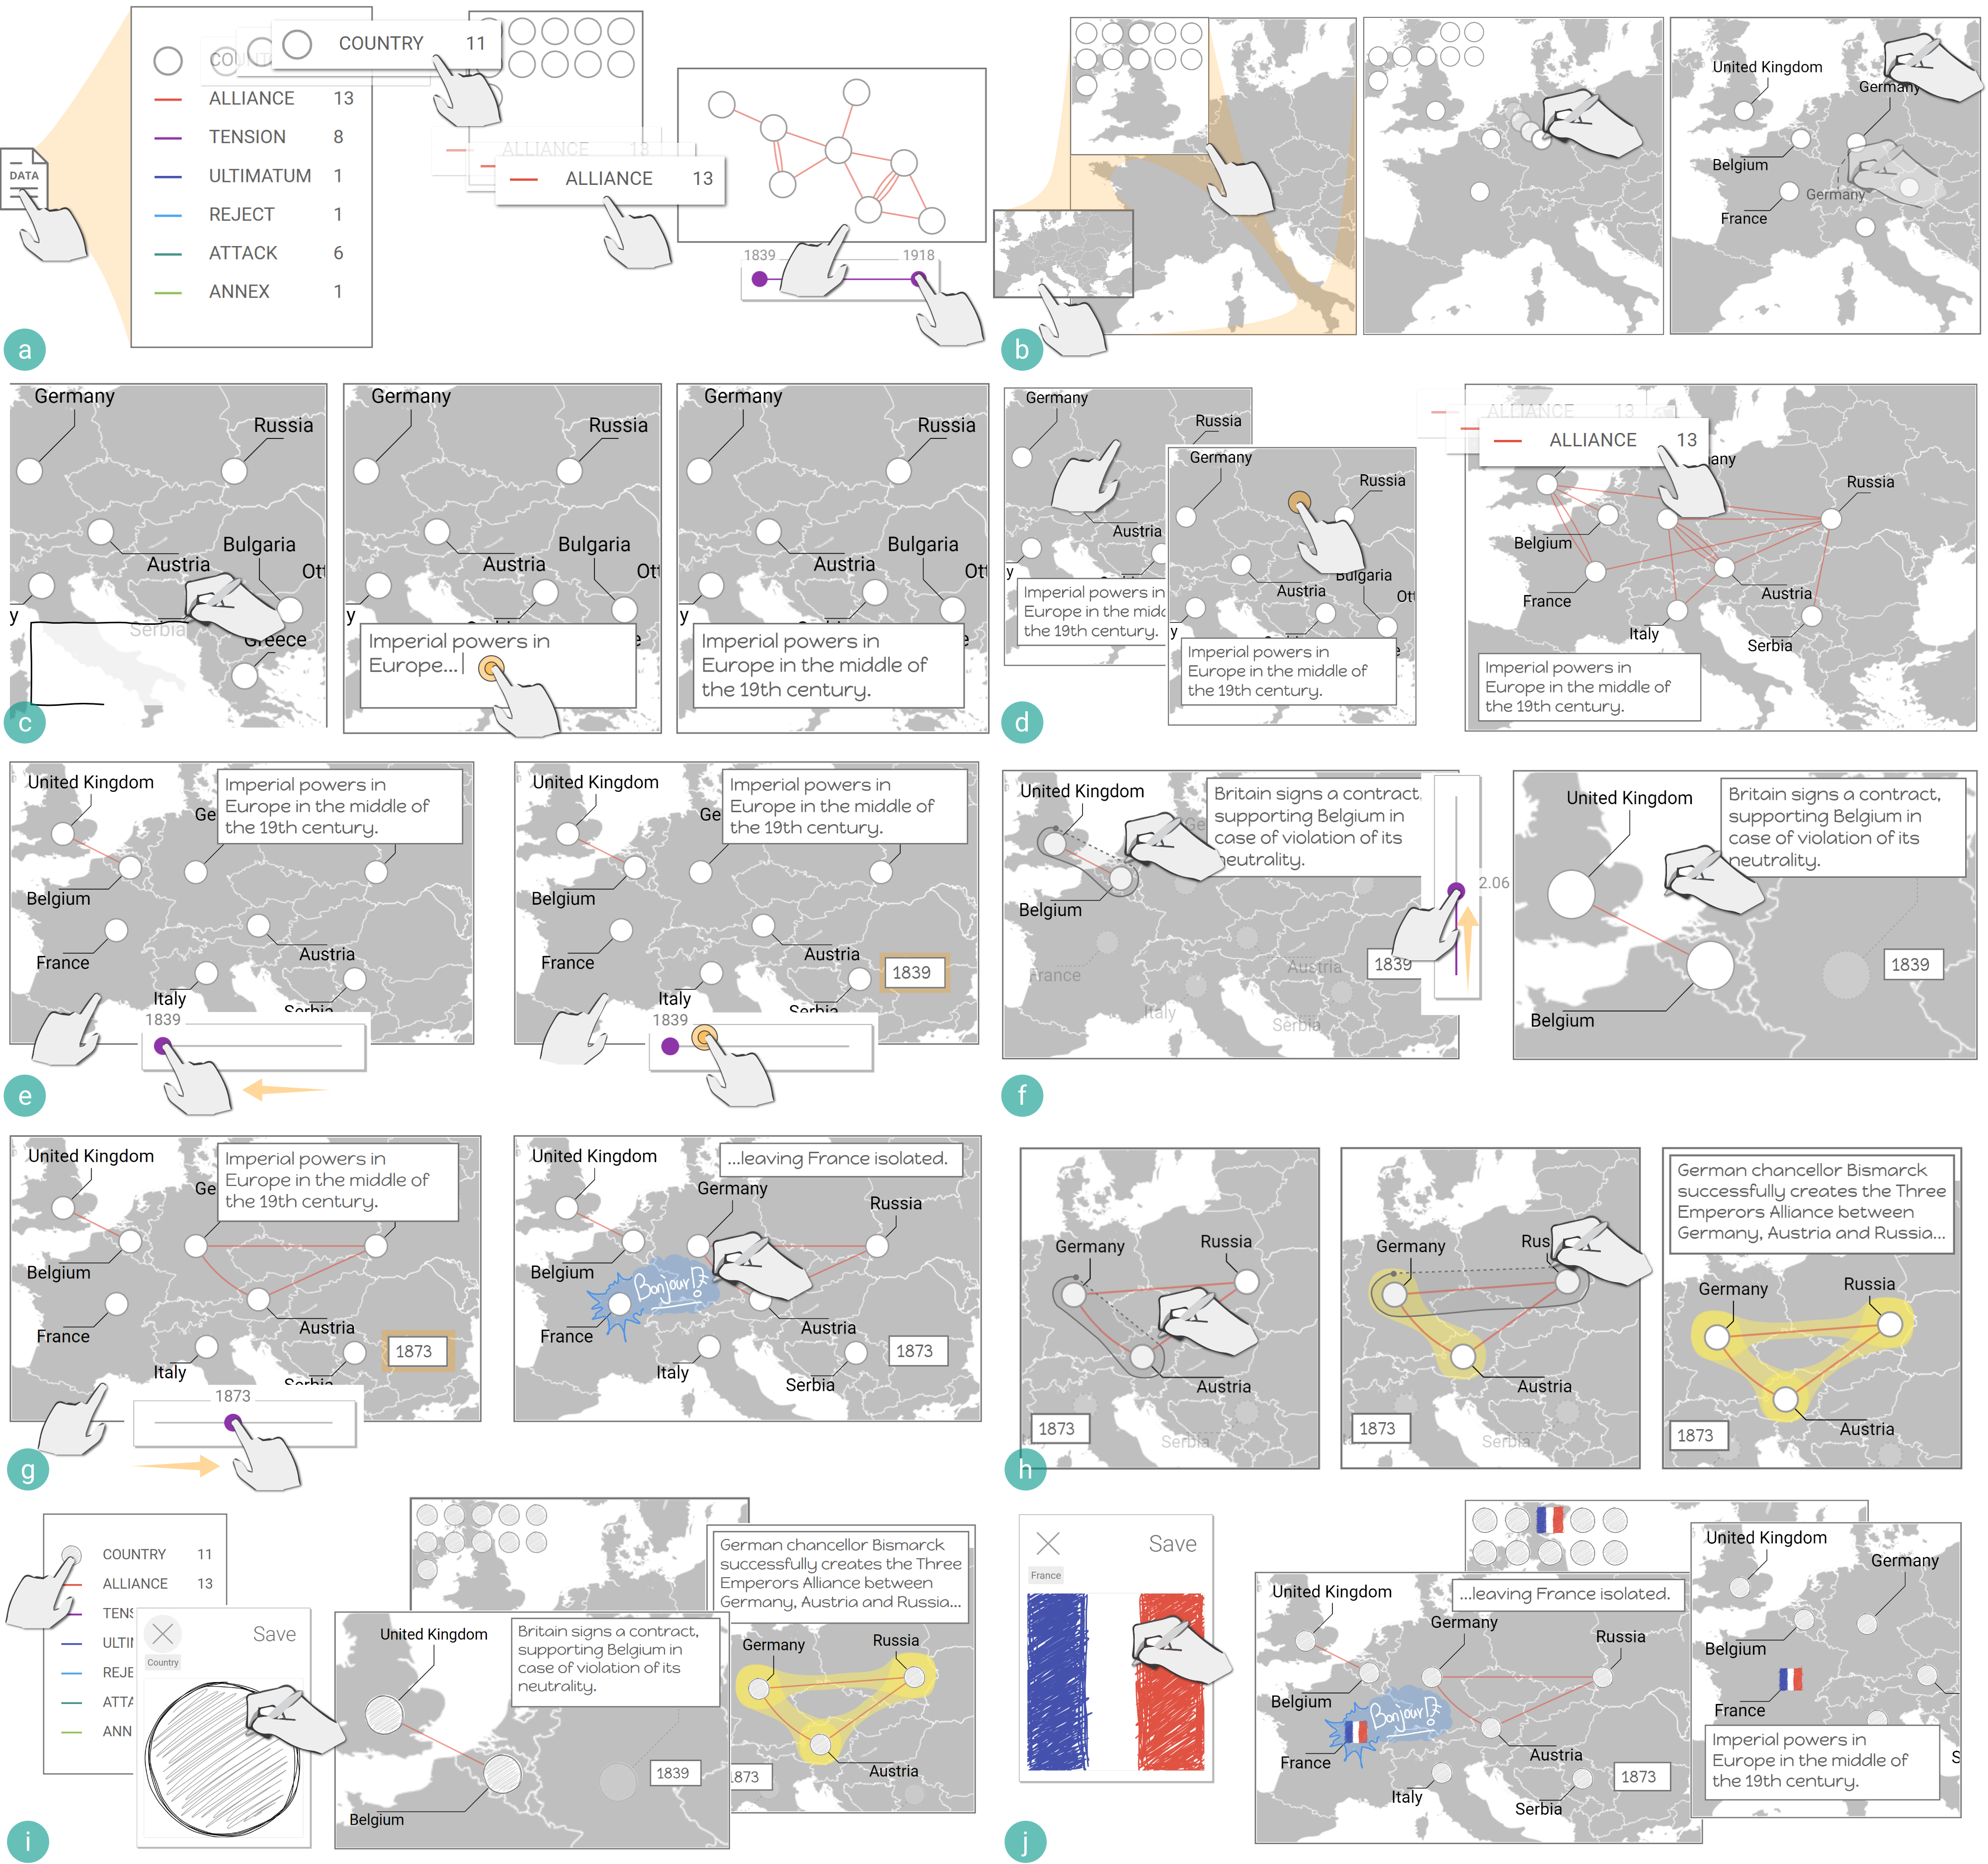
\includegraphics[width=\textwidth]{figures/workflow_full} 
% 	\caption{The workflow of creating the data comic described in \autoref{sec:workflow} and shown in \autoref{fig:tool_overview}. (a) importing a dataset to create the legend panel and fluidly exploring the data through simple drag and drop and the time slider. (b) importing a background image, laying out nodes, and creating labels. (c) creating a caption by drawing a rectangle and double-tapping it to edit its text. (d) duplicating the panel through hold and tap, and incrementally adding additional data to the panel. (e) filtering data using the time slider and creating a time caption by double-tapping it. (f) lassoing nodes to show in the foreground and panning and zooming through the combination of pen and touch. (g) updating the time caption automatically and adding a freeform annotation through sketching. (h) Creating a highlighted group. (i) the contextual canvas allows the author to sketch new visual mappings for all country nodes and for (j) France specifically.}
%     \vspace{-0.2cm}
%     % \caption{\rev{Five} examples of data comics created using \toolname{}}
%     \label{fig:workflow}
% \end{figure*}

% \begin{figure*}[!t]
% 	\subfigure[]
% 	{
% 	   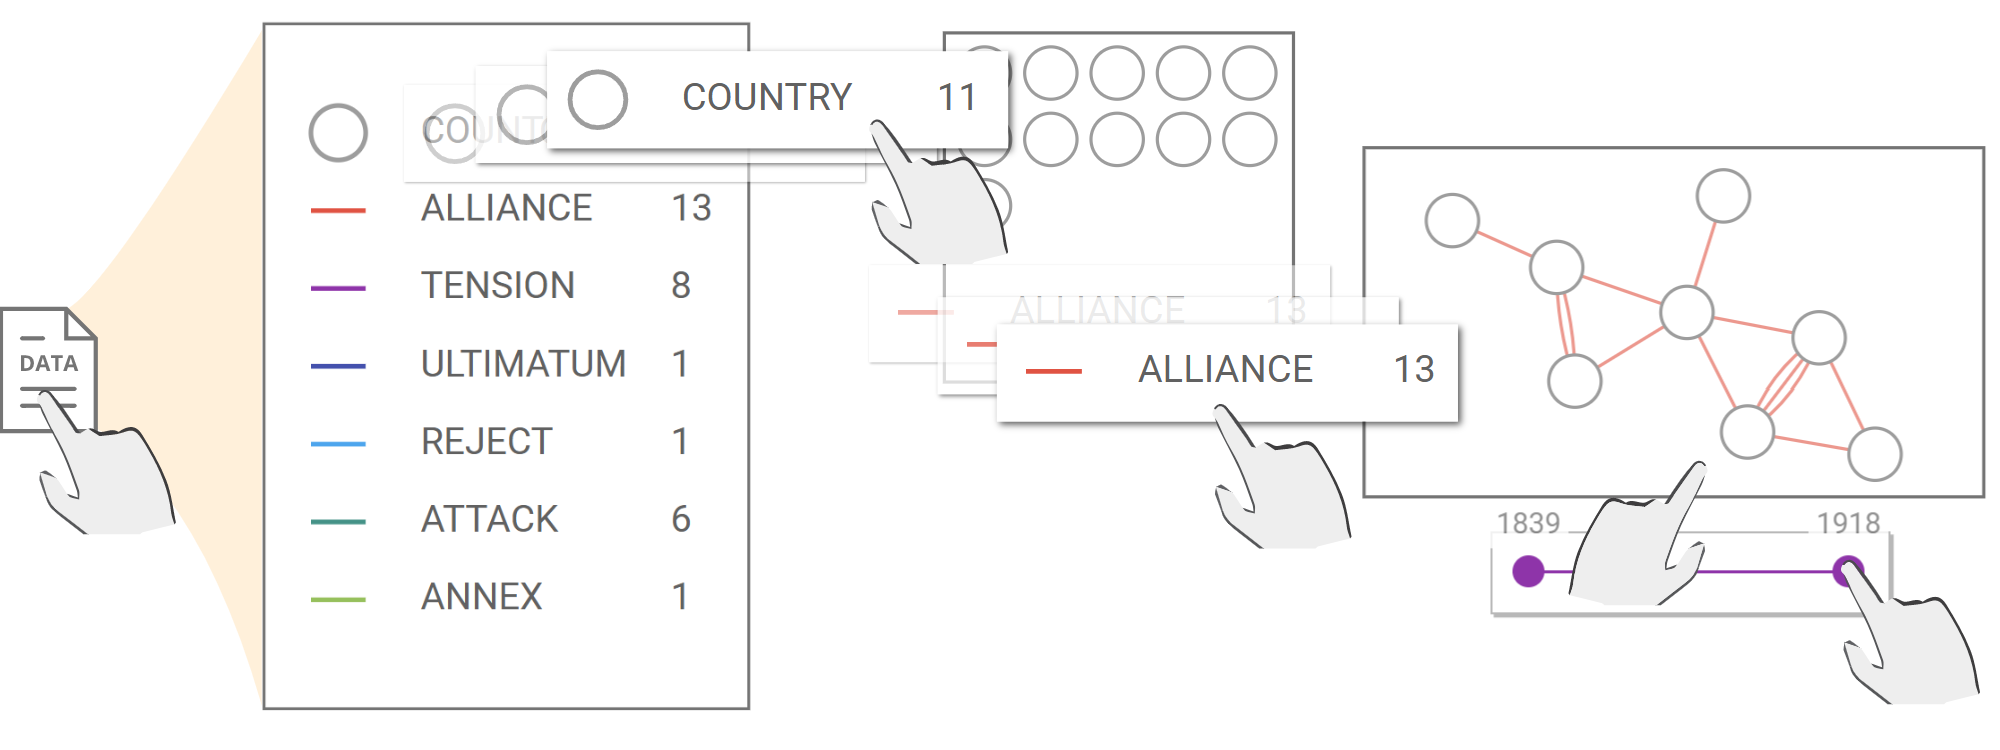
\includegraphics[width=1\columnwidth]{figures/workflow1}
% 		\label{fig:workflow1}
% 	}
% 	\hfill
% 	\subfigure[]
% 	{
% 	   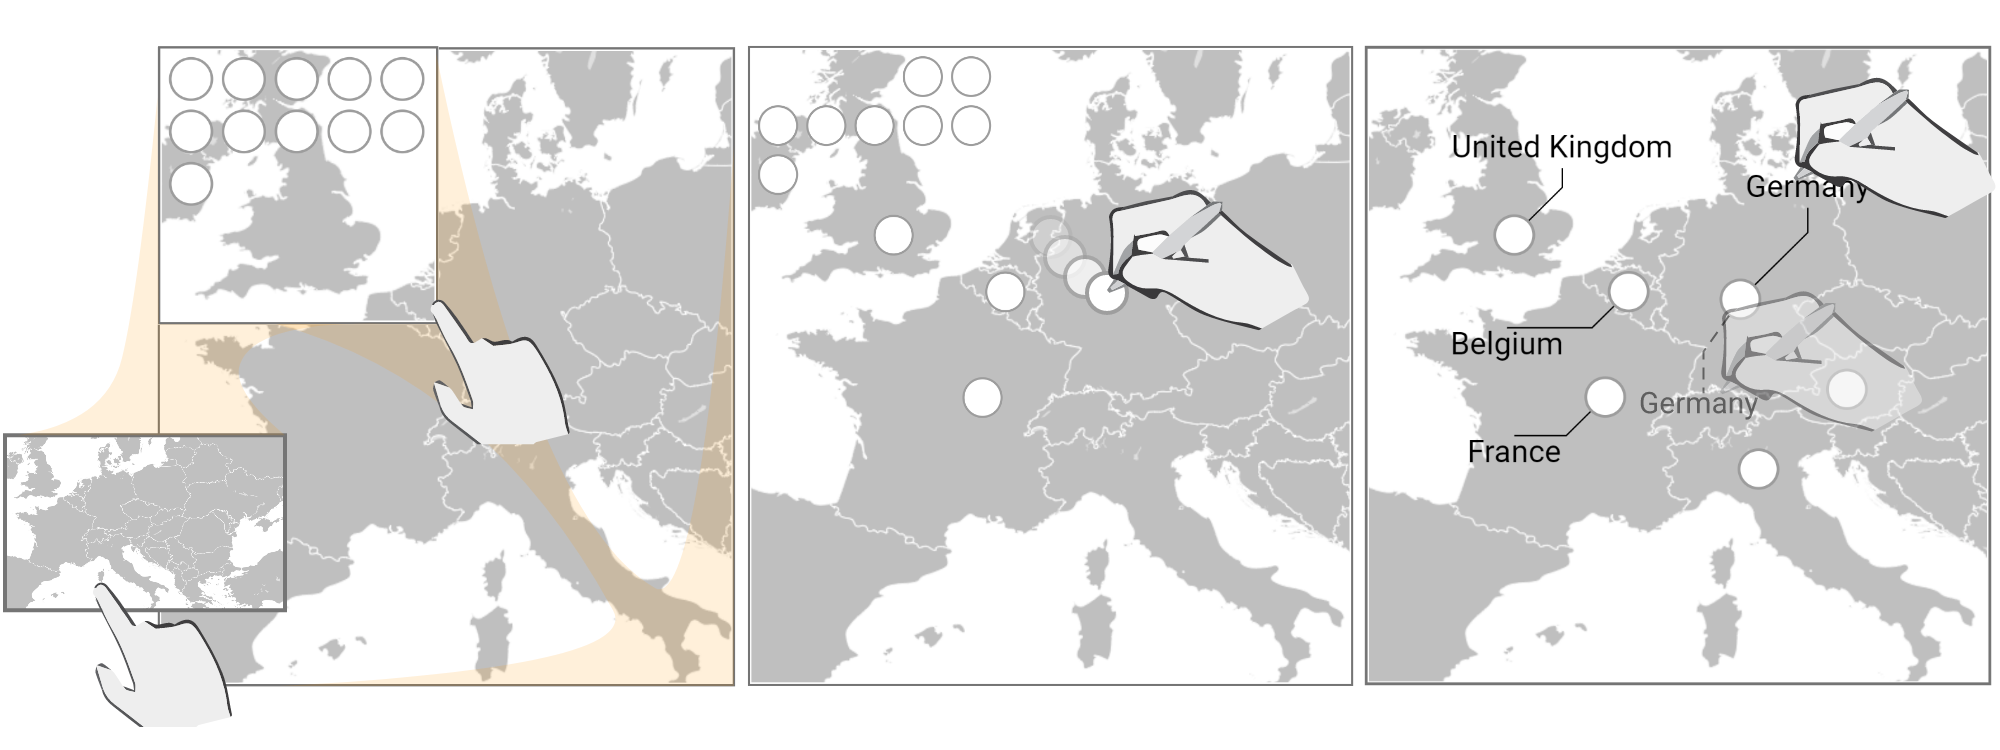
\includegraphics[width=1\columnwidth]{figures/workflow2}
% 		\label{fig:workflow2}
% 	}
% 	\hfill
% 	\subfigure[]
% 	{
% 		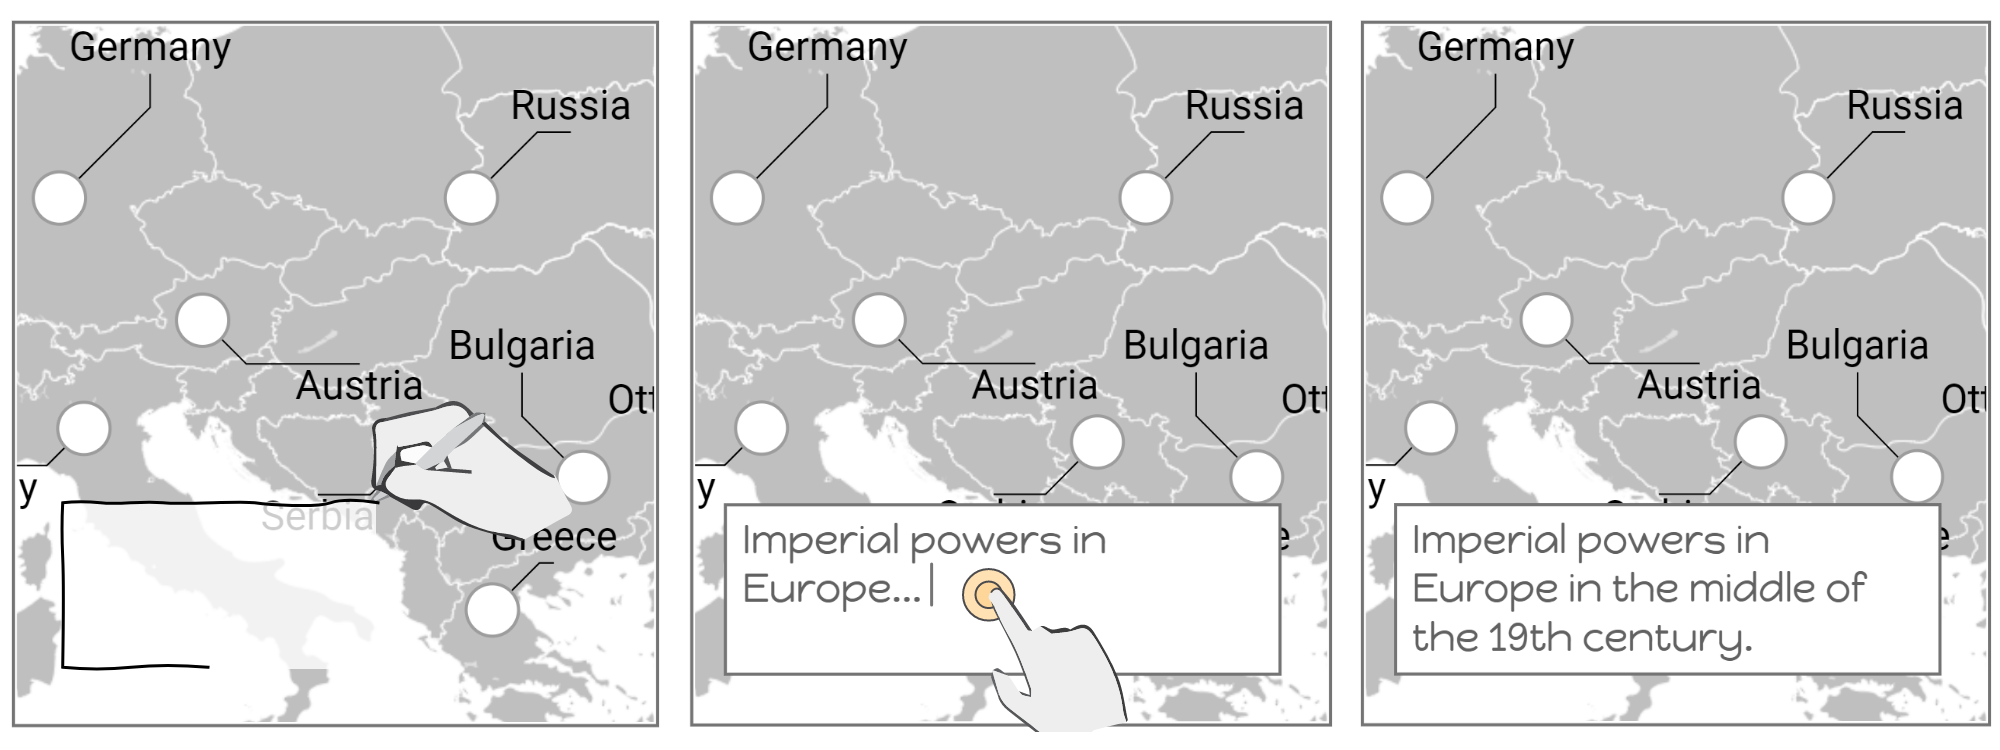
\includegraphics[width=1\columnwidth]{figures/workflow3}
% 	   \label{fig:workflow3}
% 	}
% 	\hfill
% 	\subfigure[]
% 	{
% 	   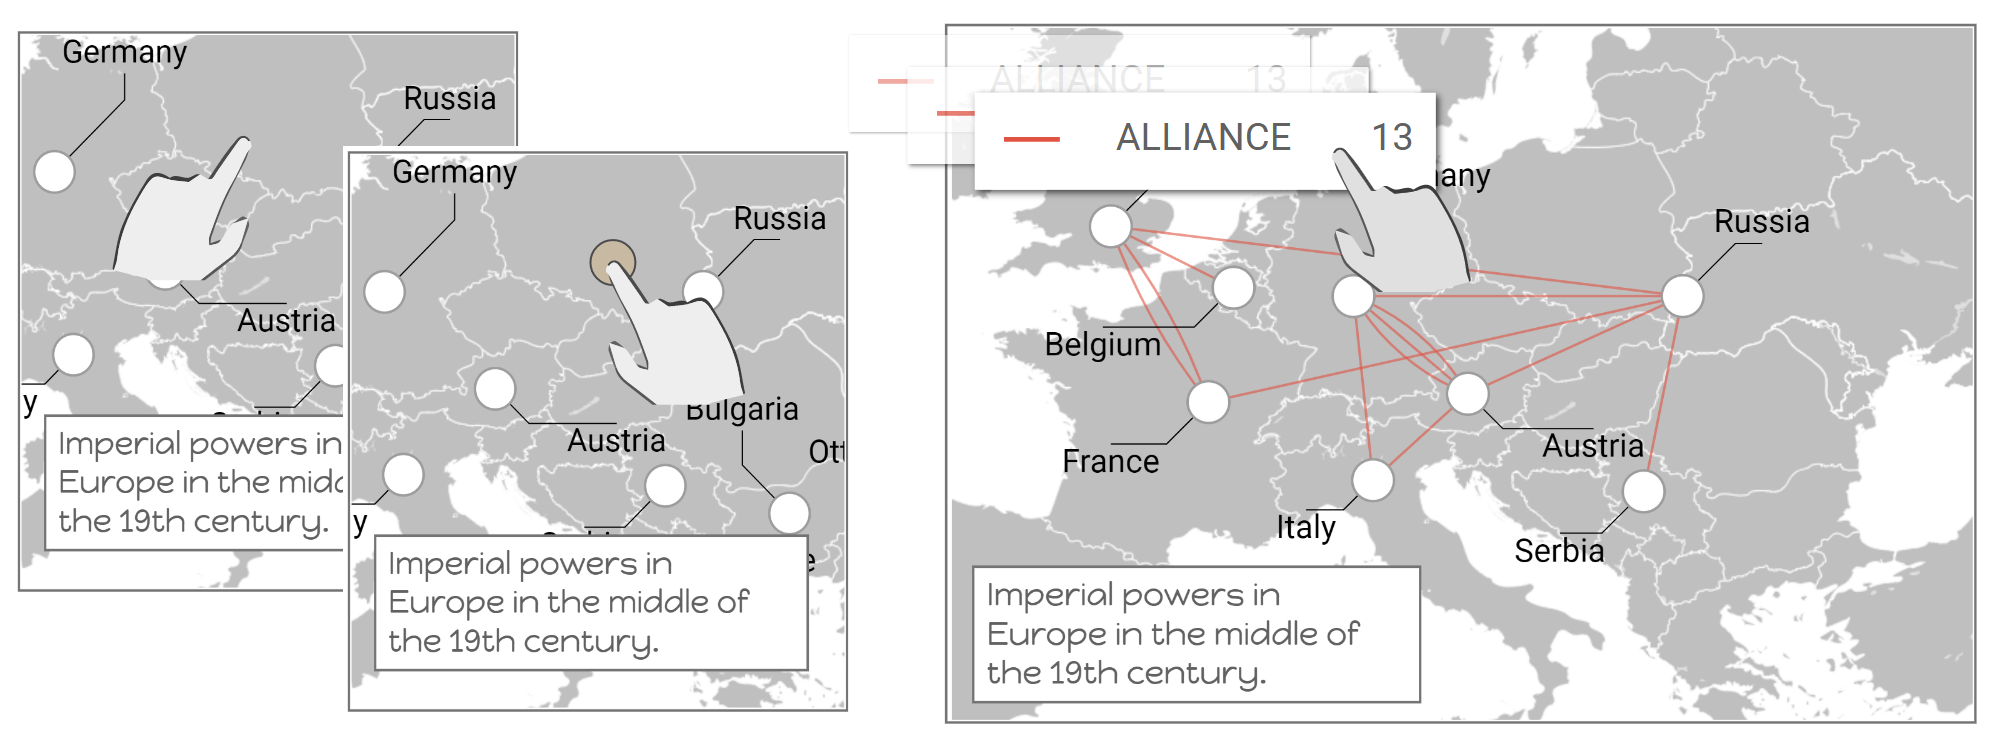
\includegraphics[width=1\columnwidth]{figures/workflow4}
% 		\label{fig:workflow4}
% 	}
% 	\hfill
% 	\subfigure[]
% 	{
% 		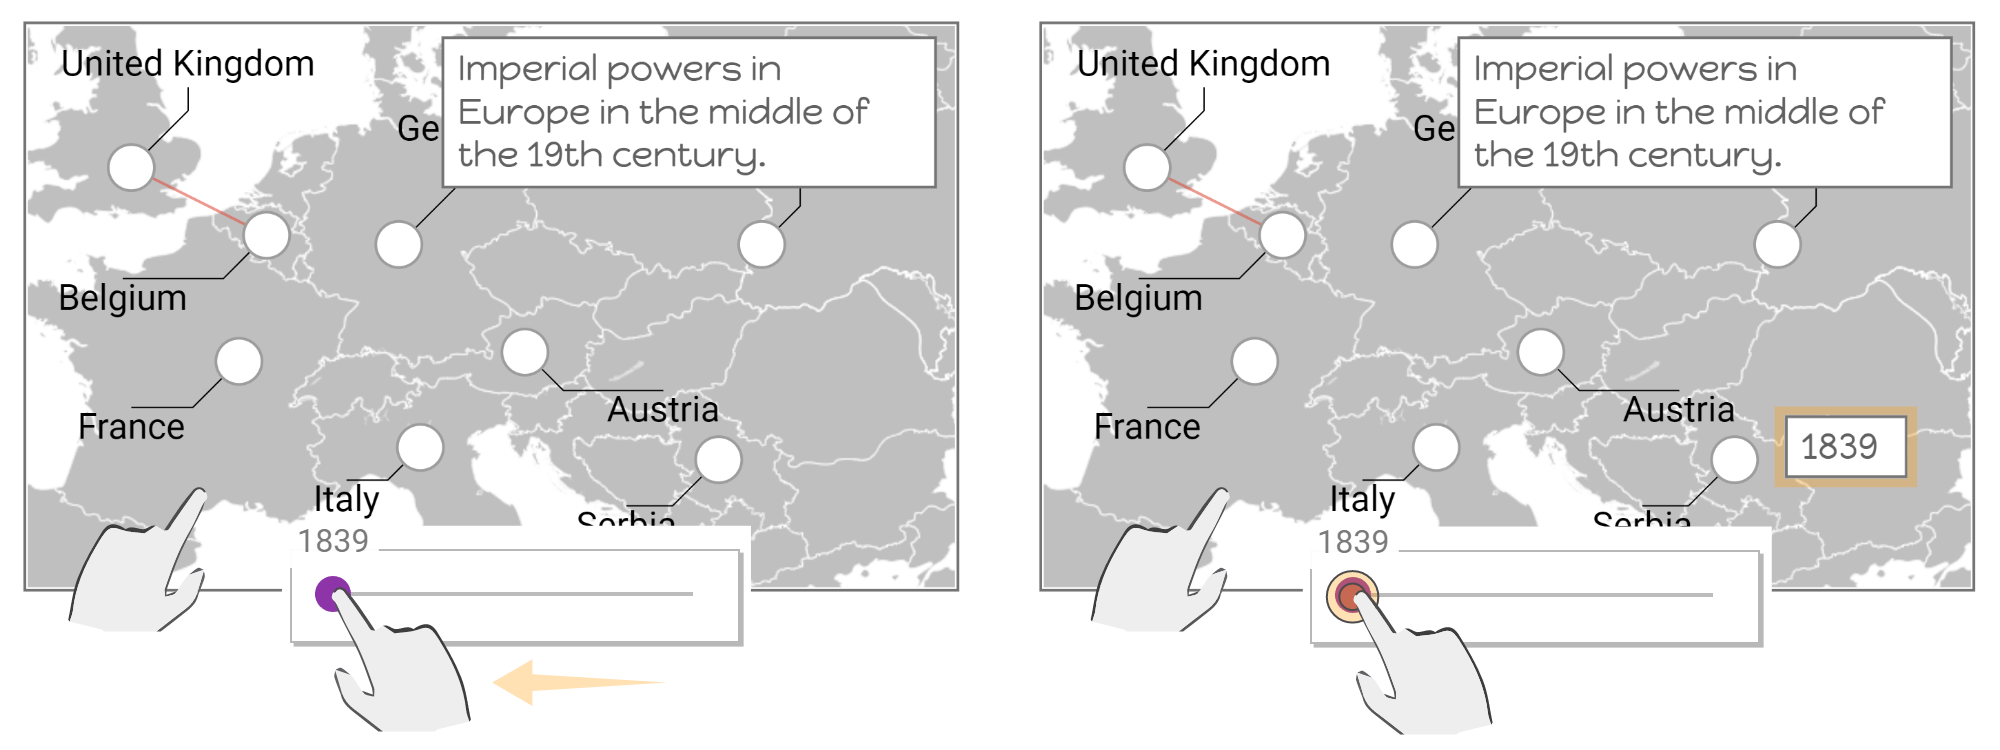
\includegraphics[width=1\columnwidth]{figures/workflow5}
% 		\label{fig:workflow5}
% 	}
% 	\hfill
% 	\subfigure[]
% 	{
% 		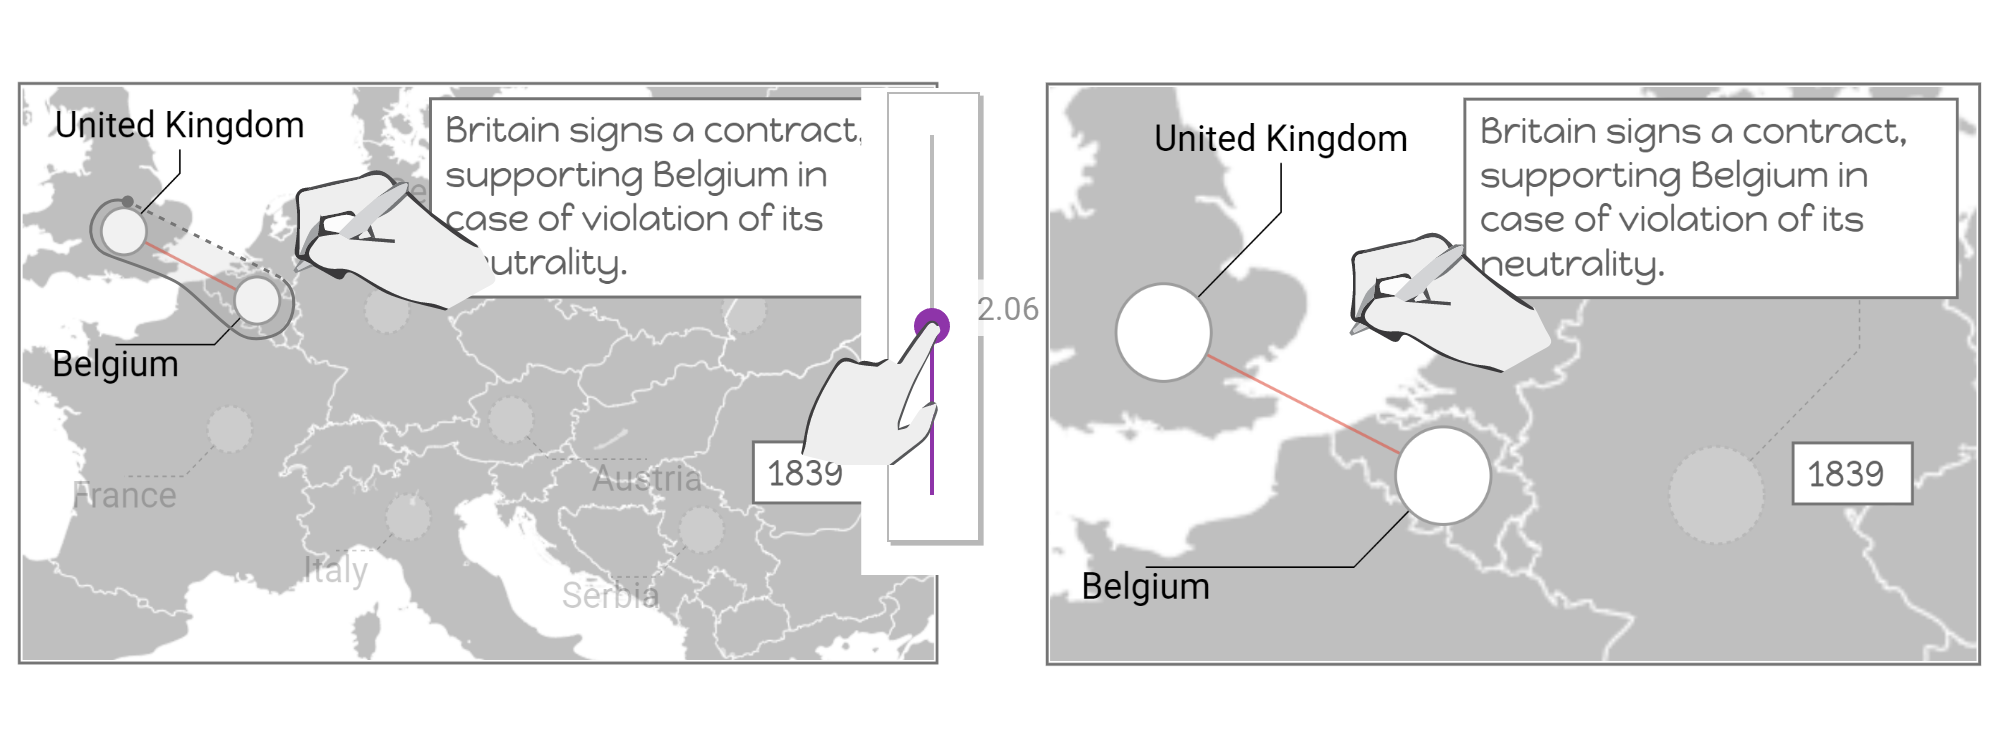
\includegraphics[width=1\columnwidth]{figures/workflow6}
% 		\label{fig:workflow6}
% 	}
% 	\hfill
% 	\subfigure[]
% 	{
% 		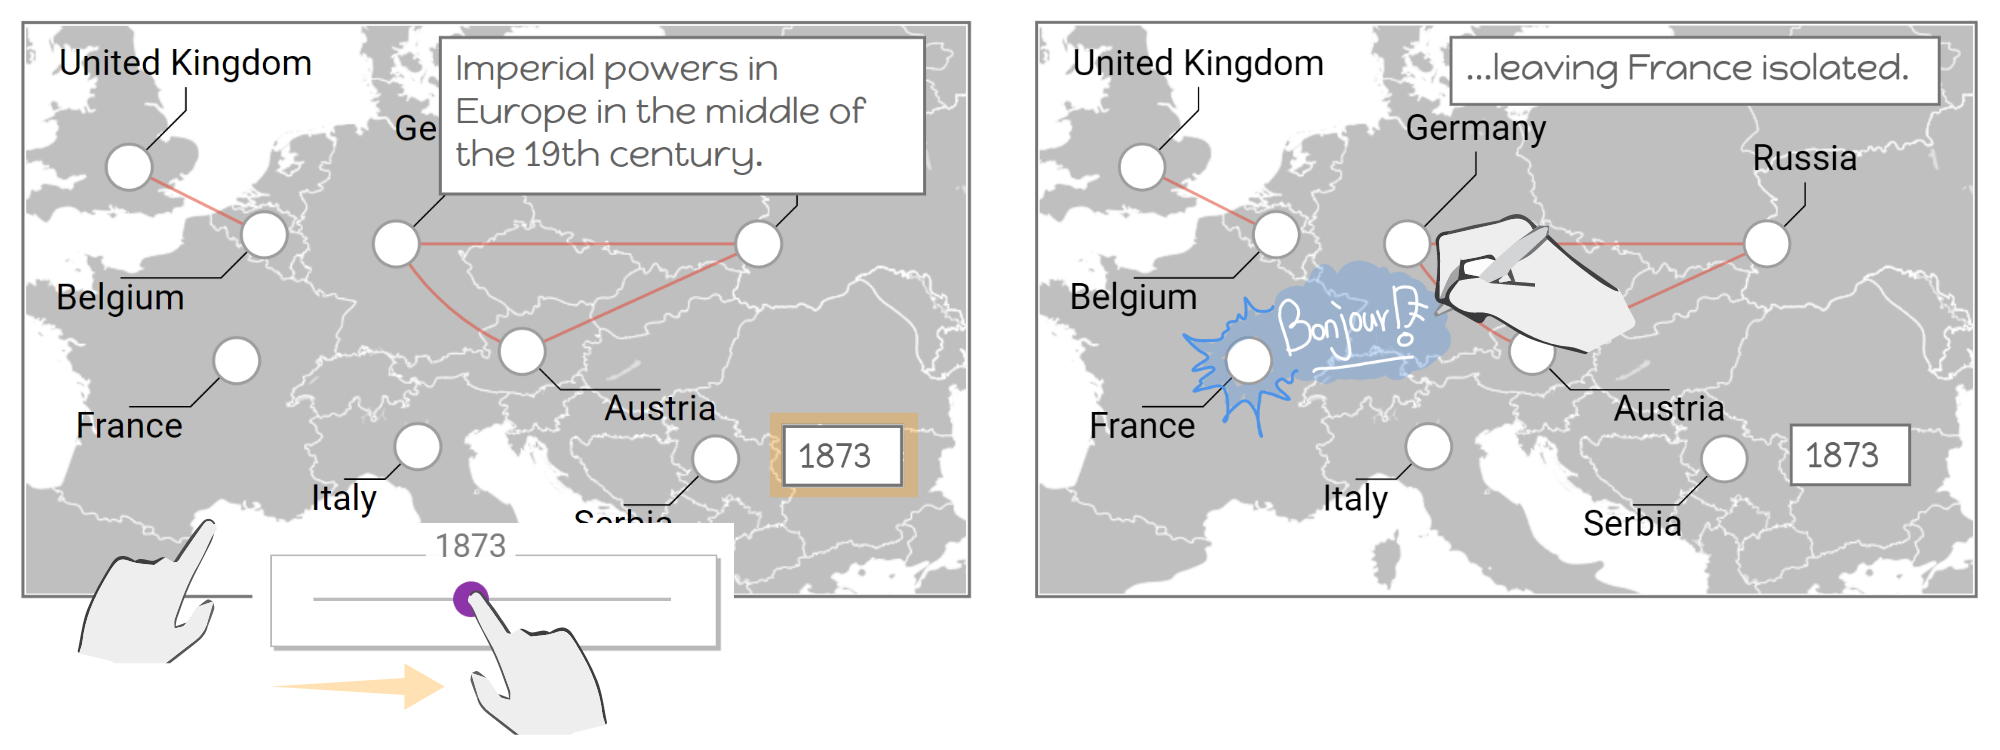
\includegraphics[width=1\columnwidth]{figures/workflow7}
% 		\label{fig:workflow7}
% 	}
% 	\hfill
% 	\subfigure[]
% 	{
% 		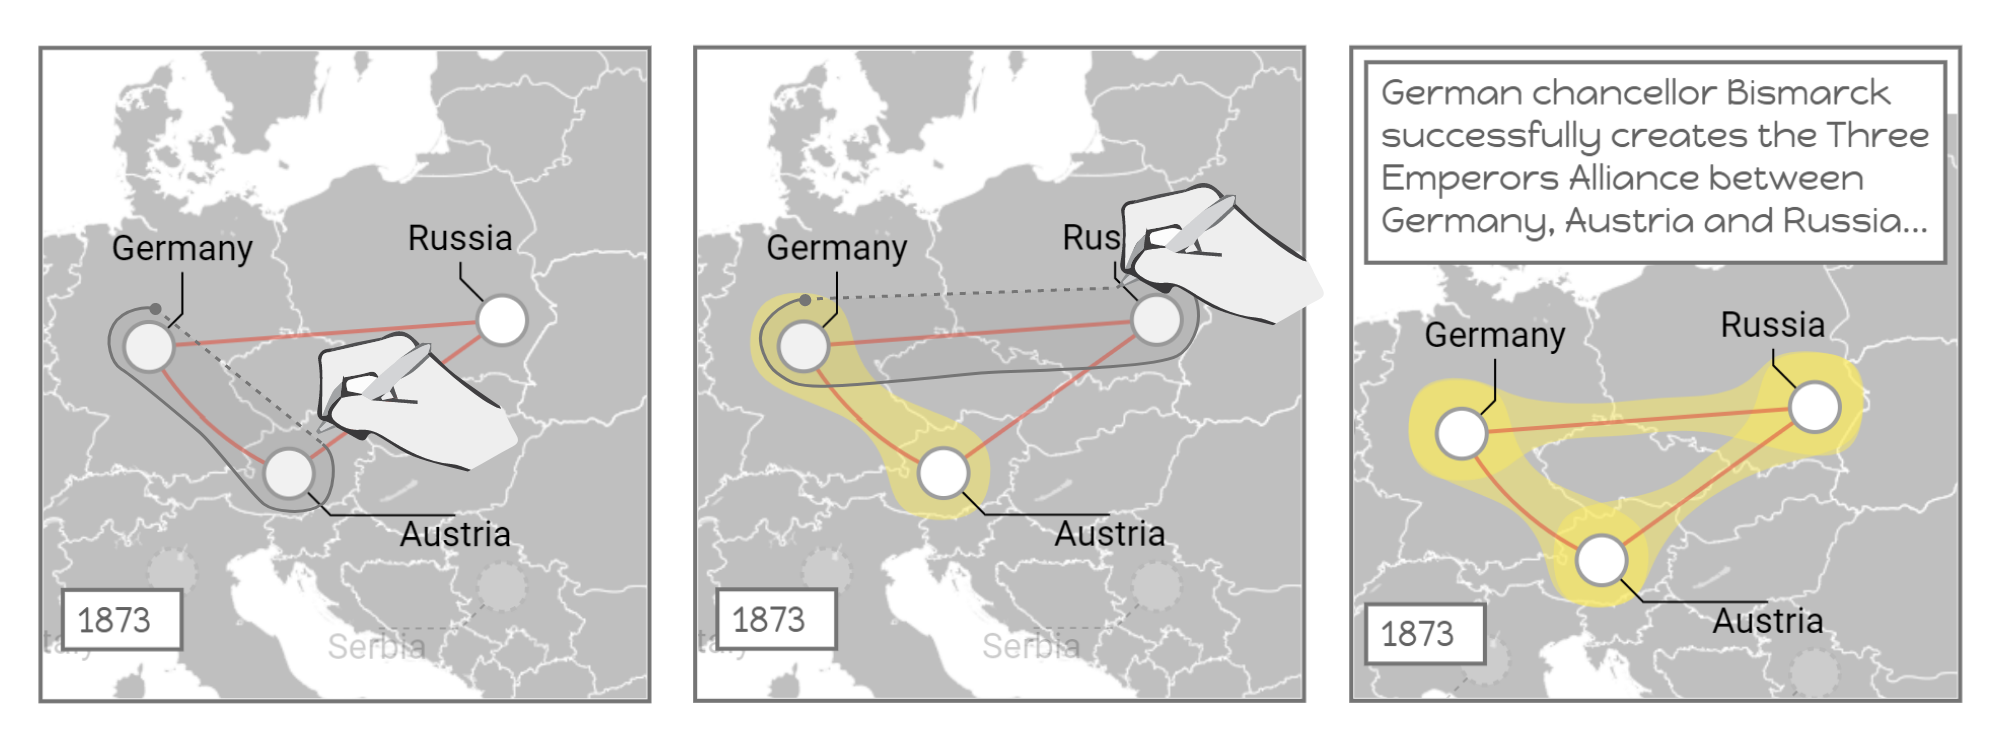
\includegraphics[width=1\columnwidth]{figures/workflow8}
% 		\label{fig:workflow8}
% 	}
% 	\hfill
% 	\subfigure[]
% 	{
% 		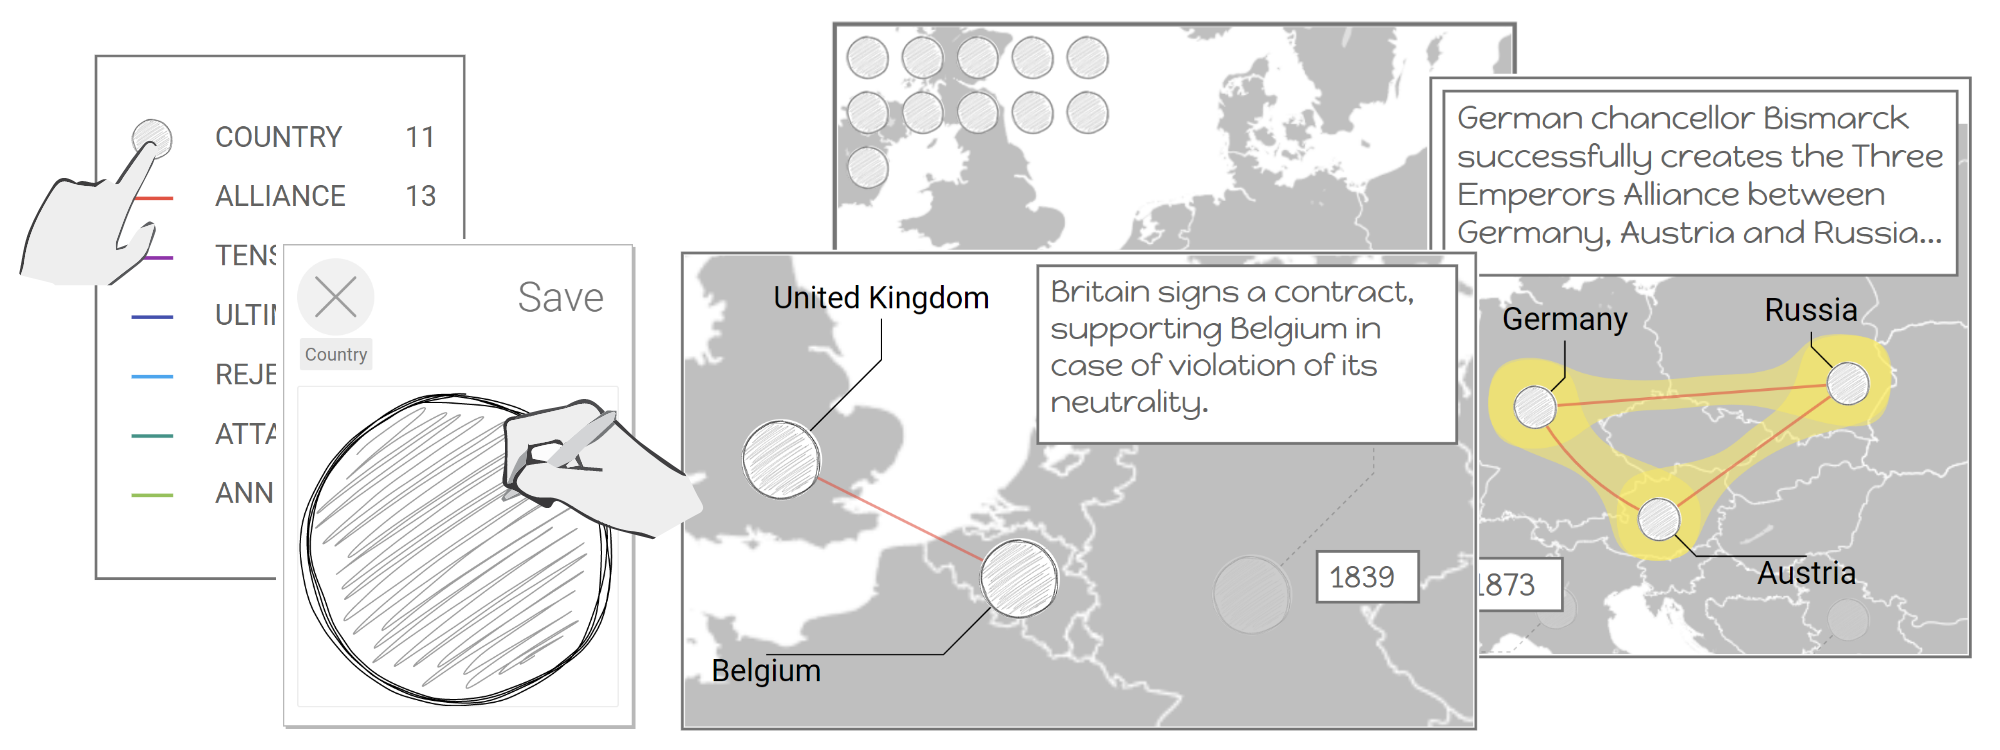
\includegraphics[width=1\columnwidth]{figures/workflow9}
% 		\label{fig:workflow9}
% 	}
% 	\hfill
% 	\subfigure[]
% 	{
% 		\includegraphics[width=1\columnwidth]{figures/workflow10}
% 		\label{fig:workflow10}
% 	}
%    \caption{The workflow of creating the data comic described in \autoref{sec:workflow} and shown in \autoref{fig:tool_overview}. (a) Importing a dataset to create the legend panel and fluidly exploring the data through simple drag and drop and the time slider. (b) Importing a background image, laying out nodes, and creating labels. (c) creating a caption by drawing a rectangle and double-tapping it to edit its text. (d) Duplicating the panel through hold and tap, and incrementally adding additional data to the panel. (e) Filtering data using the time slider and creating a time caption by doube-tapping it. (f) Lassoing nodes to show in the foreground and panning and zooming through the combination of pen and touch. (g) Updating the time caption automatically and adding a freeform annotation through sketching. (h) Creating a highlighted group. (i) Updating a visual mapping for all country nodes. (j) Updating a visual mapping for France. }
%    \label{fig:workflow}
%    \end{figure*}

% 
\begin{figure*}[!tbp]
    \centering
    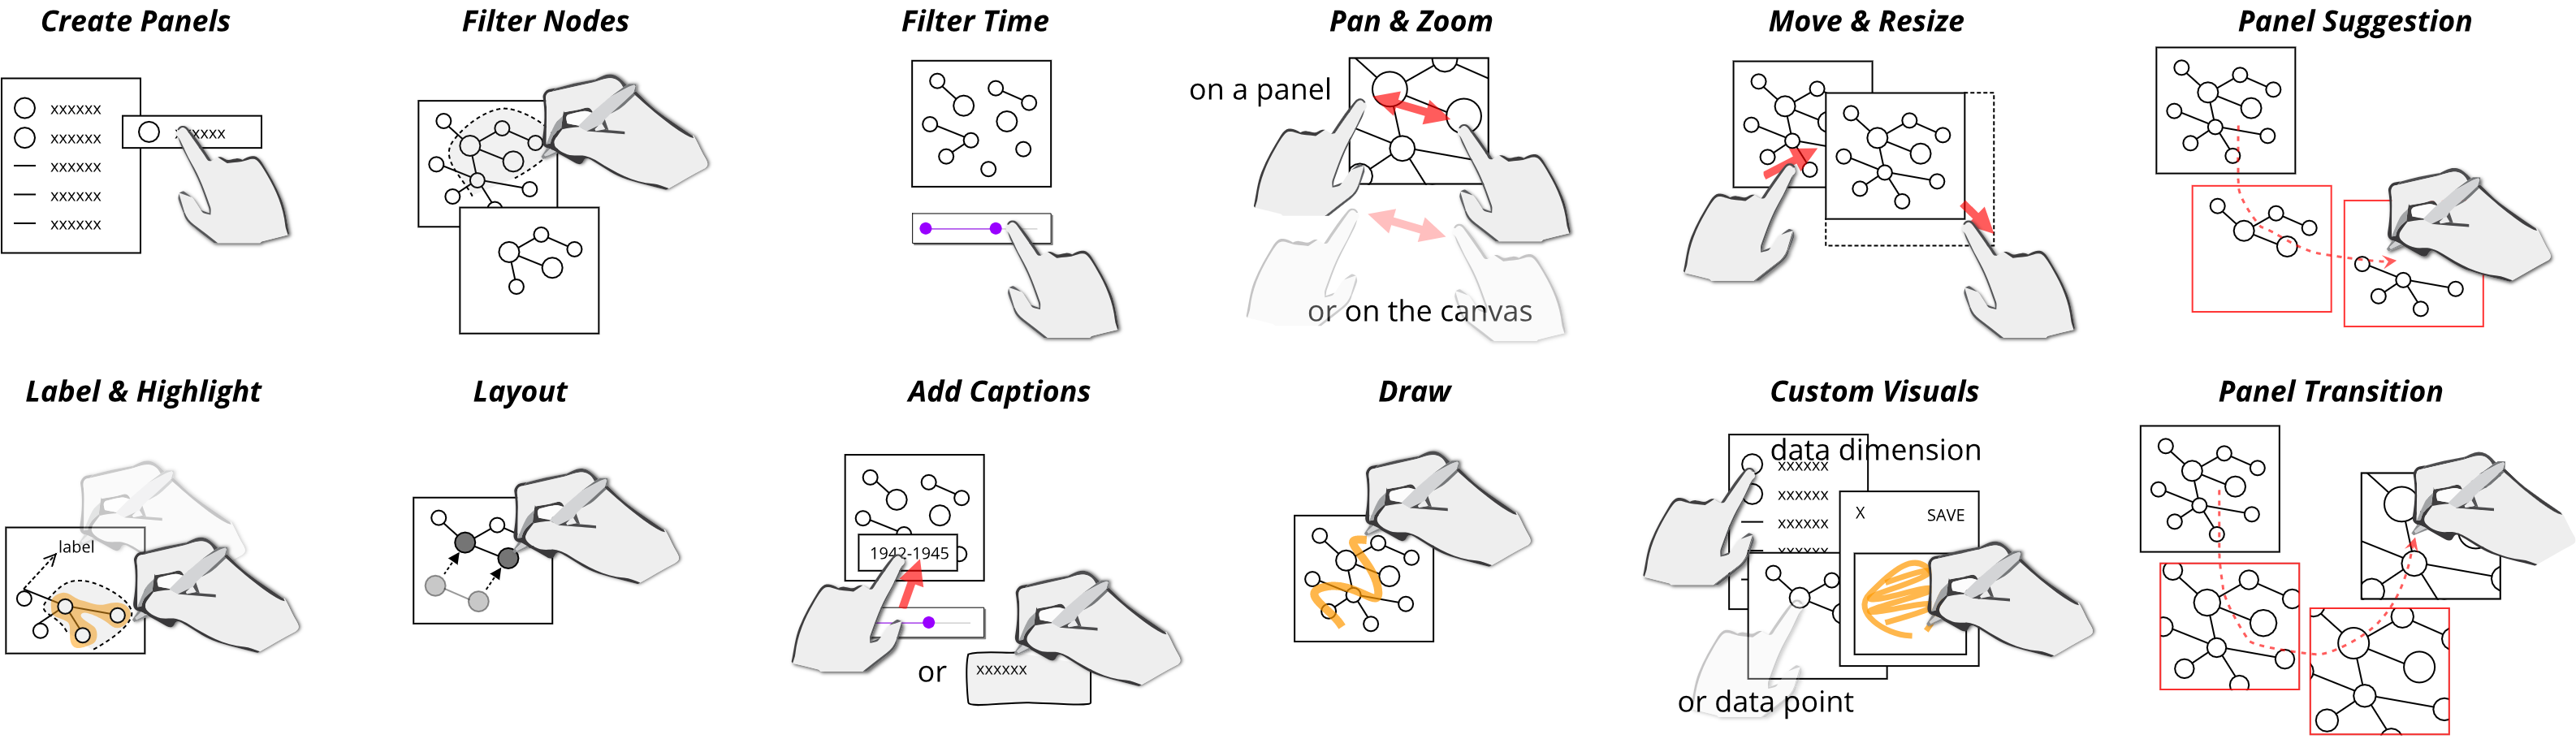
\includegraphics[width=1.0\textwidth]{figures/interaction.png} 
    % \vspace{-0.4cm}
    \caption{An overview of the pen + touch interactions supported by \toolname{}.}
	\label{fig:interaction}
    % \vspace{-0.4cm}
\end{figure*}

\section{\toolname{}}
\label{sec:datatoon}

We designed \toolname{} for a broad range of people who wish to craft data comics that communicate insights about their data. This may include graphic designers without programming expertise, data analysts without design expertise tasked with communicating their findings, or educators seeking new ways to engage their students. %\matt{trying to relate this to our scenario and study participants}
% This sections describes \toolname{}'s interface and its pen + touch interactions. %\matt{section feels too long, too user-manual-esque}

\subsection{Data Abstraction}
%\matt{Promoting this paragraph based on R3's comments, though I haven't commented on network size limitations}
As mentioned in the introduction, we chose to focus on dynamic network data since it is poorly supported by existing communicative visualization and storytelling tools, and because of its inherent parallel to the dynamic interactions between characters appearing in comics.   
In particular, \toolname{} supports multivariate dynamic network data, which consists of nodes and links and their attributes. A node can have a label and a type, as well start and end dates. A link must have source and target nodes and may have a direction and a weight along with same set of attributes describing nodes. Given this criteria, \toolname{} also supports static networks, where neither nodes nor links have associated start or end times. Note that \toolname{} is primarily a storytelling tool, one suitable for communicating different aspects of dynamic network data; we do not address scalability issues and analysis tasks related to very large networks in this paper. 
  
\subsection{Story Abstraction}

Like a comic book, a data comic consists of pages (\autoref{fig:comicbook}), in which each page can contain multiple panels. A panel is the essential building block of a narrative structure, which can in turn contain visualization, images, text captions, and annotation.
% The relationship between panels is defined by their spatial positions that are often further complicated through varying sizes of the panels. 
The spatial arrangement of panels having varying size and content generates a unique narrative flow, enabling a nonlinear reading experience unlike linear sequences produced by other storytelling tools. 
% \matt{reuse the following later?}
% DataToon uses a comic book metaphor, allowing the author to create multi-page comics . Each page can embed a separate dataset, if necessary, to show a different facet of the story.
% The author can export each page into an image for printing and sharing. 
% Data filters, including type, temporal and node filters, and view transforms control the content of the panels, namely visualizations; that is, the underlying data is shared and reused across the panels so as mappings for custom visuals. Narration to highlight important aspects of the data or to convey data-driven messages is accomplished through the annotations. 

% A visual data story much relies on the elements of comics, integrated with data-driven abstractions. The model mainly consists of multiple panels, visualizations within the panels, and data-driven, visual and textual annotations. Panels are building blocks of a narrative structure. 

% focused tool set, data binding, rapid prototyping

% To allow people to craft expressive data representations (C1) as well as experiment with panel layout composition (C4), we opted to design \toolname{} as a pen+touch application. We reasoned that sketching afforded by the pen would stimulate creative and expressive designs, while direct touch interactions would encourage authors to experiment with panel arrangements.
%data comics via bimanual direct manipulation pen and touch interactions, overcoming the challenges described in \autoref{sec:data_comics}. 

\subsection{Interaction Design}

% The \toolname{} interface offers a focused set of instruments (materialized by different modes of use of the pen) to enable the creation, editing and styling of multiple panels representing different aspects of the data and experiment with their organization in space (materialized by a set of manipulable views on a zoomable canvas). 
\toolname{} is comprised of a canvas for storyboarding; content and legend panels for presenting visual representations of data; a set of pen tools for content creation and manipulation; and a contextual canvas for sketching custom visuals.

%that are contextually relevant to the elements of a data comic, from panels and pages to visualizations and annotations.
% A key aspect of \toolname{}'s design is to support data binding across panels, enabling functionality that other applications do not support, such as automatically propagating changes of visual representations to other panels to maintain consistency (C2) and automatically generating transitions between two panels (C3). % that have no connection to the underlying data.
% By combining a focused tool set with data binding, \toolname{} allows for rapid iterative design of data comics that could only be achieved via laborious manual efforts today.

% \subsection{User Interface}
% \toolname{} has a few main user interface components (\autoref{fig:tool_overview}). The page canvas (\autoref{fig:tool_overview}d) provides an authoring environment for managing visualization panels and drawing freeform annotations. The legend panel (\autoref{fig:tool_overview}d, upper left) not only shows the overview of visual mappings but also serves as an interface for creating content. The contextual canvas (\autoref{fig:workflow}i,j) is invoked on demand from the legend for customizing visual mappings, e.g., for sketching custom icons for nodes. The pen tool menu (\autoref{fig:tool_overview}a) allows the author to switch between functions from sketching to annotation and transition.
  
  
\autoref{fig:interaction} summarizes our pen + touch interactions. In general, our interaction design choices reflect the mantra: \textit{the pen writes, touch manipulates}~\cite{hinckley2010pen}. However, since individual nodes and links within panels are often too small to manipulate with a finger, the pen is also used to manipulate visual elements in some circumstances, as described below.  Throughout the interface, we chose to visually expose interactive controls rather than rely on implicit multi-touch gestures that are difficult to discover and remember. Note that we describe our final system, which improves upon the version used in our reproduction study described below.

% \matt{redundant}
% where touch always manipulates panels such moving and resizing). By default, the pen writes (
\includegraphics[scale=0.025]{figures/draw_pen.png}) but acquires different tools depending on the selected pen type (
\includegraphics[scale=0.025]{figures/label_pen.png} 
\includegraphics[scale=0.025]{figures/highlight_pen.png} 
\includegraphics[scale=0.025]{figures/filter_pen.png}  
\includegraphics[scale=0.025]{figures/magic_pen.png}  
\includegraphics[scale=0.025]{figures/layout_pen.png}). 


% In addition, visualization usually consists of a multitude of data points, making it cumbersome to manipulate using fingers.


% We made this design decision because a visualization usually consists of a multitude of data points, making it cumbersome to manipulate using fingers.

% It is cumbersome to manipulate the content mostly consisting of a fine-grained elements of a visualization. Thus, we decided to use the pen, instead of fingers, as a primary mode of interaction for the panel content. The pen acquires different functions depending on the pen type.  The pen eraser deletes the type of visual elements created through the pen type. 

% a list of node types and link types in the dataset. The pen tool menu allow users to acquire different pen functions applied to panels. A side menu for additional features such as undoing and redoing changes and importing the page to an external image file. (png and svg). 

\vspace{2mm}
\bpstart{Interacting with the canvas} 
\toolname{} provides an infinite canvas to support flexible authoring and rapid ideation, transitioning from data exploration to authoring activities (D3). The author can navigate the canvas via pan and zoom gestures. Meanwhile, using the pen, the author can draw or write anywhere on the canvas, either to annotate content or to add storyboarding notes and ideas. The author can create an empty panel by simply drawing a rectangle, to be filled later with content, or create panels from data. Panels can be freely arranged and resized with touch interactions, leading to different layouts at any point in the authoring process. 

%Our design decision for providing a flexible authoring environment is to allow for multiple workflows and fluidity in the iterative design process, while sketching can further amplify the expressive capability of such an environment due to its inherent informality % freeform and effortless nature
% \cite{xia2018dataink}.
\vspace{2mm}
\bpstart{Interacting with the legend panel}
A legend panel is created when the author drags a dataset file onto the canvas. This panel provides an overview of the dynamic network, displaying a list of node types and link types along with the cardinality of each type. 
%It plays a vital role in helping readers understand the visual encodings to the underlying data. 
%The author can import a dataset by dragging a data file onto the canvas (\autoref{fig:workflow}a). It causes a legend panel to appear, providing an overview of the dataset
This legend also serves as an interface for creating content panels. Dragging a node or link type from the legend onto the canvas creates a new content panel displaying a filtered visualization of the data. Dragging a node type automatically creates a unit chart of all nodes in the data matching this type. Dragging a link type automatically creates a force-directed node-link diagram of nodes connected by this link type. Note that links can convey both weight and direction via line thickness and arrows, should these optional attributes be provided. 

Node and link types can also be dragged from the legend panel to an existing content panel, whereupon its contents are updated to reflect the additional type (\autoref{fig:interface}E) and its layout recomputed. For instance, dragging a link type to a content panel containing a unit chart will convert the chart into a node-link diagram. Similarly, adding a link type to a panel containing a node-link diagram will generate multiple link types (see Figure~\ref{fig:interface}). 
% The core content of the panel is a visualization created from the legend panel. The number of data dimensions added to the panel determines the type and complexity of the visualization within. For example, multiple node types create a stacked unit chart , while having at least one link type generates a node-link diagram. Each node and link can use its shape size and line thickness respectively to encode a weight, while the link can additionally encode its direction (i.e., a simplified multivariate network). 
% The latter action is akin to adding a data filter to the panel. 
\vspace{2mm}

\bpstart{Interacting with content panels}
A content panel may contain visualizations, text, annotations, a background image, or some combination thereof (D1). Panels can  be nested: drawing a rectangle inside a panel creates a child panel, which is useful for text captions or inset visualizations. 
It is possible to duplicate an existing panel, copying all of the content of the source panel to a new panel (\autoref{fig:interface}I). This interaction is particularly useful for progressively building a narrative using the previous panel as a starting point.

Tapping on a panel containing a visualization selects it and enables panning and zooming within the panel. This also reveals a time slider for the panel, which applies additional temporal filtering to nodes and links displayed within the panel. Dragging this slider onto the panel creates a nested time caption panel (D2), which remains updates as the user changes the time slider (\autoref{fig:interface}K). 

%\matt{I forgot about this interaction. It doesn't seem very discoverable} 

\begin{figure}[b]
    \centering
    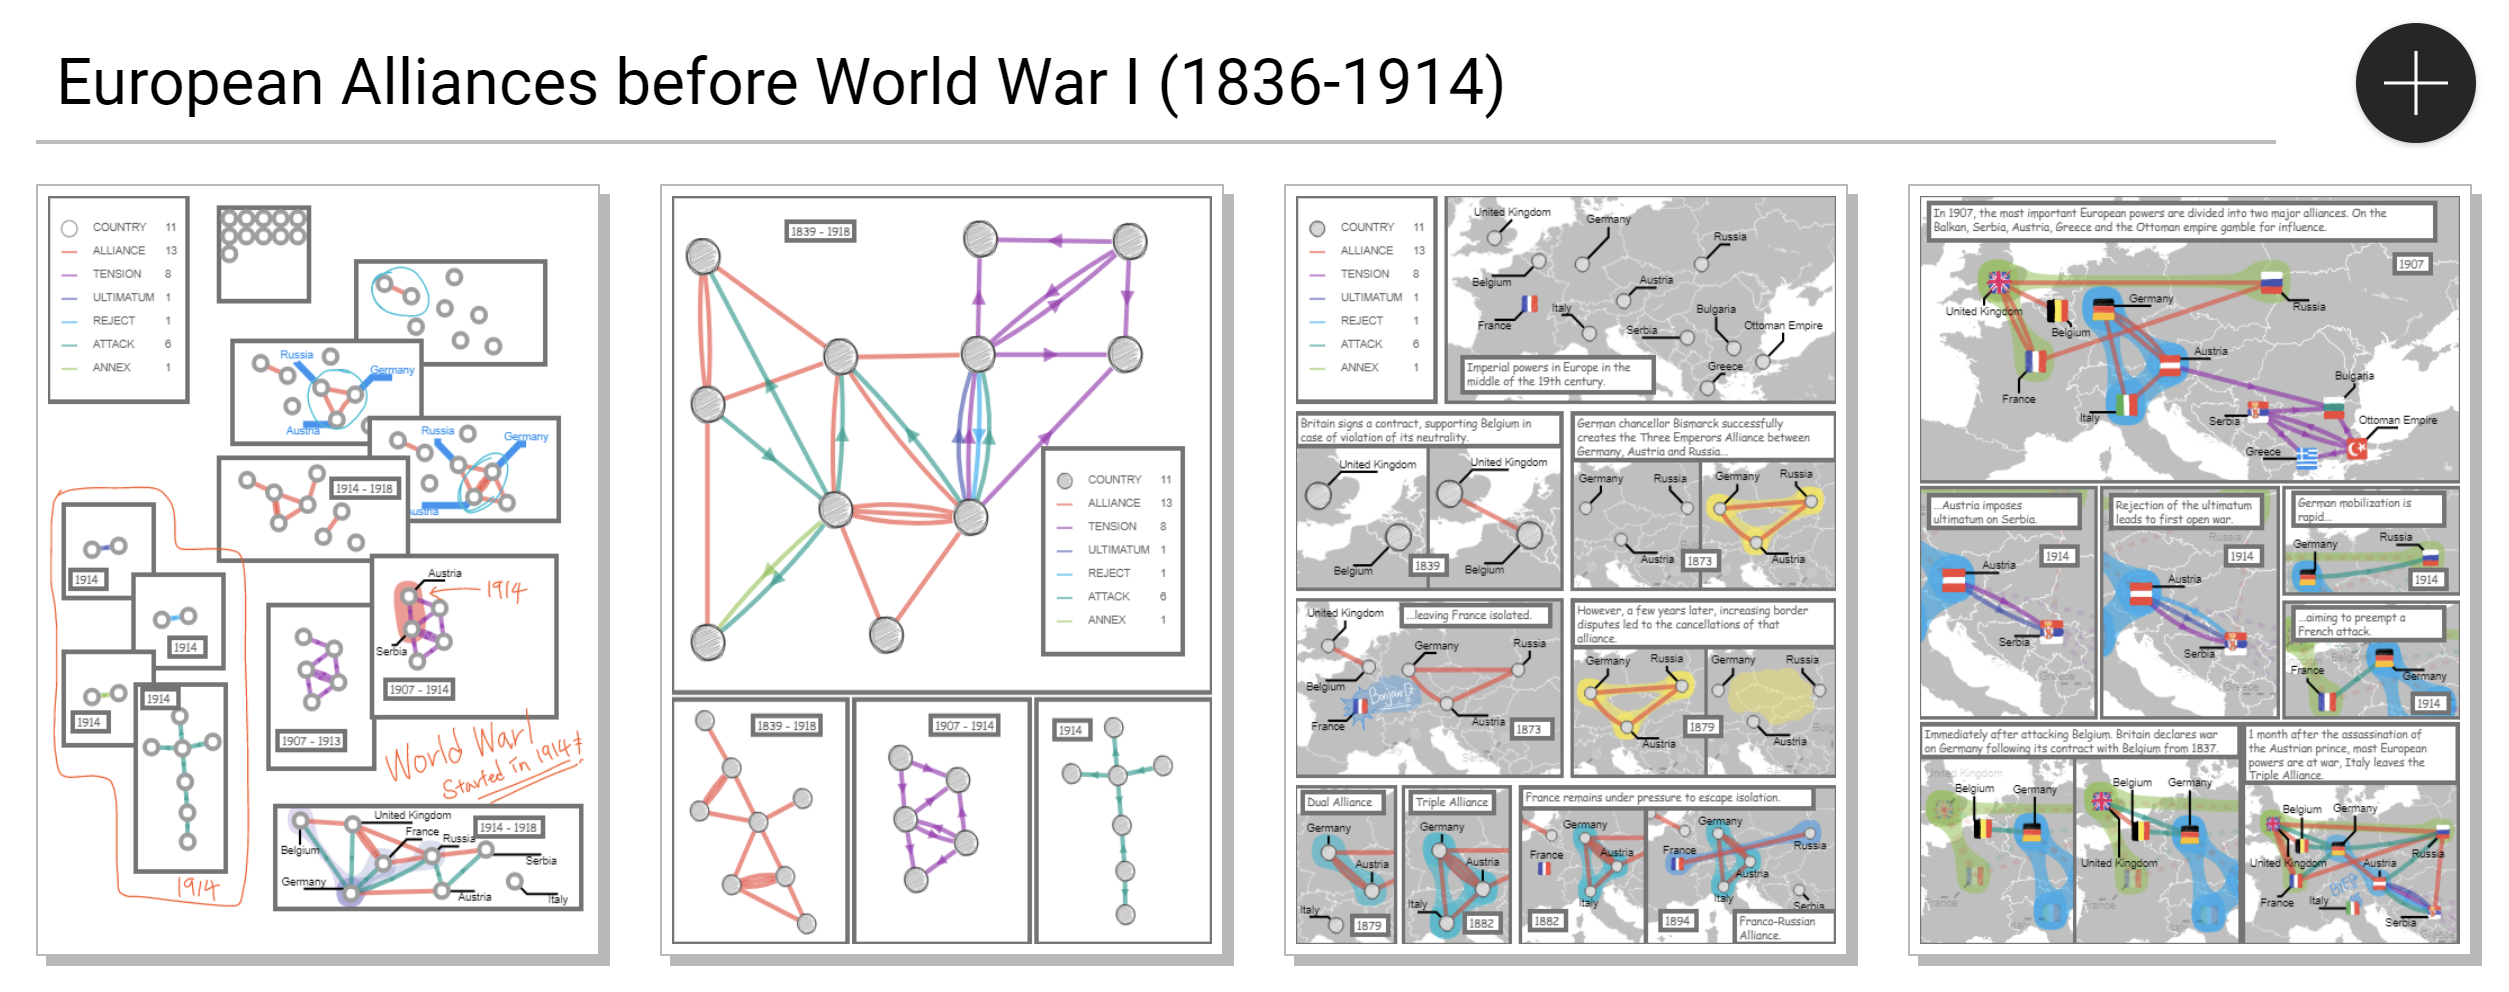
\includegraphics[width=\linewidth]{figures/comicbook} 
    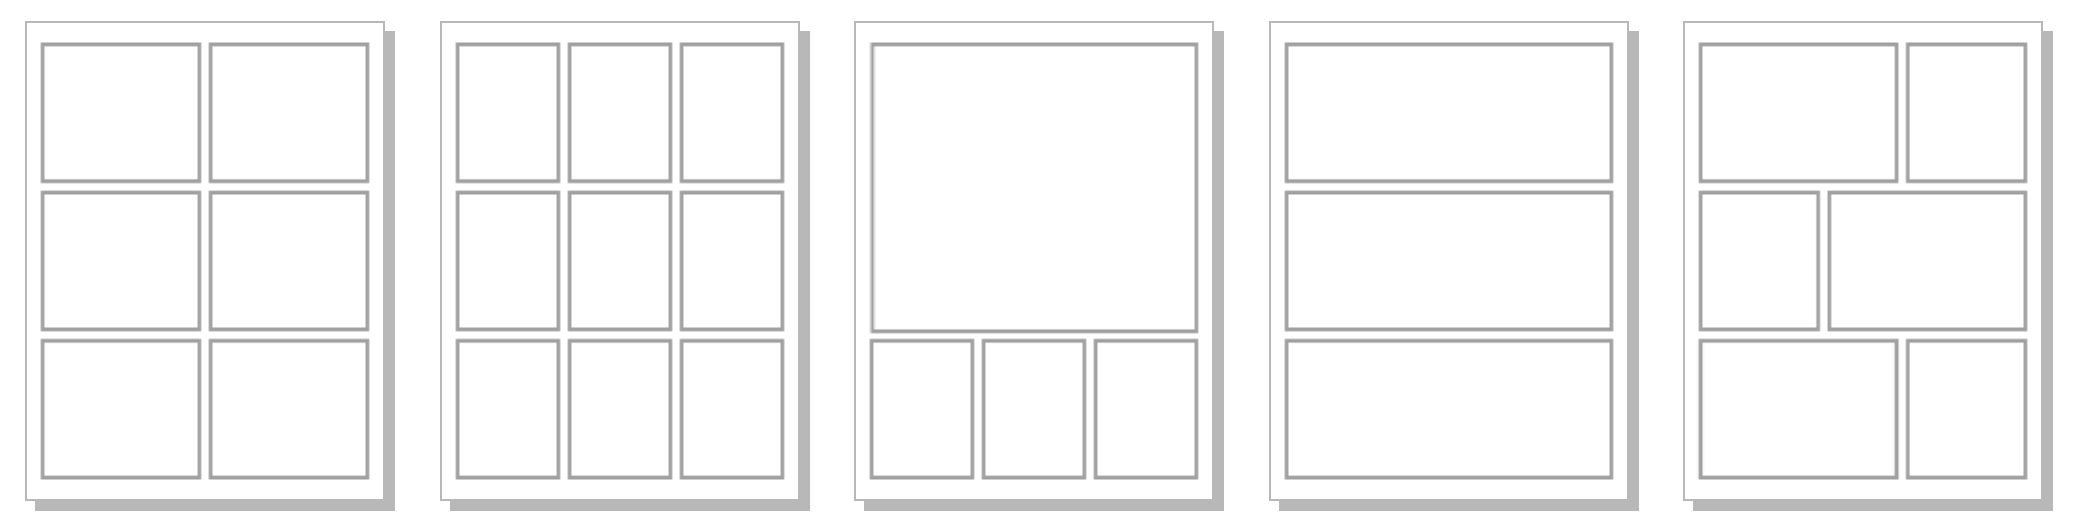
\includegraphics[width=1.0\columnwidth]{figures/layouts} 
    \caption{DataToon uses a comic book metaphor to allow authors to create multiple pages of data comics using more than one dataset. Each page can be created with a a predefined layout such as the ones shown in the second row.}
	\label{fig:comicbook}
     \vspace{-0.2cm}
\end{figure}


% Additional temporal filtering can be applied using the time slider that appears on demand when the author selects the panel (\autoref{fig:workflow}e).

% Dragging a node type onto the canvas creates a unit chart, while dragging a link type will create a node-link diagram. In a similar way, the user can progressively add more types to the existing panel to build a more complex visualization (e.g., a stacked unit chart with multiple groups of nodes and a node-link diagram with multiple groups of nodes and links). 

 

\bpstart{Acquiring different pen modes}
Content editing occurs through the use of the following pen modes:

\bstart{
\includegraphics[scale=0.03]{figures/draw_pen.png}  Pencil} mode is the default pen mode and allows for freeform inking on the canvas. If the author draws atop a content panel, the ink belongs to the panel and moves along with it when that content panel is manipulated. 

\bstart{
\includegraphics[scale=0.03]{figures/label_pen.png} Label} mode generates a text label for nodes and links and allows for adjusting label positions (\autoref{fig:teaser}F). Label and leader lines move when the element is moved.

\bstart{
\includegraphics[scale=0.03]{figures/highlight_pen.png}  Highlight} mode allows the author to lasso a set of nodes to highlight them in a colored group (\autoref{fig:teaser}F). As with labels, highlights also adjust when elements are moved.

\bstart{
\includegraphics[scale=0.03]{figures/filter_pen.png} Filter} mode allows the author to lasso a set of nodes to filter them from a panel or to create a new panel with these nodes (\autoref{fig:teaser}B). %\matt{Does one of these filter modes require pressing the pen button?}
Filtering can de-clutter panels and help focus on different subsets of the network. %\matt{violates ken's mantra}


\bstart{
\includegraphics[scale=0.03]{figures/layout_pen.png} Layout} mode leverages the high-precision of the digtial pen to adjust the positions of nodes and labels (\autoref{fig:interface}H). %\matt{also violates?} 
% The author can always resort to the automatic force-directed layout if necessary (\autoref{fig:interface}I). \matt{too much detail}

\bstart{
\includegraphics[scale=0.03]{figures/magic_pen.png} Magic} mode offers a way to automatically generate content panels (\autoref{fig:teaser}C, D), described in more detail below. 

\bstart{
\includegraphics[scale=0.03]{figures/eraser_pen.png} Eraser} mode deletes any item on the canvas including panels, ink, annotations, and highlights. This mode can also be invoked via the pen's eraser button, should it have one.  

\bstart{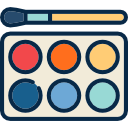
\includegraphics[scale=0.03]{figures/palette.png} Palette} mode allows the author to choose a different color, line thickness, and fill opacity, which will be applied to subsequent pencil strokes, annotations, and highlights.

% DataToon provides rich annotation and highlighting options by combining both freeform sketching and data-aware annotation (\textbf{C1}). Using the \textit{Annotation} pen, the author can lasso a set of nodes to show them in the foreground while muting the rest (\autoref{fig:workflow}f) or 

% generate a colored bubble surrounding them with the pen button pressed (\autoref{fig:workflow}h). The author can also create a node label by drawing a line out of each node (\autoref{fig:workflow}b). These types of annotations are all data-driven, making it easier to update iteratively. For instance, if the author updates the position of a node, the corresponding label and bubble are automatically updated. Just like the regular pencil, the author can choose a different style, and the selected style will then be applied to the style of the annotation. 

% \bpstart{Control 
\includegraphics[scale=0.05]{figures/control_pen.png}}
% To control which part of the content to show in the panel (e.g., cut-out or lens~\cite{bachdesign}), \toolname{} supports simple panning and zooming through the \textit{Control} pen (\autoref{fig:workflow}f). The author can also control the layout of a visualization (i.e., unit chart or node link diagram) that is initially auto-generated (\autoref{fig:workflow}b), as well as the positions of labels. 


% \bpstart{Transition 
\includegraphics[scale=0.05]{figures/transition_pen.png}}
% \toolname{} currently provides three automatic transitions, namely a temporal sequence, build-up of data dimensions, and zoom transform~\cite{bachdesign} (\autoref{fig:transitions}). To create the transitions, the author needs to draw a path from one panel to another using the \textit{Transition} pen. \toolname{} then tries to interpolate the two panels by detecting the difference between them. A typical continuous value interpolation works for the temporal sequencing and zoom transition (e.g., 2014 $\rightarrow$ \{2015,2016,2017\} $\rightarrow$ 2018). For the build-up transition, we progressively add or remove filters (i.e., node type or link type). The greater the distance between the panels is, the more transition panels are generated along the path.



% All the visual elements on the canvas can be directly manipulated through pen and multi-touch interaction. 
\vspace{2mm}
\bpstart{Drawing custom node and link representations}
% Finally,  author can update the visual encoding of the data dimension by tapping its current encoding in the legend panel .
A secondary canvas is invoked when the author taps on the iconic representation of a node or link type in the legend (\autoref{fig:interface}D). 
Within this canvas, the author can draw a new iconic representation for the selected node or link type, and this custom representation is immediately propagated across the comic for consistency (D2). 
% There are mainly two ways to modify the visual encoding, at the data point level and dimension level. When the author taps the visual encoding of a data dimension (node or link type) in the legend panel, it invokes the contextual canvas in which the author can draw a custom icon. 
The author can also invoke this canvas to change the representation of a single node or link, by tapping it with the pen while in pencil mode (
\includegraphics[scale=0.025]{figures/draw_pen.png}). 

 
%\begin{figure}[!t]
%    \centering
%    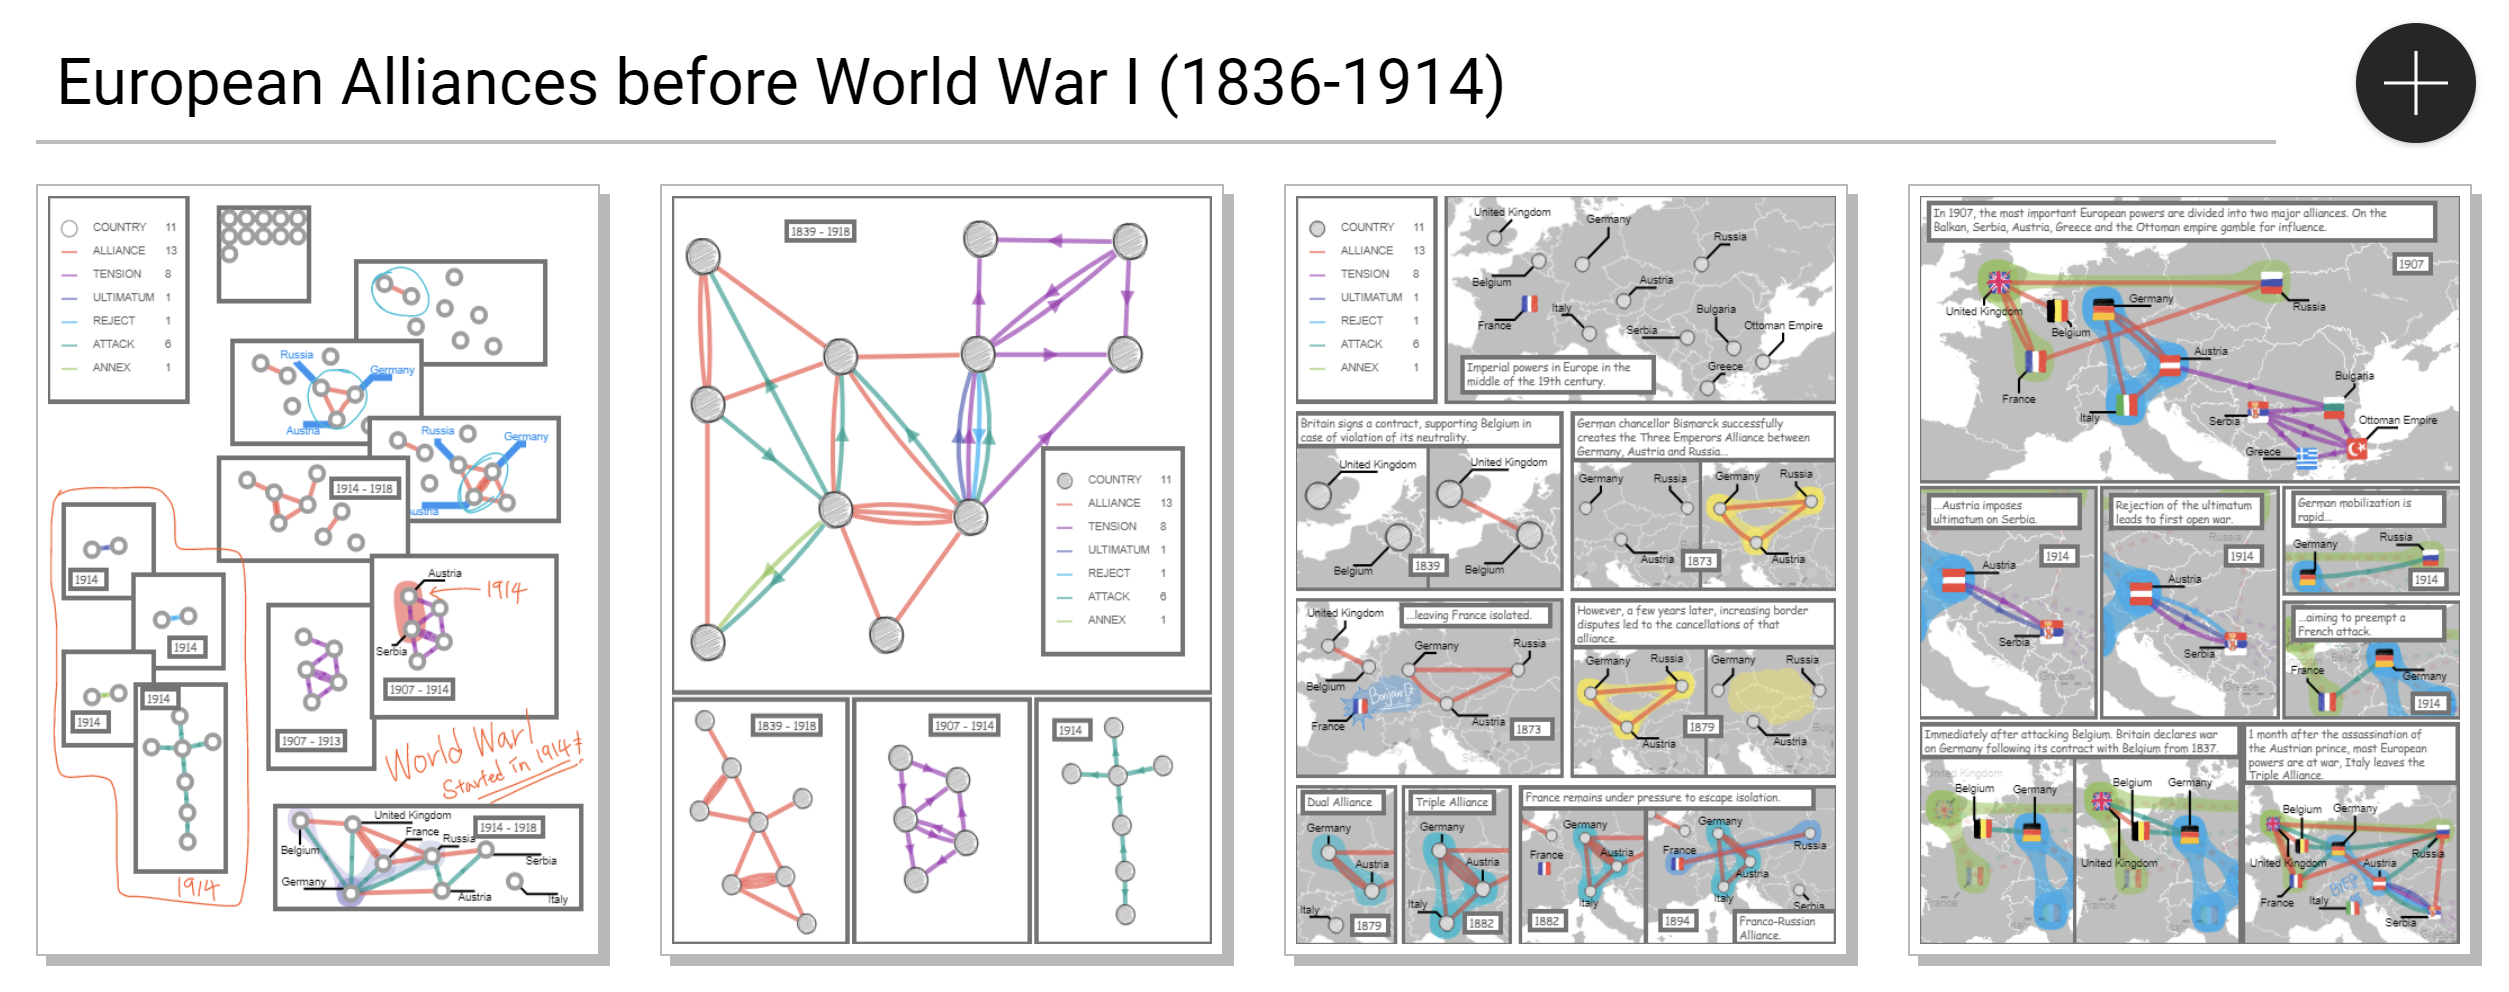
\includegraphics[width=\linewidth ]{figures/comicbook} 
%    \caption{DataToon uses a comic book metaphor to allow authors to create multiple pages of data comics using more than one dataset.}
%    \label{fig:comicbook}
%    \vspace{-0.2cm}
%\end{figure}
 
 

% \clearpage
% The reading order of the layout is assumed to follow the Z-path~\cite{cohn2014architecture}, guiding the reader from left to right, and then down). 
 

% A meaningful order and relation between a set of panels in comics can help creating a narrative [28]. A narrative can be linear, e.g., an explanation that spans over multiple panels, a sequence of question-and-answer, a temporal change, an exposé that contextualizes a dataset [11]. A narrative can further be non-linear [23, 36] or entirely open, inviting the reader to explore on their own, possibly after a guided introduction (martini-glass structure [48]). Our dimension of content relation describes how the panel content relates. Relations between just two panels have been described as transitions by McCloud [41] for traditional comics and include time steps (moment-to-moment), actions (action-to-action), characters or objects (subject-to-subject), places or scenes (scene-to-scene), aspects (aspect-to-aspect), or no specific relation at all (non-sequitur). Similar transitions have been described for data comics [10] and which reflect the more general taxonomy by Hullman et al. [33] on sequences in narrative visualizations: temporal, spatial, granular, comparison, causal, dialog. These transitions and categories have been inspirational to our dimension of content relation with some categories maintained: temporal, granular, facets.
% To alleviate the cost of generating intermediate panels

\begin{figure}[!tb]
    \centering
    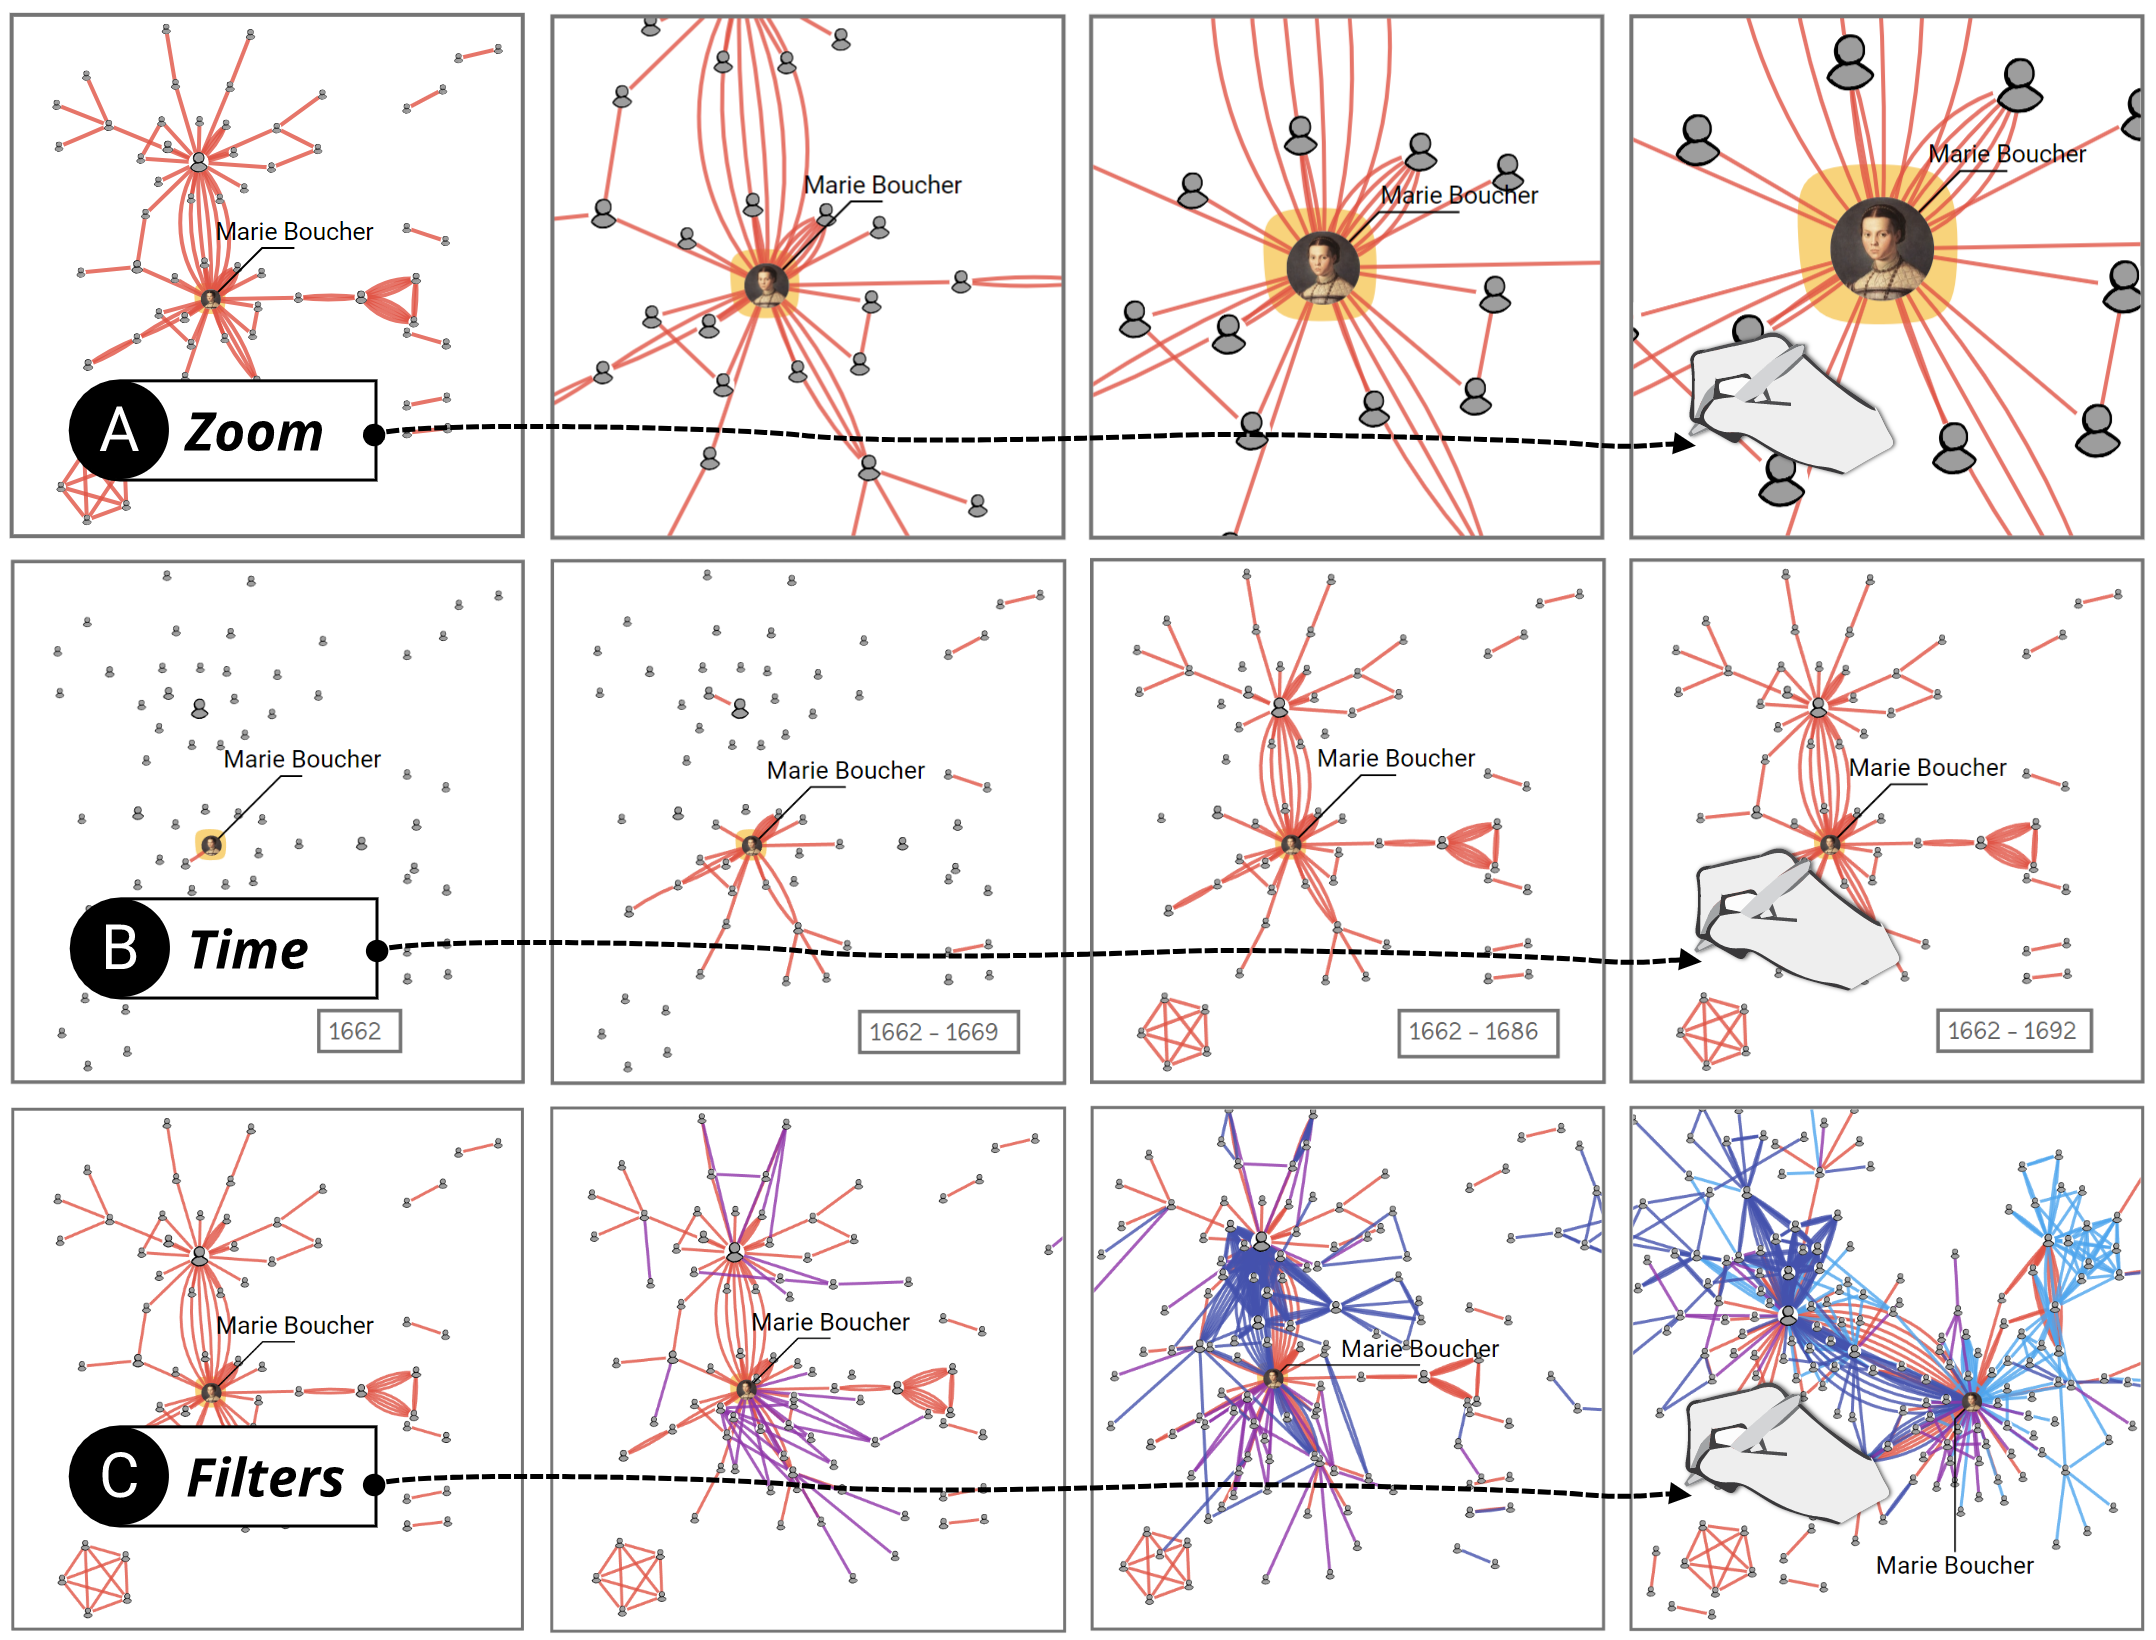
\includegraphics[width=\linewidth ]{figures/transition} 
     \vspace{-0.3cm}
    \caption{Automatic transitions between panels involve interpolating differences between panels, incorporating zoom levels, time ranges, filters, and combinations thereof.}
    \label{fig:transition}
    \vspace{-0.2cm}
\end{figure}

% \rev{geocoding if possibe}

 
 
%  as well as interactions of panel sizes. 

% Unlike a typical linear sequencing in other data storytelling tools, this can offer a nonlinear reading experience.


% panels contains a snapshot of data. scenes. time and location are 


% a visual data story consists of spatial juxtaposition of visualization panels and captions, data-driven and graphical annotations

% Panels as scenes. Each panel has data bindings determined through various filters. Pan and Zoom further defines the scene. 

% Sizing panels further allows manipulating the perception of the narrative. 
% Flow is established through the arragenment of panels. Narration is accomblished using the annotations. 

% non-linear structure
% We use space to convey both time and 

% a narrative flow
\vspace{-2mm}
\subsection{Facilitating Ideation}
\toolname{} provides several ways to scaffold and accelerate the data comics creation process (D1):

\bstart{1. Multiple pages and layout templates} facilitate the creation of multiple iterations of comics (\autoref{fig:comicbook}). Pages can load different datasets or contain different notes. Templates are a set of panel layouts commonly used in comics~\cite{bachdesign} such as grid, overview+detail, parallel, and staggered. 
When selected, the new page is auto-populated with empty content panels specified by the template. Authors can simply drag data on top of them to fill them.
% with panels based on the layout. They currently do not fill the content of the panels but are designed to scaffold a narrative structure. We leave automatically filling the content of the layout as future work. 

\bstart{2. Automatic transitions.}
% to get recommendations for next panels or between two panels to create transitions. 
\toolname{} creates intermediary panels by interpolating the difference between the two panels, taking into account their respective panel sizes, data filters, and zoom states (\autoref{fig:transition}). 
%\matt{Re: R1's review, What happens to backroung images?}
These transitions may also incorporate a temporal progression between two time filter states and the addition or removal of nodes and links~\cite{bachdesign}. 
It does not, however, attempt to interpolate annotations between two panels.

As an example, if a source panel and a target panel have zoom factors of 1.0 and 1.8 respectively, intermediary panels will have interpolated zoom factors between 1.0 and 1.8. In addition, if the source and target panels have different sizes and display data at different time periods, \toolname{} will interpolate over these dimensions as well, producing intermediary panels that would gradually increase in size and depict a progression over time intervals.  
%Similarly, \toolname{} applies a continuous value interpolation for panel size transformations and temporal sequence shifts (e.g., 1873 $\rightarrow$ [1885,1897] $\rightarrow$ 1914), progressively adding or removing nodes and links (e.g., {\textit{Alliance}, \textit{Tension}} $\rightarrow$ [ {\textit{Alliance}}, {\textit{Alliance}, \textit{Ultimatum}} ] $\rightarrow$ {\textit{Alliance}, \textit{Ultimatum}, \textit{Reject}}).

\toolname{} places intermediary panels along the path drawn by the author. Greater distances between panels results in more intermediary panels along the path. It discretizes the path and conducts a linear search for panel positions, while ensuring no overlap between intermediary panels. 

\vspace{2mm}
\bstart{3. Panel suggestions}
% To suggest next panels from one panel, it relies on detecting sub-network patterns in the panel data (\autoref{fig:suggestion}). 
 for new panels are shown in two contexts: either when loading a new dataset or when drawing a line out of a panel using the Magic pen. 
In the first case, it attempts to detect interesting subnetwork patterns in the whole dataset and places suggested panels at the left side of the canvas. 
This helps authors become familiar with the dataset and serves to kickstart the story design process. 
In the second case, it takes into account the current state of the panel and detects patterns within the panel to generate suggestions. 
It thereby enables authors to discover potential compelling directions for their story. Similar to transitions, these suggested panels are placed along the path the author draws, while preventing overlap between them. 

To detect patterns in the network data, \toolname{} relies on a pattern detection engine. The engine accepts any network data including highlighted nodes as input and returns a list of detected patterns. It currently looks for four structural patterns including articulation points (or bridges), cliques, hubs, and communities (\autoref{fig:suggestion}). Once patterns are found, it heuristically prunes the results such as by removing overlapping patterns (e.g., a bridge and a hub can often show a completely identical structure), as well as cliques with less than four nodes. Finally, it ranks the patterns based on how much each pattern overlaps with the source data. This is to promote closure between the source panel and the suggested panel. Finally, the rankings give a high priority to patterns that contain highlighted nodes (\autoref{fig:suggestion} C).

\begin{figure}[!tb]
    \centering
    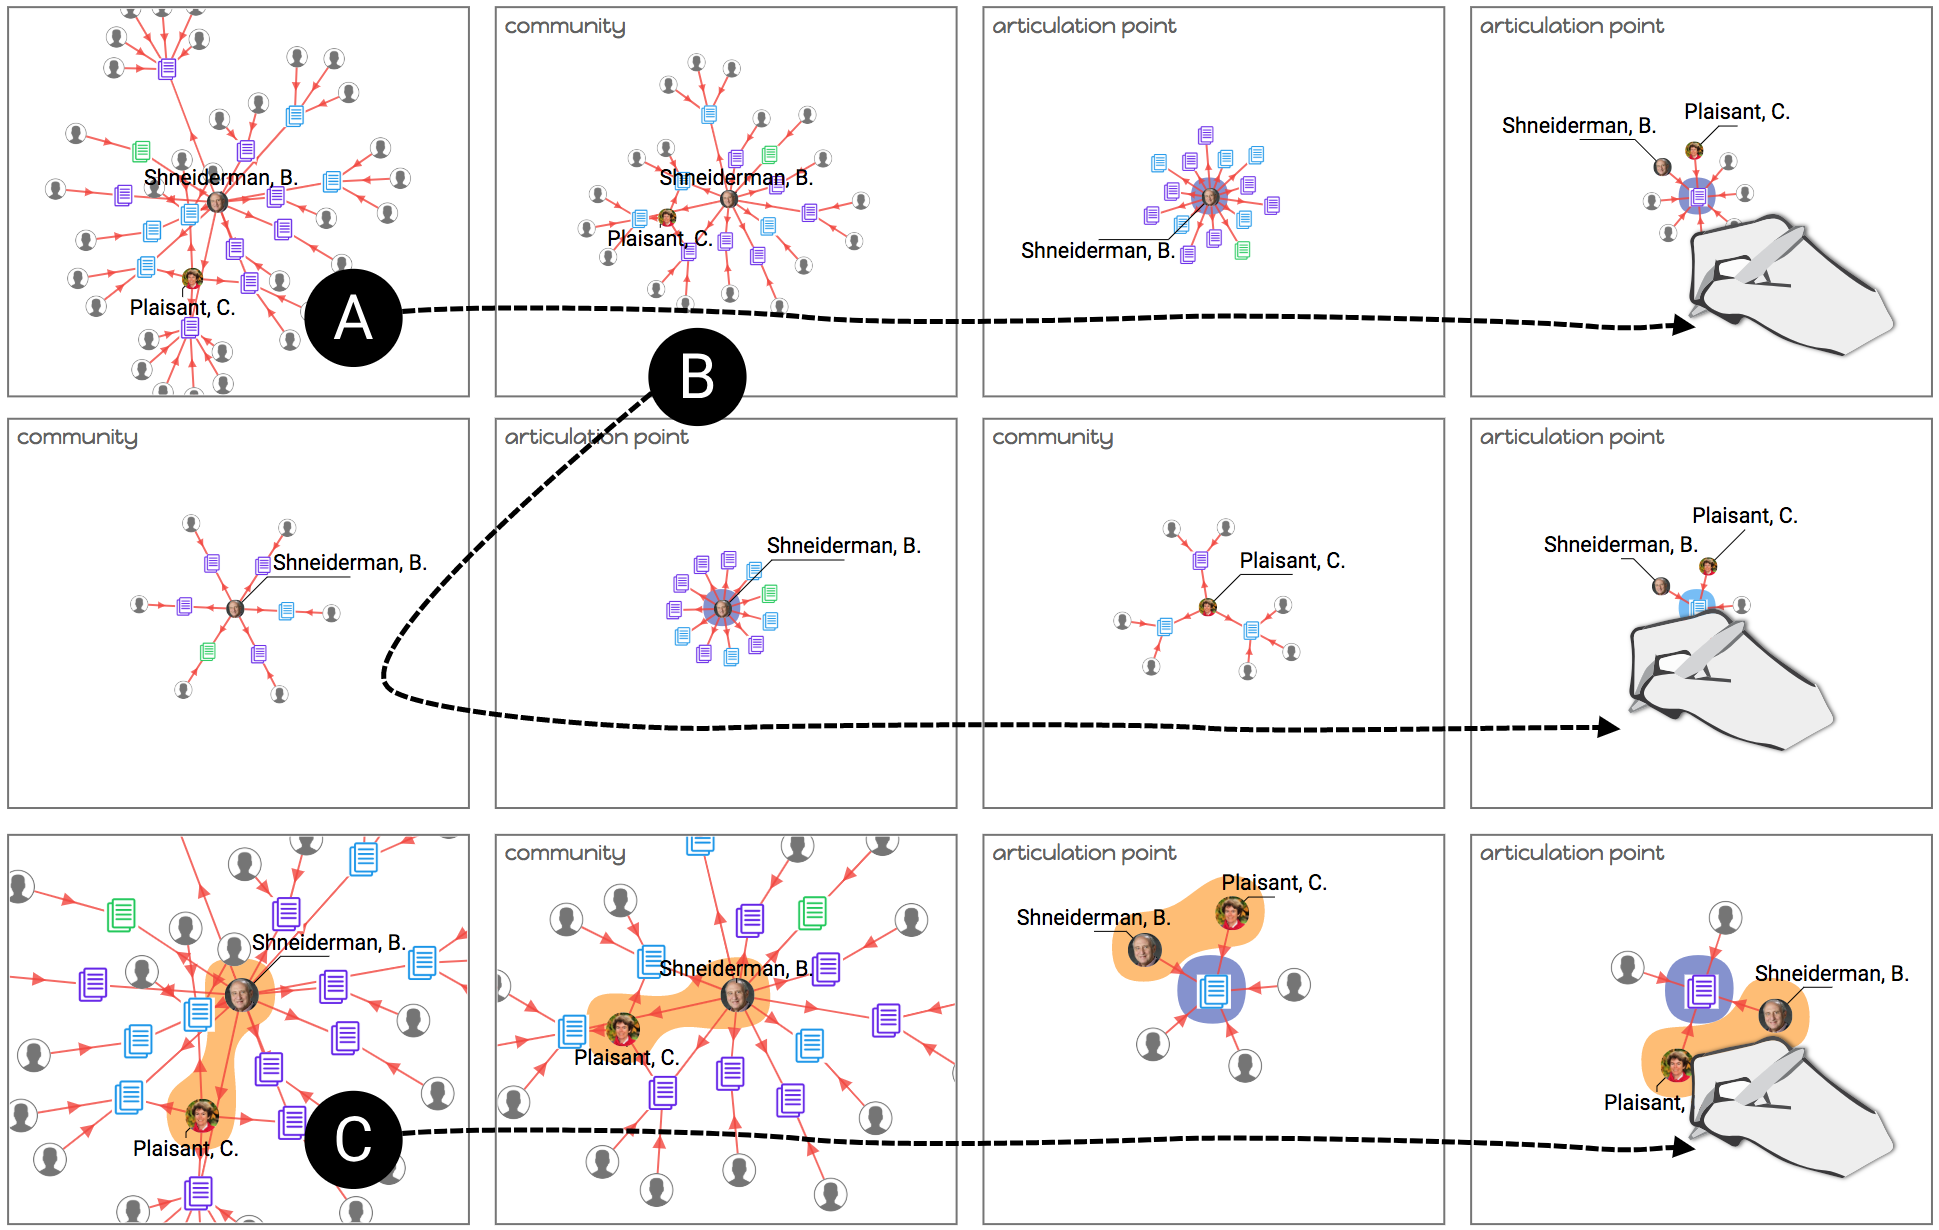
\includegraphics[width=\linewidth ]{figures/suggestion.png} 
    % \vspace{-0.3cm}
    \caption{Automatic panel suggestions depicts structural patterns: communities, hubs, articulation points, and cliques. The author can trigger suggestions from existing panels (A) and suggested panels (B). Patterns are ranked based on network coverage and inclusion of highlighted nodes (C).}
    \label{fig:suggestion}
\vspace{-0.5cm}
\end{figure}

\subsection{Implementation Details}
\toolname{} is a browser-based application written in Javascript. It uses React.js for building user interface components and Redux.js for application state management. It uses WebCoLa
~\cite{webcola} to generate the layout of the node-link diagram and a Javascript implementation~\cite{bubblesets} of Bubble Sets~\cite{collins2009bubble} to highlight a group of nodes as a cluster. \toolname{} consists of a front-end interface without a back-end server, though one can be attached if needed; currently, \toolname{} makes use of localStorage and indexedDB in HTML5 to persist the application state. The panel recommendation engine is implemented in Python and uses NetworkX to detect patterns~\cite{networkx}. 

% We also make use of utility functions in D3~\cite{d3} such as pan and zoom, and react-annotation for labelling~\cite{annotation}. 


% and available on GitHub (\rev{https://github.com/nathalieriche/datacomics/})
% 
% \begin{figure*}[!htb]
%     \centering
%     \subfigure[]{
% 	    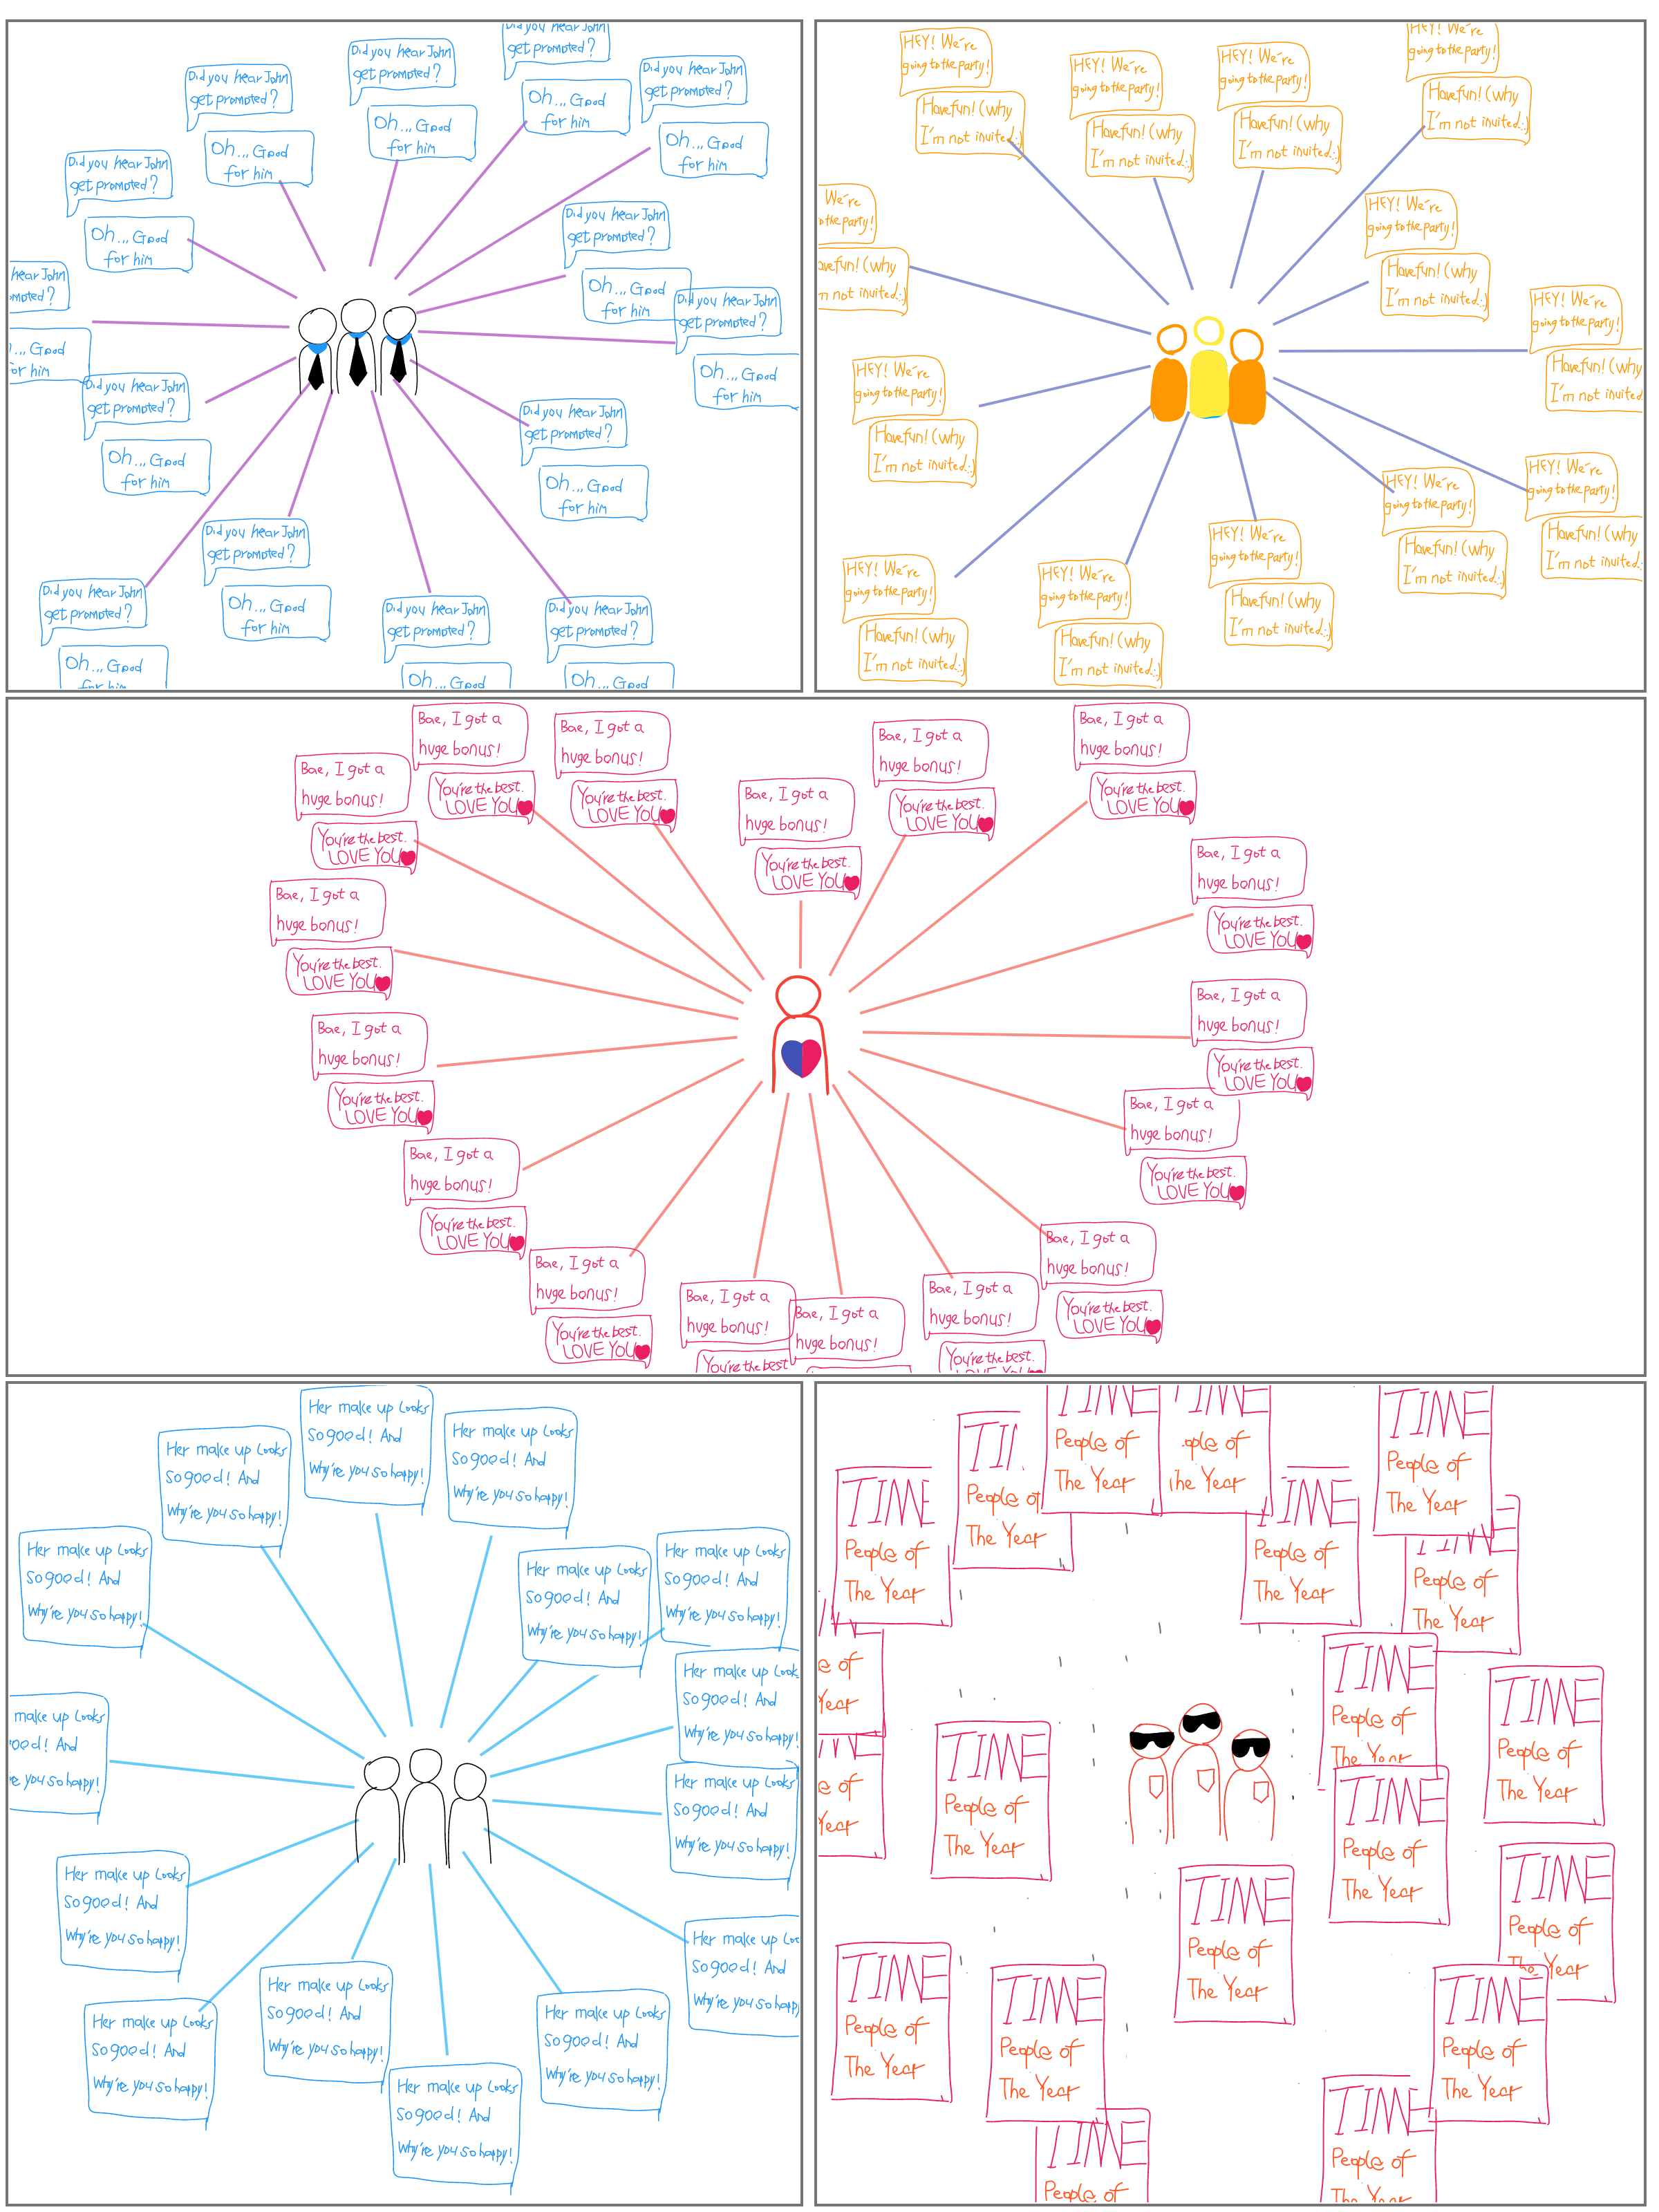
\includegraphics[width=0.25\textwidth]{figures/people}
%     }
%     \hfill{}
%     \subfigure[]{
%     	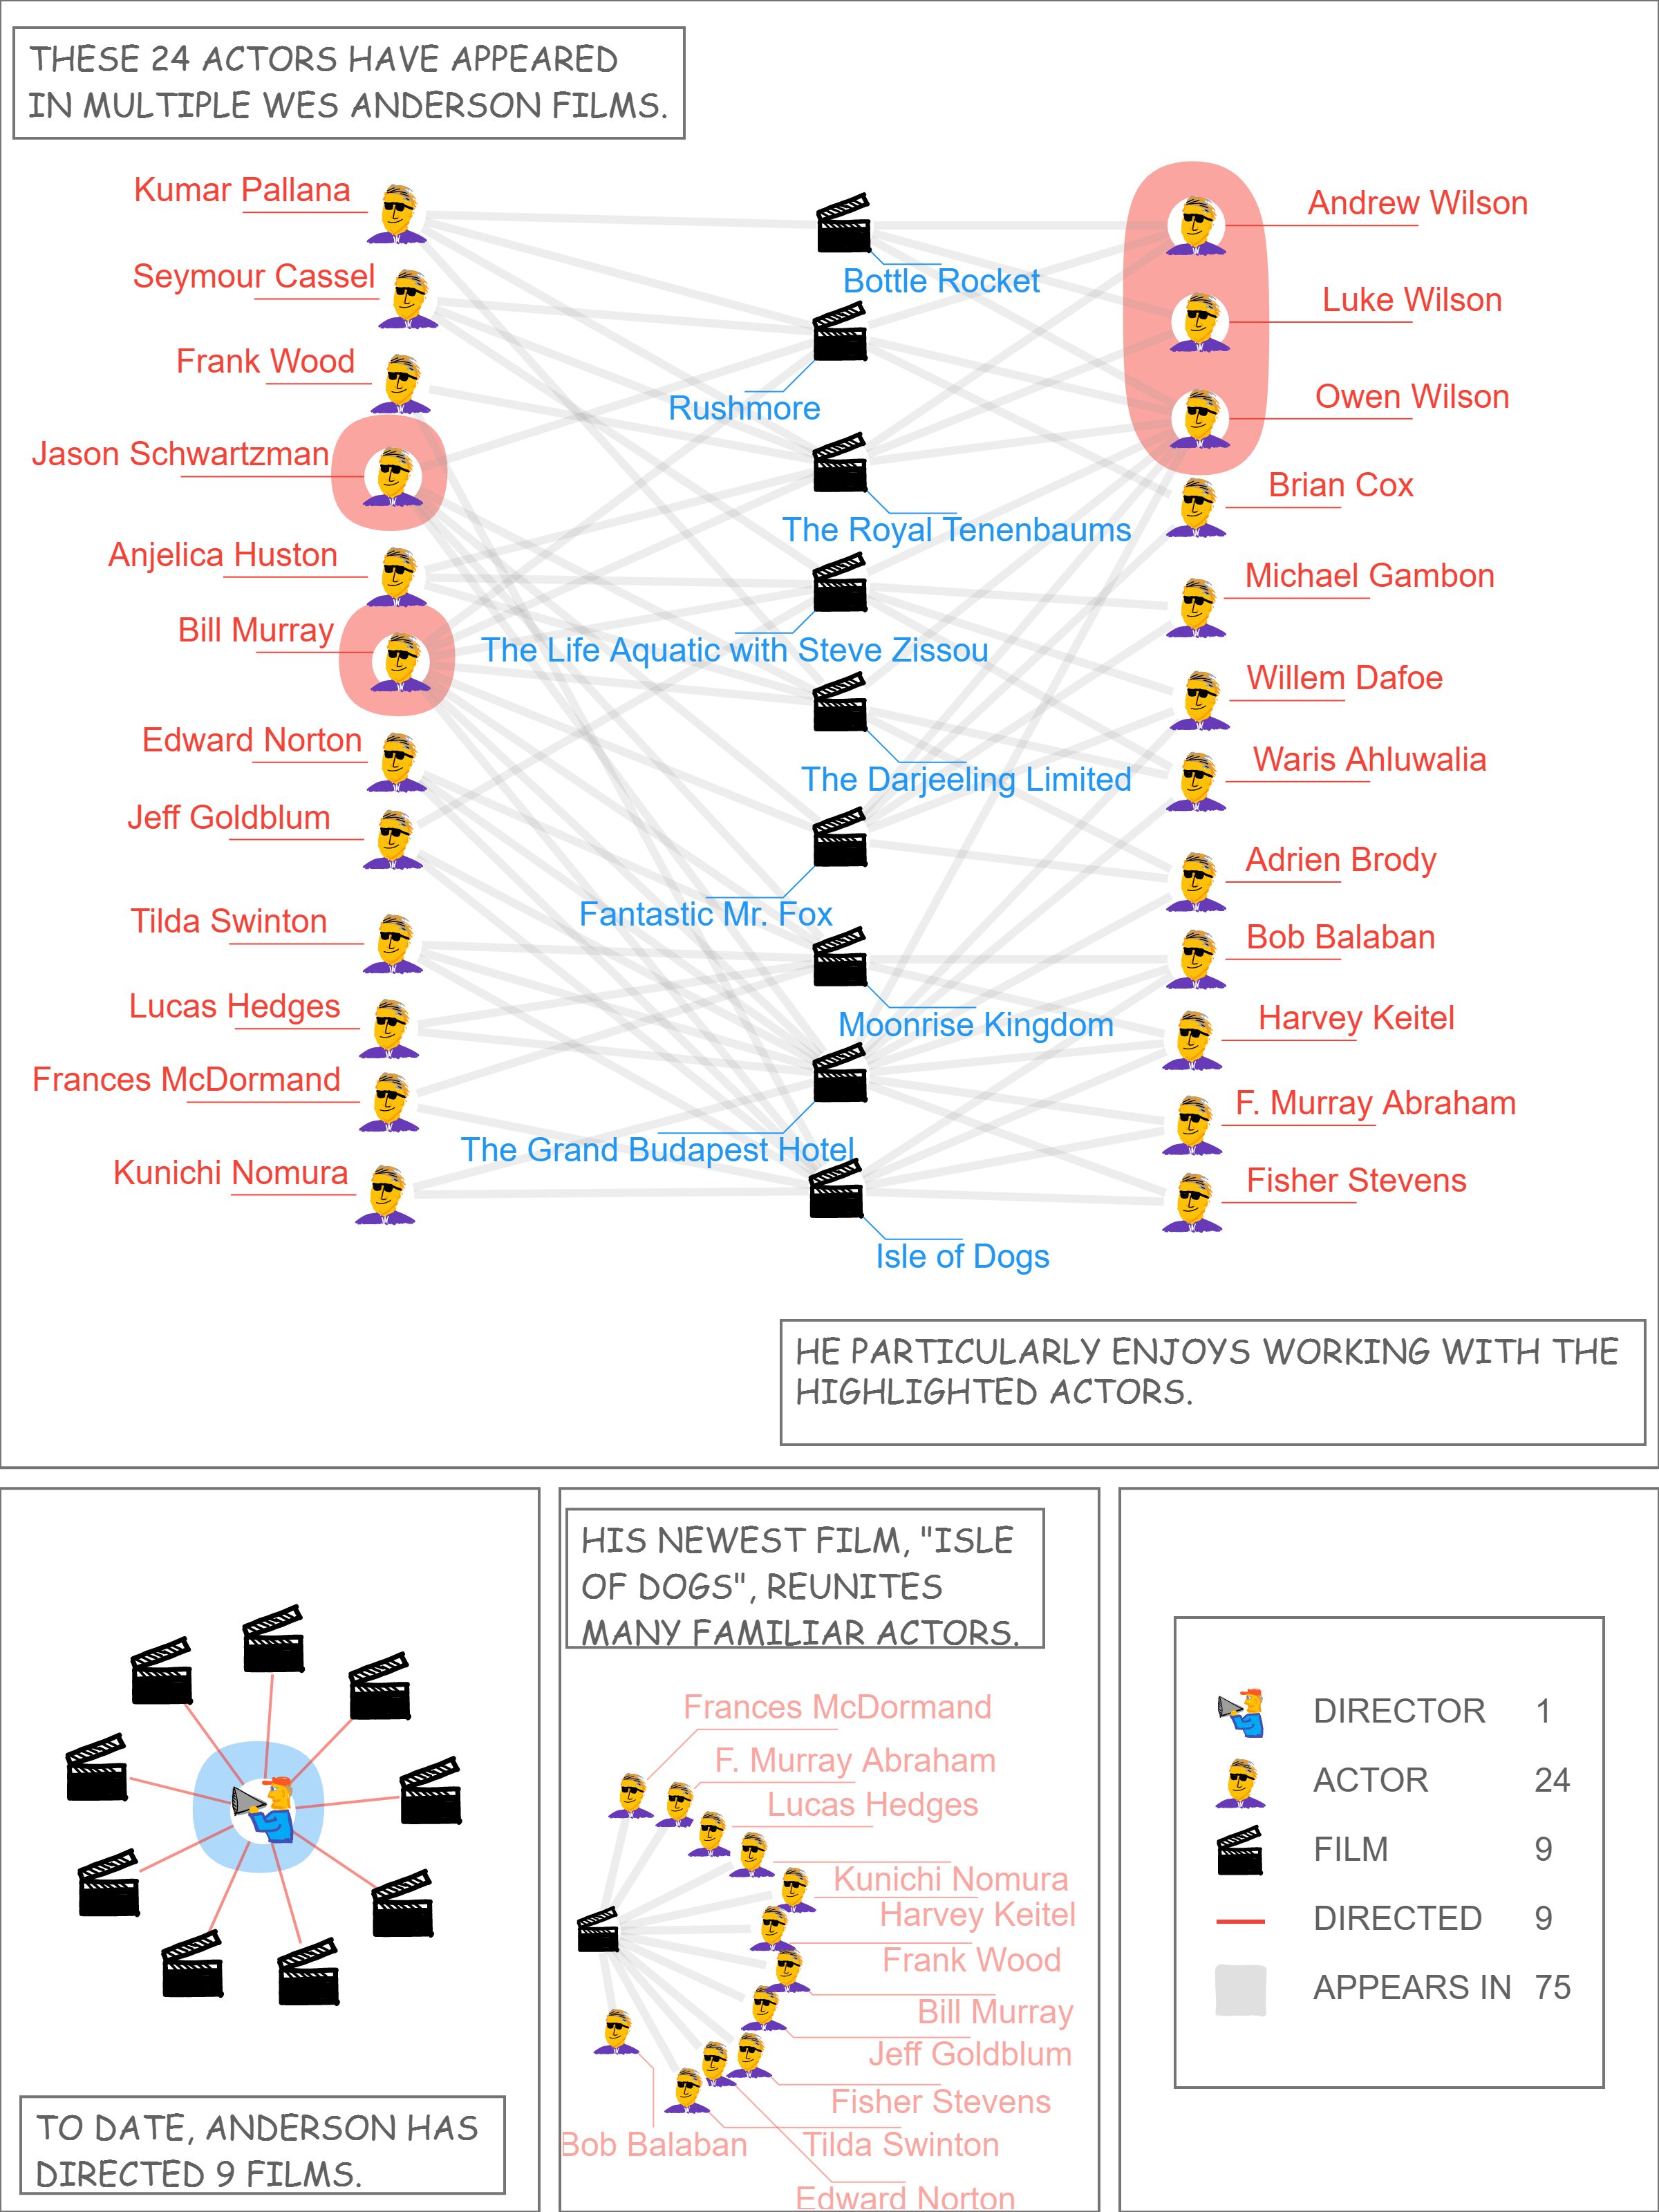
\includegraphics[width=0.25\textwidth]{figures/wes_anderson} 
%     }
%     \hfill{}
%     \subfigure[]{
% 	    \includegraphics[width=0.25\textwidth]{figures/tarantino}
% 	}
%     \hfill{}
%     \subfigure[]{
% 		\includegraphics[width=0.25\textwidth]{figures/fekete}
%     }
%     \subfigure[]{
% 		\includegraphics[width=0.25\textwidth]{figures/ben-comics}     
%     }
%     \hfill{}
%     \subfigure[]{
%   		\includegraphics[width=0.25\textwidth]{figures/marie-boucher}
%     }
% \vspace{-0.1cm}
%     \caption{Six examples of data comics created with \toolname{} using different datasets. Higher resolution versions are available in supplementary material as well as on \url{https://datatoon.datacomics.net}. }
%     \label{fig:examples}
% \end{figure*}

% \begin{figure}
%  \includegraphics[width=\columnwidth]{figures/milesdavis-2.png}
%   \caption{Data Comics created with DataToon featuring (a) expressive visuals for representing instruments (C1), (b) breakdown of pane to convey temporal evolution (C2), (c) transition between panels at different scales (C3), laid out in 2D space to convey a linear story (C4).}
%   \label{fig:miles}
% \end{figure}

% \section{Examples}

% To demonstrate the expressiveness of comics that can be created with DataToon, we assembled a gallery available in supplemental material.  Figure~\ref{fig:examples} presents six comics showing multivariate and temporal social networks and co-authorship networks, as well as networks depicting relationships around movies, actors, and directors. We refer to the specific comics in Figure~\ref{fig:examples} through letters (a-f) in this section.

% DataToon supports different styles ranging from sketchy (a,d), to clean vector-graphics (e,f), including pictures (c), as well as small pictograms for nodes (b,c,d,e). Free placement of panels allows for a variety of layouts such as described in ~\cite{bachdesign}; tiles implying a clear sequential narrative (e.g., a,b), larger panels for an overview and smaller for details (b,c). Comic (d) still employs a sequential layout but aligned in a clock-wise manner to break the convention of the zig-zag layouts. Some of the comics use sequence (panels) to show temporal evolution (d,e,f), others imply different facets (a) and details of the data (b,c). 



% \rev{or add user driven examples here?}

\section{Evaluation}

Our evaluation methodology is representative of other recent evaluations of visualization authoring systems~\cite{ren2018beliv}, in that we demonstrate the {\it expressiveness} of \toolname{} with an example gallery (\autoref{fig:examples}) and
% , where Ren~\etal~\cite{ren2018beliv} define expressiveness as the scope of possible visualization design choices enabled by a system. 
also evaluate its {\it learnability} and {\it usability} via a reproduction study.

\subsection{Example Gallery}
% \nam{do we need to say this: While we did not formally evaluate the range and expressivity of data comics created with \toolname{}, several co-authors, co-workers, and participants of the study used it to create comics; \autoref{fig:examples} showcases some of these.} 
\rev{\autoref{fig:examples} shows example comics varying in their comic style, including diverse rendering styles (abstract, sketchy, realistic), panel layouts (inset, overlapping, staggered)~\cite{bachdesign}, visualizations (unit charts or pictographs, maps, set visualizations, node-link diagram), and narrative structures (overview+detail, nonlinear-temporal, cut-out, build-up~\cite{bachdesign}). The gallery also exemplifies a diversity of datasets, including multivariate and temporal social networks and co-authorship networks.}

% \deleted{The examples encompass a diversity of datasets, including multivariate and temporal social networks and co-authorship networks, as well as a variety of comic styles, ranging from sketchy to precise.} The gallery also exemplifies different narrative patterns~\cite{bach2018napa} showing temporal evolution or iteration over different dimensions of the data. 
%We also included videos of the authoring processes for these examples in our supplemental material.
%~\rev{can we?} \matt{As videos?}.
 
\subsection{Reproduction Study}
%\matt{This paragraph addresses R4's comments, who focused way too much on the study}
To evaluate whether people can learn how to use \toolname{} to create comics from data, we conducted a qualitative reproduction study, in which participants are asked to reproduce them completed examples with \toolname{}. 
This type of study is particularly common in the evaluation of visualization authoring tools~\cite{ren2018beliv}, having been used to evaluate Lyra~\cite{satyanarayan2014lyra}, ChartAccent~\cite{ren2017chartaccent}, DataInk~\cite{xia2018dataink}, Data-Driven Guides~\cite{kim2017data}, Data Illustrator~\cite{liu2018data}, and Charticulator~\cite{ren2018chart}. 

\vspace{2mm}
\bpstart{Participants} 
We recruited eight participants from a large software company in the United States. Half of the participants were graphic designers with limited data literacy (P1-P4: 3M, 1F; ages 30$\--$50, avg: 44), while the other half were data analysts with minimal experience in design tools (P5-P8: 2M, 2F; ages 31$\--$42, avg: 37). 

\vspace{2mm}
\bpstart{Apparatus}
Participants used a earlier version of \toolname{} on a Microsoft Surface Studio with a 28-inch screen at 4500 $\times$ 3000px (192 PPI), a device that enables simultaneous pen and multi-touch input.

% From the graphic designers we sought to gather feedback on the interface paradigms we selected and implemented in \toolname{}, to assess if key interactions or concepts were missing to produce data comics, and to gain an understanding of how it compares with tools that are more oriented to graphic design. From the data analysis, we aimed to assess whether they can learn \toolname{} and use it to create comics from data without guidance.  

%\bstart{Participants}
% We recruited our eight participants from a large software company in the United States. The graphic designers (P1-P4: 3 males, 1 female, aged 30 to 50, average 44) had professional experience in graphic design (e.g. over 20 years of experience using Adobe Illustator). Three of them had relatively low expertise in data analysis but one reported creating charts from data on a monthly basis. The data analysts (P5-P8: 2 males, 2 females, aged 31 to 42, average 37) perform data analysis and create charts and visualizations as part of their job. They had low or no experience with graphic design tools. All participants received \$20 in lunch coupons for their time. Three of our participants were left-handed.

%\bstart{Apparatus}
% We used a Microsoft Surface Studio with a 28 inch screen at 4500$\times$3000px (192 PPI) enabling simultaneous pen and multi-touch input.

\vspace{2mm}
\bpstart{Procedure and tasks}
Beginning with a demographic survey, each study session lasted $\sim$90 minutes, with two participants finishing in $\sim$60 minutes, and one taking $\sim$120 minutes. \rev{We asked them to reproduce two comics: 1) the first with guidance from us using the comic about \textit{World War I alliances} (\autoref{fig:interface}) and 2) the second without any assistance using the comic inspired by Fathom's {\it Scaled in Miles} project~\cite{fathom} about the evolving instrumentation on Miles Davis' records (\autoref{fig:examples}-left).
The first task served as a training session and lasted 30 to 40 minutes, which included a 15-minute tutorial, while the second task lasted between 30 and 50 minutes.} The study ended with three Likert-style questions about ease of use \& learning, and enjoyment, along with a semi-structured interview about their experience.
%using \toolname{}.

% In the beginning, the experimenter asked each participant to complete a demographics questionnaire, then asked them to create two data comics (\#1,\#2) with \toolname{} and concluded with three 7-point Likert scale questions (ease of learning, ease of use and enjoyment) as well as a short interview. %\ben{on the tool, I guess?}
% \bpstart{Comic \#1: Demonstration and exploration} 
% In this first task, we asked participants to reproduce the data comic from our usage scenario about \textit{World War I alliances} (\autoref{fig:interface}), which we provided as a printout. We encouraged participants to experiment with \toolname{} until they felt comfortable to proceed without additional guidance from us. This task served as a training session and lasted 30 to 40 minutes, which included a 15-minute tutorial.
% about the capabilities of \toolname{}.


% With the first comic, participants had to replicate a data comic on \textit{World War I alliances} depicted in \autoref{fig:tool_overview} and provided as a print out.  This phase served as a tutorial and training for participants to learn and explore what was possible with \toolname{}. The experimenter presented the main principles of the interface and demonstrated the interactions required to create comics. At the end of this tutorial, participants started from a blank page and proceeded to recreate the comic, asking questions as needed. Participants were encouraged to try their own experiments with the tool until they felt comfortable to proceed without guidance. This first task lasted 30 to 40 min (including the 15 min tutorial).

% \bstart{Comic \#2: Replication without guidance}
% In the second task, without any guidance from us, we asked participants to reproduce a data comic inspired by Fathom's {\it Scaled in Miles} project~\cite{fathom} about the evolving instrumentation on Miles Davis' records (\autoref{fig:examples}-left); as with the first task, we provided the completed comic as a printout. We asked participants to think aloud as they worked, and we proceeded to observe and note usability issues, participants' utterances, commonly used features, as well as features that were left unused. This task lasted between 30 and 50 minutes.

% This time, the experimenter did not offer any guidance. 

\subsection{Observations}
All participants successfully completed both comics, while we discovered several usability insights into the usability of \toolname{}. We describe our observations below.

% P2 required a few hints to recall how to achieve some design elements in the second task.
% Based on the Likert responses, participants found \toolname{} to be easy to learn and use and they enjoyed using it.
% at 5.6/7 for ease of learning, 5.9/7 for ease of use, and 6.5/7 for enjoyment.

% Seven participants used \toolname{} without any guidance from the experimenter to replicate the second comic. 

% One participant required a few hints to recall how to complete certain interactions. On average, participants rated \toolname{} at 5.6 out of 7 for ease of learning and 5.9 out of 7 for ease of use. %\ben{What about 'enjoyment'?} We now discuss additional findings. 


%problem with conflicting interaction paradigm of the OS - pen as stylus
%P7 wanted to use pen as a stylus (right after draggging from folder)

\vspace{2mm}
\bpstart{Learning to interact with both pen and touch}
All of the participants appeared to grasp \toolname{}'s interaction design by the end of the study, except for P2, who had no prior experience with pen + touch devices. It took a long time (approx. 10 min) for P2 to complete the first task and the effort spent to learn the interactions are reflected in their low ease of learning (3/7) and use (4/7) scores. P4, P5, P6, and P7 also repeatedly appeared to be frustrated when attempting to use pen and finger interchangeably, with P7 stating \textit{``I kept using my hand instead of the pen''}.

% Other participants made minor comments 

Participants bimanual pen and touch interaction to be engaging, with P8 remarking on the simplicity of the interactions: \textit{``I love the power of just dragging} [shows fingers] \textit{and creating} [shows the pen]\textit{''}. P4 spoke about the empowering experience of bimanual pen and touch input for content creation, making \toolname{} \textit{``unique''} and \textit{``fun''} compared to other tools: \textit{``I feel like a surgeon because I got precise and used both of my hands, not something I do ever. It's pretty cool!''}.
% While not complained, we also observed several other participants (P4, P5, P6, P7) repeatedly had issues by trying to use pen and finger interchangeably. 

% During the first task, We also observed that several other participants  repeatedly having issues with bimanual interaction.

% Their additional learning effort was reflected in the time to complete the first task (10 minutes longer than other participants) and the final ratings, 2 to 3 points lower than other participants for ease of learning (3/7) and ease of use (4/7). 

% During the first task, the experimenter also observed four other participants (P4, P5, P6, P7) repeatedly having issues mastering bi-manual interaction. The main issue faced by all participants was the desire to use pen and finger interchangeably.  However, only P2 and P6 reported it as a significant usability issue in the interview: \textit{``I kept using my hand instead of the pen''}.

% From the other six participants, we received many comments on the benefits and the engaging nature of bi-manual pen and touch interaction, once mastered. This is also reflected in the final ratings as the average enjoyment of using our tool is over 6 out of 7. 

% P8 commented on the simplicity of the interactions: \textit{``I love the power of just dragging} [shows fingers] \textit{and creating} [shows the pen]\textit{''}. P4 commented on the empowering experience it provided, making the app \textit{``unique''} and \textit{``fun''} compared to other tools: \textit{``I feel like a surgeon because I got precise and used both of my hands, not something I do ever. It's pretty cool!''}.

\vspace{2mm}
\bpstart{A focused tool set for design exploration}
The graphic design participants all expressed that one notable strength of \toolname{} was a \textit{``focused tool set''} (P1), its interface \textit{``streamlining the set of tools''} (P4) compared to existing illustration tools. We observed that our interface enabled alternative workflows to achieve the same result, reflecting what Ren~\etal~ refer to as the {\it flexibility} of a visualization authoring tool~\cite{ren2018beliv}. For example, several participants began with multiple panels, adjusted the content of each panel before customizing each of them in turn. Others would create and modify one panel until it was polished, only then duplicating to instantiate the next panel.

% Three of our graphic designers also commented that the look and feel of the interface, \textit{``the soul of the app, this handwritten feel''} (P1), and sketching on a canvas were features that encouraged them to explore, ideate, and generally experiment with different data comic designs.

% For example, all but one participant replicated the first comic using a different order of interactions than demonstrated by the experimenter. We also observed a large variation in working styles between participants. Design explorations also varied from participants: some created many panels, altering and erasing them and recreating new ones to iterate while other participants worked mostly in a single panel, extensively using the undo/redo feature. 

% One particular challenge for those using these types of authoring interfaces (having a focused set of instruments with different functions, as opposed to an exhaustive set of menus and buttons) is that it may prove intimidating upon first use, since many functions are hidden. This was particularly true for our data analysts. \textit{``Minimalism is in, it looks just like a simple drawing app, but then it can be intimidating because how do you achieve all of this?} [pointing to print out of the data comics] \textit{I was nervous''} (P8). However, it is worth noting that all participants mastered the interface after the first task.

Participants' difficulties often related to feature discoverability, as not every pen mode was visually shown in the interface. For example, in the version of \toolname{} used in the study, the pen button was used to activate the highlight pen. P8 commented that \textit{``Minimalism is in, it looks just like a simple drawing app, but then it can be intimidating because how do you achieve all of this?} [pointing to print out of the data comics] \textit{I was nervous''}. Similarly, P1 commented that the principle of dragging and dropping elements into panels was violated in the case of time captions, which required a double tap, making it challenging to discover. 



% small inconsistencies in interaction principles can rapidly degrade the experience and make it hard for participants to remember how to perform specific operations.

% For example, P3 noted that an inconsistency where holding the pen button selected items when in pencil mode but it inked when used as a highlighter, which caused him to repeatedly make errors in the tutorial. P1 also commented that the general principle of dragging and dropping elements into panels was violated in the case of time captions, which required a double tap, which made it particularly challenging to remember. 



%P5  also expressed doubts on remembering \textit{"the huge number of interactions"} but commented that he remembered more than he originally thought.


%Another challenge, for our data analysts (P5-P8), who were unfamiliar with graphic design and sketching apps, is that 
%on remembering the \textit{"right order of instructions"}, taking a deep breath and stating ~\textit{"Now that's the hard part [make the largest illustration of Miles Davis albums]"} but then he proceeded to complete the panel in less than ten minutes and expressed surprised and proudness of his illustration. 

%- P1 and P4 noted the "focused toolset" (P1) streamlining the set of tools to learn and use for a specific task. 
%- P1 on time label generation (double tap inconsistent from other gesture) "if your remember that, that is really cool"
%- graphic designer P3 pointed out inconsistency in holding button to ink instead of select in annotation mode

%-P8 "When I looked at this [print out of comics], I thought it would be difficult but it is not as I thought it would be"
%- minimalism (just different instruments) but for non experts it could be intimidating


%- p3: like the richness in expressiveness, more freedom than with other tools, sketchy prototyping feel. lots of potential in this vein. 
%- P1 on captions "I feel like this one I want to handwrite it" -> turn font into sketchy. P1 "This is kind of the soul of the app: getting this handwritten feel"
%- P6 "Now, I'm going creative" "When I said I was no artist, that's it" "Oh it does not look that bad"



\vspace{2mm}
\bpstart{Closing the gap between analysis and storytelling}
Participants appreciated the ability to discover patterns during the story authoring process, suggestive of a possible advantage over visualization authoring tools that are disjoint from data analysis tools. We observed that data analysts tended to explore the data before constructing on their comics. For example, P5 started by creating many panels (one per node type) and by commenting on the structural patterns in the data. P8 used a different strategy, adding each node type to a single panel in succession, where each node type was a different instruments featured on Miles Davis records; upon doing so, P8 stated that \textit{``now I am beginning to see the relationships between instruments [...] I am going to move things around so I can understand my data''}. Finally, some participants noted the necessity of additional data abstraction. For example, P3, looking at a particularly dense node-link diagram, said \textit{``I wish there were a way to untangle that because that is a super full graph''}, suggestive of a need for capabilities that aggregate nodes and links.
\vspace{-0.2cm}


%- P8 "I am scared to erase" (thought she would loose her data)

% Data analysts (P5-P8) particularly enjoyed using \toolname{} (rated enjoyment as 6.5/7 on average), many commenting that they were not artists or did not know how to draw but yet made aesthetically pleasing visuals: \textit{``the appearance of the cartoons was much nicer than I could have created''} (P7). P8 also noted that she liked \textit{``being shielded from all the data complexity and just focus on presentation''}.
%- p7 "When can I have it"

%- for data analysts feels like they can focus on presentation (shield them from data complexity)
% As participants created comics, we gathered a number of comments on the possibility to transform visual representations of data into more ``designed'' illustrations to make insights more salient. 

% For example, P3, looking at a particularly densely connected node-link diagram, commented \textit{``I wish there was a way to untangle that because that is a super full graph''} and asked if we had features (such as bundling or link aggregation) to simplify the visualization in places to illustrate that two of its clusters were highly connected. P3 then reflected that \textit{``there is an interesting balance between what I want to provide you with a sketch to give you a general idea of the data but not show ALL the data''}.  We believe that supporting this subtle shift from data visualization towards what we call \textit{information design} is an interesting direction for future work.
\vspace{2mm}

\subsection{Lessons Learned from the Reproduction Study}

\rev{The results of the study illuminated a set of usability insights regarding the difficulty of discovering features, the inconsistency of pen and touch interactions, and the complexity of visualization contents. These insights led to several improvements to the design of \toolname{}.}

\rev{To address the feature discoverability issue, we ensured that all pen modes are visible (\autoref{fig:interface}A) without cluttering the interface and degrading the authoring experience. In addition, after observing participants repeatably attempting to use fingers where we enforced use of the pen, which initially included panning and zooming panel content, we opted to accommodate more touch interaction, reflecting \textit{the pen writes, touch manipulates} mantra~\cite{hinckley2010pen}. We also replaced the double-tap gesture for creating time captions with a consistent drag gesture. Finally, to handle the visual complexity issue, we added the ability to filter nodes of interest from a panel, as well as the panel suggestion functionality for assisting with exploring complex data.}






% Based on the observations and feedback from the reproduction study, we made several improvements to \toolname{}. The previous version of \toolname{} used in the reproduction study is available as supplemental material for comparison. %\matt{release process for a website will not be done in time for a CHI submission} 
% First, after observing participants repeatably attempting to use fingers where we enforced use of the pen, which initially included panning and zooming panel content, we opted to accommodate more touch interaction, reflecting \textit{the pen writes, touch manipulates} mantra~\cite{hinckley2010pen}. To address the feature discoverability issue, we ensured that all pen modes are now visible (\autoref{fig:interface}A), without cluttering the interface and degrading the authoring experience. We also replaced the double-tap gesture for creating time captions with a consistent drag gesture. We also added the ability to filter nodes of interest from a panel. Finally, we added the panel suggestion functionality for facilitating rapid and iterative storyboarding (C4). 

% \rev{add deployment in the wild and user driven examples}



% - phase 1 participants used tools in different orders than demonstrated.
% - participants with no data expertise required more explanation about data.  
% - from graphic design participants, we solved a few bugs and added the following features to the tool: lock, undo, sketchy font
% - three left-handed participants  (PXXX) suffered a bit from the zoom slider
% - participant who had no previous pen and touch experience (P2, others?) struggled with bimanual interaction
% - participants all co-adapted to zoom interaction although X of them started repeatedly using pinch and zoom in panel

% graphics:

% Easy to learn: 1 (p1), 5 (p2), 3 (p3), 2 (p4),       2 (p5), 1 (p6), 2 (p7), 3 (p8)
% Easy to use: 2 (p1), 4 (P2), 2 (p3), 1 (p4),         2 (p5), 3 (p6), 1 (p7), 2 (p8)
% Enjoyment: 1 (p1), 3 (P2), 3 (p3), 2 (p4),           2 (p5), 1 (p6), 2 (p7), 1 (p8)

% - P1 struggled with aligning panels exactly and was frustrated when it moved -> lock- P1 and P3 noted that the concept of selections (selecting multiple objects) and layers was missing from the tool compare to more advanced one. P1 "I feel there could be a selection paradigm to apply operations to a group [of nodes]"
% - other did express frustration with not snapping aligning in grid (PXXX?)
% - P1 loved duplicating panels "I"
% - P1 on label creation "very fluid. You get something for nothing with that gesture" 
% - P1 "This is a really satisfying visual. I like the color palette and the shapes of what I made here".
% - P2 had no experience with pen and touch and found it difficult to remember that the touch and pen were doing different actions. see lowest rating in easy to learn and use.
% - P2 had also no experience with data analysis and chart creation, 
% - P2 and P3 frustrated that you had to set the color a priori and could not edit (had to remove group, change color and recreate group)
% - P2 wanted more functions to change fonts etc
% - confused with the data binding P2 "I thought the legend is something you made" "you don't really know how the data is impacting things"
% - p3 why need to use the pen tool to pan and zoom? why not use fingers
% - p3 "I wish I could group panels a posteriori"
% - p3 "I am not sure how do i know which mode I am in"
% - P3 on easy to learn: small toolset but "even after the tutorial I made mistakes"
% - p3 on enjoyment "with pressure it might be frustrating" (like aligning panels etc). 
% - p3 reminded him as adobe creative studio beta - same level of polish. lots of potential but missing sophisticated features like font management, symbols, guides, layers, assistive drawing.



% \section{Examples}
% \ben{Shouldn't this section go before the study eval? }
% \nam{let's remove this section and refer to the example figure somewhere else (probably in the discussion}


% \section{Discussion and Future Work}

We now reflect on broader issues and opportunities that arose during the development and evaluation of \toolname{}.

\begin{figure*}[!h]
    \centering
    \includegraphics[width=1.0\textwidth]{figures/examples.jpeg}
    % \includegraphics[width=1.0\textwidth]{figures/examples-new.png}
    \caption{A gallery of eight data comics created with \toolname{} using different \rev{comic styles} and datasets.}
	\label{fig:examples}
    %  \vspace{-0.2cm}
\end{figure*}

\vspace{2mm}
% \bpstart{Beyond dynamic networks}

\bpstart{Generalization to other data and visualization types} \rev{The design of \toolname{} (See \autoref{fig:interaction}) is mostly data-type-agnostic and generalizable beyond network data, such as gestures, panel manipulation, annotations, time sliders, highlighting and removing data elements, etc. Accommodating other data types (e.g., tabular data), visualizations (e.g., bar charts), and specific components (e.g., axes and scales) is an interesting research direction. The overarching research question in this space would be how to enable fast and fluid creation and manipulation of such panels, as visualizations can involve complex grouping and filtering operations on data. However, core ``comic'' features such as automatic propagation of style, automatic generation of transitions and panel recommendation would require minimum redesign.}


% While \toolname{} was designed for creating comics about dynamic networks, adding the ability to import other forms of data, such as tabular data, may increase its appeal. Support for other forms of data would also necessitate visualization types beyond node-link diagrams and unit charts, which would in turn increase the tool's expressiveness. Matrices and other visualization types used for dynamic networks are also worth considering.
% However, it is likely that our current interactions may require adjustment to accommodate new visualization types; for instance, lassoing as a selection interaction is unlikely to be compatible with a matrix visualization.

%\nam{not sure what is being discussed here:}it can already been used to show other data such as timelines (Fig. XX), trajectories (Fig. XX), or simply quantities (Fig. XX). However, 


% the general concept and interaction design of DataToon can be adapted to other types of data (e.g. time-series, charts). Supporting different types of datasets such as tables as well as other common visualization types such as bar charts and line charts would further increase DataToon's expressivity and usefulness. 

% Most of our design choices can generalize to other data and visualization types, though some adjustments to our interactions may be required to accommodate them (e.g., free-form lassoing is unlikely to be effective in the context of matrix diagrams). Though perhaps the most obvious next step in extending DataToon involves adding automatic geo-encoding so that the author no longer needs to manually position nodes on images of maps, as in \autoref{fig:workflow}. Our transition feature is likely to be particularly useful for any data that changes over time, as a first step toward automatically generating panels, helping authors to lay out their story.
%\nam{maybe it's worthwhile to expand the discussion of this:}
\vspace{2mm}
\bpstart{Pen + touch interaction for data-driven storytelling} Pen + touch interaction was seen as engaging and flexible by our study participants, advantages that may prove beneficial beyond data comics to other data-driven storytelling experiences. While novices require time to acclimate to pen + touch interfaces, we observed that after an initial learning phase, this input modality stimulates creativity and encourages experimentation. However, to promote learning and discoverability, we must design appropriate visual cues and affordances that remind users of their capabilities. In our study, we observed that people initially want to use pen and touch interchangeably to accomplish a single action. This observation warrants further investigation and a revisitation of the {\it pen writes, touch manipulates} mantra~\cite{hinckley2010pen}.

%To ensure that DataToon for those without pen and touch devices, we are also currently developing a browser-based version that supports conventional mouse and keyboard input. %Ben: of course we do not, but I feel it'd be nice to think about it for wide usage.
% \nam{Can we say more directly about the limitations and lessons we learned to better inform future research? Here is what I wrote before. It is not streamlined but I find the above discussion too generic somehow:}
%Considering our study findings along with our own experience of creating data comics (\autoref{fig:examples}, we identified several ways to further improve DataToon. A common issue associated with any gesture-based tool is that it is difficult to determine which operations are possible upon initial use. 
%As we observed in our study, one might be initially unsure as to which (pen or touch) gestures are required to execute on the various visual elements. This issue is exacerbated by the fact that many of these elements comprise parts of visualization. The abstract forms of elements within a visualization lack the natural affordances of physical objects. It could be useful to identify visual cues provide hints with respect to interaction modality, reducing the gulf of execution. Since people are used to manipulating objects via touch, it would be useful to investigate how manipulation via touch differs from a pen. 

%When it comes to authoring a data comic, one must manipulate many visualization elements. Most existing visualization tools that make use of multi-touch interaction for manipulating objects operate at the visualization level, and there is no established vocabulary for interacting with visualization content, which usually consists of many small marks. Our decision to include multiple pen tools is still suboptimal as it often requires many mode switchings (e.g., creating a node label and positioning nodes). Instead of mode switching, an alternative approach would be to devise an intelligent mechanism to detect a author's intention. For example, when an author holds a panel, we can infer that she is trying to manipulate its content, implicitly switching the pen type from a regular pencil to a control annotation pen. 

% Additional issues arise when polishing the comic to create a final version for presentation. Although the flexibility of storyboarding in \toolname{} enabled rapid exploration of design alternatives, it lacks some precise control in aligning panels for example. Thus, in the future we plan on providing an intelligent snapping of panels while taking into account the gutters between them. Additional features related to polishing a data comics include possibilities to turn handwriting to text, and beautified versions of sketched elements. 

\vspace{2mm}
\bpstart{Beyond traditional comics}
\toolname{} exports pages as static images, like traditional comic books. While being respectful of this tradition, creating dynamic and interactive data comics is an interesting research direction. For example, a ``presentation mode'' might allow for presenters or viewers to touch parts of the comic and reveal content on demand, or add annotations as part of an active reading process~\cite{walny2018active}. Alternatively, \toolname{} could export comics as websites that invite viewer interaction, potentially by integrating techniques such as brushing and linking across panels.

% \bstart{Additional Features}
% During the design, development, and evaluation of DataToon, we found many features that are straightforward to add which would further improve the workflow. Examples include support for panel layout and further templates (for examples see ~\cite{bachdesign}), sizing and alignment, guiding the manual labor without reducing expressiveness. 
% While our transitions are currently limited to \nam{we acutually have more, filter build up, zoom transform, panel sizes.} temporal sequences, we can easily imagine creating multi-panel transitions for pan and zoom or complex processes such as changes to clusters,described elsewhere~\cite{bach2016telling}.
% \matt{this paragraph is redundant, and nam says multiple transitions are supported, rendering the final part of it moot}
% \vspace{.1cm}
\vspace{2mm}
\bpstart{Toward higher-level narrative design support} Our design considerations emphasized use of the structural elements of comics such as panels and captions to convey a data story. However, producing an engaging story still depends on the contents of the data and the creativity of the author. \toolname{} does not explicitly incorporate higher-level narrative design patterns~\cite{bachdesign,bach2018napa} into its interface. 

The automatic transition, suggestion, and layout template features are a step toward narrative design guidance, but there are further opportunities to improve
% , but further study and design iteration are required to determine if we have satisfied our fourth design consideration
. For example, we might auto-populate an entire template with visualization content as a way to seed a story, though we must take care to not absolve authors of their creative agency. Similarly, generating panel transitions that precisely match an author's narrative intent is challenging, but such transitions can be used as a way discover new narrative directions. Also, being able to quickly evaluate the overall narrative structure will greatly aid the iterative process of crating a story~\cite{storycurve}.



%For these kinds of narration support, we could draw inspirations from the established field of computational narrative as well.




% \toolname{}'s layout templates are currently initialized with empty panels. It would be an interesting challenge to partially or entirely fill these panels automatically as a way to seed a story. As with transitions, we imagine that it is unreasonable to automate the generation of narrative structure in way that precisely mirrors the author's intent. Thus, a mixed initiative approach could be a viable solution. 



% With DataToon, we tried to find the middle ground between an unconstrained yet unspecific graphic authoring tool and a visualization-specific authoring environment. Our solution thereby allows for considerable expressiveness in terms of panel layout and node styling. These features borrow from the features available in many graphics editing tools such as Adobe Illustrator. Our examples in \autoref{fig:examples} show that DataToon allows for the realization of most of the design patterns for data comics described by Bach et al.~\cite{bachdesign}, including ``time-sequence'' and ``the-larger-picture''. 


% Eventually, we are interested in investigating higher-level narrative structures that help authors to produce long-form multi-page stories with a beginning, middle, and end.

% including a proper beginning, middle, and end, or non-linear storytelling~\cite{storycurve}. 
% \matt{I don't see how this isn't possible now. mentioning Story curves is a distracting non-sequitor.}
% It remains to be seen which features of DataToon will find useful during their work. 


% Our transition feature is likely to be particularly useful for any data that changes over time, as a first step toward automatically generating panels, helping authors to lay out their story.

% \toolname{} currently focuses on creating structural elements of data comics (visualizations, panels, etc), as opposed to semantic elements such as narrative design patterns.



% For example, while an author can draw a path between two panels to generate transitions between then, we could similarly attempt to predict future panels an existing panel or an existing transition, thereby recommending panels to authors.

% \nam{Another part I wrote before. I thought it would be nice to expand the discussion of ``Working with Data'' above in more detail.}
% \vspace{.1cm}
% \vspace{2mm}
% \bpstart{Beyond reproduction}
% \nam{I think this subsection can be cut, or reduced and moved to conclusion as a future work.}
% Our study results suggest that \toolname{} is easy to learn and that people without expertise in graphic design can create data comics using it. 

% We plan to extend our evaluation to study the authoring process in a more longitudinal {\it free-form study}~\cite{ren2018beliv}, in which participants create comics with their own data in their own workspace, as opposed to reproducing them in lab settings.  Such a study could provide additional evidence for \toolname{}'s expressiveness, as well its efficiency and compatibility with authors' existing workflows, both being criteria of interest when evaluating visualization authoring tools~\cite{amini2018}.
% By understanding the differences in the processes, we hope to uncover insights for further improving the tool. 
% In addition to creating a story, being able to evaluate the story would also be important~\cite{storycurve}. 

% We originally developed DataToon to be used specifically for authoring data comics to communicate known insights.





% \rev{The advanced features including the transition and automatic suggestions are not rigorously evaluated. In what manner do they facilitate data exploration and authoring a visual data story? We focused on the authoring, what about reading experiences or evaluating the story using story curves. }



% Combining exploration in the presentation side.

% In this work, we have only scratched the surface in terms of the design space of authoring tools for data comics. We see several opportunities to further leverage the underlying data in the design of future authoring tools.  




% \nam{Work in progress, please feel free to chime in...}
% 2. Transferring and sharing contents across the pages. Interactive data comics, nonlinear reading experiences through coordinated panels.
% \matt{Not substantive}

% The benefit of having access to the underlying data may also be useful in a live presentation context, or in a context that allows for limited exploration, such as in an interactive museum or gallery exhibit.



% Our observation in the user study showed that people used the tool to explore data. The ability to freely annotate and manage multiple panels provide a form of active reading capability~\cite{walny2018active}..

%%BEN: I left the previous text below and tried to integrate as much of the information into the new version. The full old version is at --discussion.tex--

% \section{Discussion}

% \subsection{Limitations and opportunities for further improvements}
% \nam{reduce}
% The result of the user study, as well as our own experience of creating examples of data comics (\autoref{fig:examples}, illuminated further possible improvements of our tool. A common issue associated with any gesture-based tool is that it is difficult to figure out what operations are possible in the first place. As we observed in the user study, it could be initially confusing to users what gestures (pen or touch) are required to execute on which types of visual elements. This issue becomes more challenging when a visualization is the main content. The abstract form of the visualization lack natural affordances available in physical objects. It could be useful to come up with visual cues that can hint on available interaction modality, reducing the gulf of execution. Since people are used to using touch to manipulate objects, it would be useful to investigate in which parts touch feels more natural than the pen. 

% When it comes to creating a data comic, it requires an author to manipulate on fine-grained elements of the visualization (e.g., selecting and annotating a small set of elements). Most existing visualization tools employing multi-touch interaction for manipulating context operate at the visualization level. There is no established vocabulary for interacting the visualization content which usually consists of a  lot of small data points. Our decision to have multiple pen tools instead of fingers is still suboptimal as it often requires a significant number of mode switchings (e.g., creating a node label and positioning the node. Instead of requiring the mode switching, devising an intelligent mechanism to detect a user's intention could be a possible improvement. For example, when a user holds a panel, we can infer that the user is trying to manipulate its content, implicitly switching the pen type from a regular pencil to a control annotation pen. Another similar issue occurred when polishing the comic to create a final version for presentation. Although the flexibility of storyboarding in \toolname{} enabled rapid exploration of design alternatives, it lacks some precise control in aligning panels. We could provide an intelligent snapping of panels while still taking into account the gutter.

% \toolname{} currently only supports dynamic network datasets and two visualization types including a node-link diagram and unit chart. Supporting different types of datasets such as tables as well as other common visualization types such as bar charts and line charts would be valuable to further increase the expressivity and usefulness of our tool. Most of our design choices can be directly generalizable to most of them, while it may require some adjustments to incorporate varying affordances of different visualization types (e.g., freeform lassoing may not work well for matrix diagrams). While offering support for a full range of visualizations is not our scope, adding automatic geo-encoding can be a natural extension to the current tool.

% % Lessons learned from the user study and examples.

% % 1. Interaction: Function-first vs Selection-first
% % 2. Binding freeform annotations with data
% % 3. Other graphic design features. 

% % Acquiring pen tools implicitly, articulated with the opposite hand, such as  touching a panel, the pen acquires different tools. 


% \subsection{Leverage data to go beyond traditional comics}

% In this work, we only scratched the surface of the design space of authoring tools for data comics. We believe there are still fruitful rooms for innovations, in particular, by leveraging the underlying data to inform the design of the authoring tools. We hereby articulate a number of ideas based on the lessons we learned by building \toolname{}. 

% \toolname{} currently focuses on creating structural elements of data comics (visualizations, panels, etc). How can we support creating semantic elements such as narrative flow and narration patterns? Our current support for transitions and layout templates touches on this aspect but need further reflections on making them truly useful. Generating transitions that exactly match a user's expectation would be challenging, but it can be used as a way to exploring different narrative flows. Layout templates in \toolname{} generate empty panels. What can we do to fill the panels automatically or semi-automatically? As with transitions, we imagine it is unreasonable to automate the generation of narrative contents in an exact way that the user desires to. Thus, a mixed initiative approach would be a viable solution. For example, we necessitated a path between two panels to generate transitions between then. While one can attempt to predict next panels given a single panel, we seek the user's input as a way to reduce the search space.
% \nam{Work in progress, please feel free to chime in...}
% 2. Transferring and sharing contents across the pages. Interactive data comics, nonlinear reading experiences through coordinated panels.

% 2. The benefit of having access to the underlying data in a presentation-focused too. We originally developed our tool to be specifically used for authoring a data comic to communicate data not necessarily explore data. There is still a dichotomy between presentation-focused and exploration-focused tools. Presentation tool for data exploration. Blurring the line between presentation and exploration. There are new opportunities for integrating these two, which may lead to new types of tools (Pen + touch = new tools). Exploring story alternatives as a form of data exploration. Our observation in the user study showed that people used the tool to explore data. The ability to freely annotate and manage multiple panels provide a form of active reading capability~\cite{walny2018active}..

% % \begin{itemize}
% %     \item Exploration to Presentation
% %     \item Data Journalism and Infographics
% %     \item Data-Driven Storytelling
% %     \item Narrative Visualization and Genres
% %     \item Narrative Patterns of Visual Storytelling
% %     \item Science of Data-Driven Storytelling 
% %     \item Engagement, Memorability, Rhetoric, Sequencing
% %     \item Explorable Explanations, Personal Visualization
% % \end{itemize}

% % Patterns and templates

% % \subsection{Extrapolation}
% % Data binding -> Blurring exploration and presentation

% % Constructing a data story as a form of exploration

% % Different workflows (narrative -> evidence , evidence -> stories)

% % Recent technology advances are beginning to affect how comics are created and presented. For instance, the traditional page layout of panels is often replaced with a long vertical list of panels with scrolling~\cite{goodbrey2013digital}.
% % Combining multiple forms (e.g., interactive video, )

% % drawback of direct manipulation: can be slow, not good for repetitive tasks, error-prine and difficult to discover gestures 



% % Different shapes of panels invoke emotions 



% \section{Conclusion}
%\vspace{5cm}

We contributed \toolname{}, an interactive system for producing comics about dynamic networks. 
It leverages the form of comics to construct a narrative structure and offers a flexible pen + touch authoring interface for content creation and manipulation. \toolname{} provides automatic transitions and panel recommendations for narrative ideation and accelerated storyboarding. 
% We have initial evidence that people find it easy to learn and use, and are receptive to a tool that enables flexible workflows for data exploration and authoring. 
\rev{We plan to extend our evaluation to study the authoring process in a more longitudinal {\it free-form study}~\cite{ren2018beliv}, focusing on comprehensive evaluation metrics for visualization authoring tools~\cite{amini2018}.}

\section{Acknowledgments}
We would like to thank anonymous reviewers for useful feedback. Nam Wook Kim would like to acknowledge the support from the Kwanjeong Educational Foundation and the Siebel Scholars Foundation.
\newpage
% \toolname{} was designed with four challenges in mind: a need to craft expressive visualization content, dividing this content across panels, producing transitions them, and ultimately conveying a linear narrative. 

% \toolname{} provides various features to manipulate visualization elements such as styling and highlighting, as well as features for laying out panels and transitioning between them. We conducted a study in which graphic designers and data analysts used DataToon to produce comics, and they found it to be both usable and easy to learn. 

% DataToon is available online at [\url{https://datatoon.datacomics.net}].

\bibliographystyle{ACM-Reference-Format}
\bibliography{bibliography}

\end{document}
